\documentclass[fleqn,12pt]{wlscirep}
\usepackage[utf8]{inputenc}
\usepackage[T1]{fontenc}
\usepackage{subcaption}
\usepackage{multirow}
\usepackage[style=nature, autocite=superscript]{biblatex}
\usepackage{csquotes}

\newcommand{\beginsupplement}{%
        \setcounter{table}{0}
        \renewcommand{\thetable}{S\arabic{table}}%
        \setcounter{figure}{0}
        \renewcommand{\thefigure}{S\arabic{figure}}%
        \setcounter{page}{0}
     }

%\graphicspath{ {./figures/} }

\title{On the use of rank percentile in evaluating scientific impacts, and its predictability}
\author[1]{Panos G. Ipeirotis}
\author[1]{Sen Tian}
\affil[1]{Department of Technology, Operations, and Statistics, Stern School of Business, New York University, New York, NY, 10012, USA. Correspondence and requests for materials should be addressed to P.G.I. (email: panos@stern.nyu.edu) }

\begin{abstract}
Comparing the impact of a scholar to her senior colleagues or other young scholars in a different field, is often considered in the recruitment or tenureship decisions. Bibliometric indicators such as the number of citations or h-index can not be used directly, since they are highly influenced by the subject area, seniority of the author, etc. Here, we discuss a simple framework to construct rank percentile indicators based on the bibliometric indicators, allowing us to assess the relative performance of a publication or a scholar. Furthermore, we show that the rank percentile indicators have high predictive powers, and can be modeled using a simple linear regression model. While more advanced models offer slightly superior performance, the simplicity and interpretability of the simple model impose significant advantages over the complexity added.

\end{abstract}

\addbibresource{reference.bib}
\begin{document}
\flushbottom
\maketitle
\thispagestyle{empty}

 %!TEX root = main.tex
\section*{Introduction}

Quantifying the scientific impact is a long-standing challenge. The most frequently used metric is the number of citations\supercite{hirsch2005index,Radicchi2008,garfield1979citation,Garfield2006}. Despite its simplicity, citation counts have been criticized to be biased serving as the proxy for scientific importance, and various alternatives have been proposed in reliance on the citations. The most well-known metric is the h-index\supercite{hirsch2005index} that is defined as the maximum number $h$ for which the scholar has $h$ publications each with at least $h$ citations. A scholar only participating in a small number of highly cited works, or a large number of low-profiled papers, will have a high citation counts but a low h-index, since h-index rewards a consistent stream of impactful efforts. Since then, numerous indices have been proposed to remedy the drawbacks of h-index, e.g. g-index\supercite{egghe2006theory}, m-index\supercite{hirsch2005index} and i-10 index\supercite{Connor2011}. Unfortunately, these alternatives solve existing problems by creating new ones. For instance, the actual citations are irrelevant to the h-index once they exceeds h. On the contrary, g-index allows citations from highly cited works to boost the lower cited ones, but it can be saturated once the average number of citations per paper is larger than the number of papers. Furthermore, all these metrics treat citations equally, and do not distinguish between a citation from a highly regarded journal and a citation from a workshop panel. Pagerank-index\supercite{chen2007finding,walker2007ranking,ma2008bringing} utilizes the citation network and evaluates a publication by assigning different weights to its citations. It can further be aggregated to measure the impact of a scholar\supercite{senanayake2015pagerank}. However, there have been discussions about the dis-similarity between citation network and WWW where the PageRank algorithm is originally designed for\supercite{chen2007finding}.

% complete references
\iffalse
scaling laws\supercite{price1976general,barabasi1999emergence,peterson2010nonuniversal,redner1998popular,redner2004citation,Radicchi2008,stringer2008effectiveness}
aging\supercite{barabasi1999emergence,albert2002statistical,boccaletti2006complex,krapivsky2001organization,newman2009first,hajra2004phase,hajra2005aging,hajra2006modelling,wang2008measuring,dorogovtsev2000evolution,dorogovtsev2001scaling,zhu2003effect}
\fi

Predicting the scientific impact is the second challenge. To potentially assign fundings or tenures, the university committees not only evaluate a scholar's past achievements, but more importantly attempt to project the future success. Much attention have focused on understanding the mechanisms that drive the citation dynamics of publications. Three main factors include the citation distributions following scaling laws\supercite{price1976general,barabasi1999emergence,peterson2010nonuniversal,Radicchi2008}, aging\supercite{barabasi1999emergence,albert2002statistical,hajra2006modelling,dorogovtsev2000evolution}, and perceived novelty or importance\supercite{Wang2013}. The mechanistic model can be applied to predict the future citation evolutions of publications\supercite{Wang2013}. Unfortunately, the model estimation potentially relies on long citation history\supercite{wang2014science,wang2014response}, and each publication needs to be dealt with individually, hence it is not scalable for large-scale analysis. Another type of the predictive models formulates the task as a supervised learning problem. Indicators that can potentially drive the future impact are summarized as features in order to make predictions for metrics such as citations\supercite{fu2008models,lokker2008prediction,ibanez2009predicting,mazloumian2012predicting,stern2014high,weihs2017learning} and h-index\supercite{hirsch2007does,acuna2012future,penner2013predictability,weihs2017learning}. With the help of sophisticated machine learning algorithms, these models can be easily scaled to account for large-scale dataset.

Comparing the scientific impact is yet another challenge. How do we compare a publication from a less-liquid field say mathematics, with a publication in biology? Reference set or benchmark has been introduced to make such comparison feasible\supercite{vinkler2010evaluation}. The benchmark characterizes a specific field, a certain publishing year or an explicit document type. The citations of publications within each benchmark are normalized with respect to the benchmark. Mean-based indicators normalize the citations by the expected citation impact of the benchmark, that can be estimated by the arithmetic mean of citations for all publications in that benchmark\supercite{schubert1986relative}. As the citation distribution is skewed and heavy-tailed, the arithmetic mean is not a reasonable representation of the expected citation impact, and therefore mean-based indicators can be largely influenced by a small number of highly cited publications. Fortunately, these drawbacks can be largely avoided by using the rank percentile indicators\supercite{bornmann2013use,mingers2015review,bornmann2019well}, which normalize the citations by their rank relative to the citations of other publications in the benchmark. 

However, little is known about the evolution of the rank percentile indicator over time and its predictive power. In this paper, we connect the third challenge with the other two. We start from discussing a general framework of formulating a rank percentile indicator, that is flexible in terms of the evaluation metric for scientific impacts, the choice of benchmark, age and the entity of interest. We then study the pros and cons of different rank percentile indicators formulated using different evaluation metrics. Furthermore, we factor the age into rank percentile indicators and demonstrate that they have high predictive powers. The dataset that we use is a large-scale Google Scholar dataset containing scholars across all disciplines in the top US universities.





%!TEX root = ms.tex
\section*{Calculation of the rank percentile indicator}

In this section, we start by discussing the framework for calculating the rank percentile indicator. For publications, the indicator is based on the number of citations. We further propose utilizing an aggregation of rank percentile indicators for publications as the evaluation metric, based on which we then construct the indicator for scholars. We discuss the advantage of the proposed indicator compared to indicator based on existing evaluation metrics, such as the number of citations or h-index. 

\subsection*{Dataset}

The dataset from Google Scholar includes scholars in multiple disciplines from the top $10$ universities in the United States, which totals $14358$ scholars. It includes the citation history through $2016$ for each publication from these scholars; they contributed to more than $800,000$ publications total, which received approximately $100$ million citations collectively. The discipline for a scholar is determined by the area of interest specified on the Google Scholar page. For instance, a scholar and his/her publications are labeled as in the area of biology if the area of interest contains any of the following keywords: biology, genetic, neuroscience, or cell. An exploratory description of the dataset can be found in Supplemental Material (Figure S5 and Table S4). The dataset and the code to reproduce the results in this paper are available online at \url{https://github.com/sentian/SciImpactRanking}.

\subsection*{Framework for calculating the rank percentile indicator}
Recall that the four fundamental elements for the rank percentile indicator are as follows. 
\begin{itemize}
    \item Entity: publication (P) or scholar (S).
    \item Benchmark (b): the reference set to which the entity is compared.
    \item Metric (m): the measure that evaluates the performance of the entity.
    \item Age (t): the time when the evaluation is executed.
\end{itemize}
The rank percentile for publication $j$, P$_{m}^{jb}(t)$, is calculated in the following way.

\begin{enumerate}[label=(\arabic*)]
    \item Evaluate the publications in the benchmark by their performance at age $t$ (publications with life shorter than $t$ are not included). Utilize the evaluation metric to calculate the rank r$_{m}^{jb}(t)$ of publication $j$ against the publications in the benchmark. An average rank is assigned to r$_{m}^{jb}(t)$ if there exist other publications that have the same value of the metric. 
    \item The rank percentile is indicated by $\text{P}_{m}^{jb}(t)= \left(\text{r}_{m}^{jb}(t)-0.5\right)/N$.
\end{enumerate}
With the compromise $0.5/N$ in the final step, the median paper is assigned $50\%$ percentile, and the tails of the citation distribution are treated symmetrically~\cite{allen1914storage}. The above framework can be easily adapted to compute the rank percentile indicators for scholar $i$: S$_{m}^{ib}(t)$.


\subsection*{The rank percentile indicator for scholars}

For publication $j$, we utilize the number of citations by age $t$ as the evaluation metric and denote the rank percentile indicator as P$_c^{jb}(t)$. We further utilize the publication indicators to construct the rank percentile for scholars. For scholar $i$, the performance is determined by the qualities of the scholar's publications, in which each publication is evaluated via P$_c^{jb}(5)$, meaning the rank percentile for the publication at the fifth year since published. The evaluation metric for scholar $i$ is determined by aggregating the performance of all $N(t)$ papers that the scholar publishes by age $t$, that is $\displaystyle \sum_{j=1}^{N(t)} \text{P}_c^{jb}(5)$. We denote the resulting rank percentile indicator as S$_{P5}^{ib}(t)$, where P5 indicates the evaluation metric based on rank percentile indicator of publications at age $5$. In the discussion that follows, we utilize the simplified notations P$_c$ and S$_{P5}$ to refer to the publication and scholar rank percentiles in general, respectively. 

Figure \ref{fig:auti} presents an example of S$_{P5}$ for a random scholar in our dataset in which the benchmark includes all tenured professors in the top 10 universities, as ranked by the U.S. News. The scholar's career started in 2004, and our dataset tracks the citation information until 2016. The indicator S$_{P5}$ ranks the scholar to be in the top $40\%$ throughout the majority of their career. The figure indicates two other types of rank percentile indicators, S$_c$ and S$_h$, that utilize the number of citations and h-index score as evaluation metrics, respectively. We see that S$_h$ largely agrees with S$_{P5}$, and S$_c$ ranks the scholar lower than the other two indicators. 

% fig:auti
% an example of the scholar RP
\begin{figure}[ht!]
    \centering
    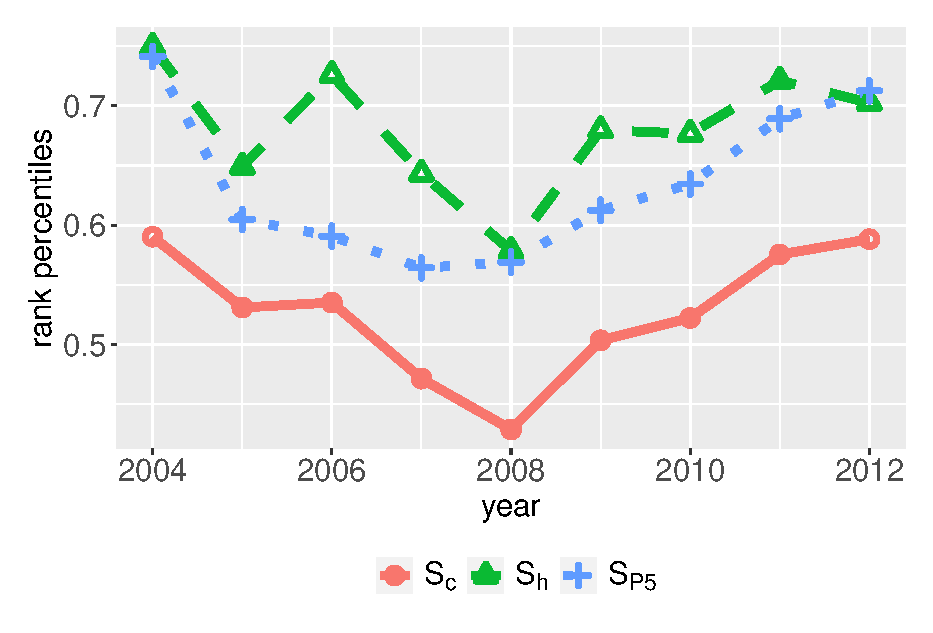
\includegraphics[width=0.6\textwidth]{figures/compare_autrp/auti.eps}
    \caption[rank percentile indicators for a random scholar]{The rank percentile indicators for a random scholar. The benchmark contains all tenured professors in the top-10 universities, as ranked by the U.S. News.}
    \label{fig:auti}
\end{figure}

The indicator S$_{P5}$ improves some major drawbacks of S$_c$ and S$_h$. First, it removes the seniority effect of publications. The evaluation metric for S$_c^{ib}(t)$ represents the citations that scholar $i$ receives by age $t$, which is the sum of citations for the scholar's publications by $t$. Compared to newly published works, publications with longer histories are more likely to attract citations and therefore contribute more to formulating S$_c$. A similar argument can be made for S$_h$. However, S$_{P5}$ treats the publications equally and evaluates them based on their performances at the publications' age of five. Additionally, a scholar who publishes a considerable number of low-impact works or participates in only a small number of high-impact projects can have a high value of S$_c$, since the absolute number of citations can be unlimited and is significantly influenced by extreme values. However, the S$_{P5}$ and S$_h$ of these scholars are not necessarily large, since these indicators limit the contribution of a single publication to be, at most, $1$ by definition of rank percentile and h-index score. Furthermore, compared to S$_h$, S$_{P5}$ penalizes scholars who are not truly innovative but carefully massage their h-index scores by publishing a number of papers that attract barely sufficient amounts of citations to increase their h-index scores. As long as a paper is among the top $h$ papers, the actual number of citations is irrelevant for h-index and S$_h$, but it can still impact S$_{P5}$. Finally, S$_{P5}$ requires less data compared to S$_c$ and S$_h$, since it only relies on the 5-year citation history of each publication. Hence, S$_{P5}$ is better suited to large-scale analysis.

We demonstrate the advantages of S$_{P5}$ by examining some extreme cases. We created three synthetic academic careers. Scholar A publishes a substantial number of publications throughout his/her career (more than $90\%$ of his/her cohorts in the benchmark), while all of the publications have little impact. Scholars B and C only publish one paper each at the beginning of their careers; B's paper is astonishing, while C's paper is average. Both scholars have an h-index equal to $1$ throughout their careers. Figure \ref{fig:simulated_authors} illustrates the rank percentile indicators for these three artificial scholars. We see that flooding low-impact publications can increase S$_c$ at the beginning of Scholar A's career. We also see that a single high-impact work improves the value S$_c$ throughout Scholar B's career; the author remains in the top $50\%$ at age $12$, as indicated by S$_c$. Both S$_{P5}$ and S$_h$ better characterize the performances of these authors. Finally, S$_h$ remains the same for Scholars B and C since they each have an h-index of $1$ throughout their careers. However, S$_{P5}$ considers that Scholar B's publication has a greater impact and therefore ranks higher than Scholar C. 

% fig:simulated_authors
% show the difference between various author rp
\begin{figure}[ht!]
    \centering
    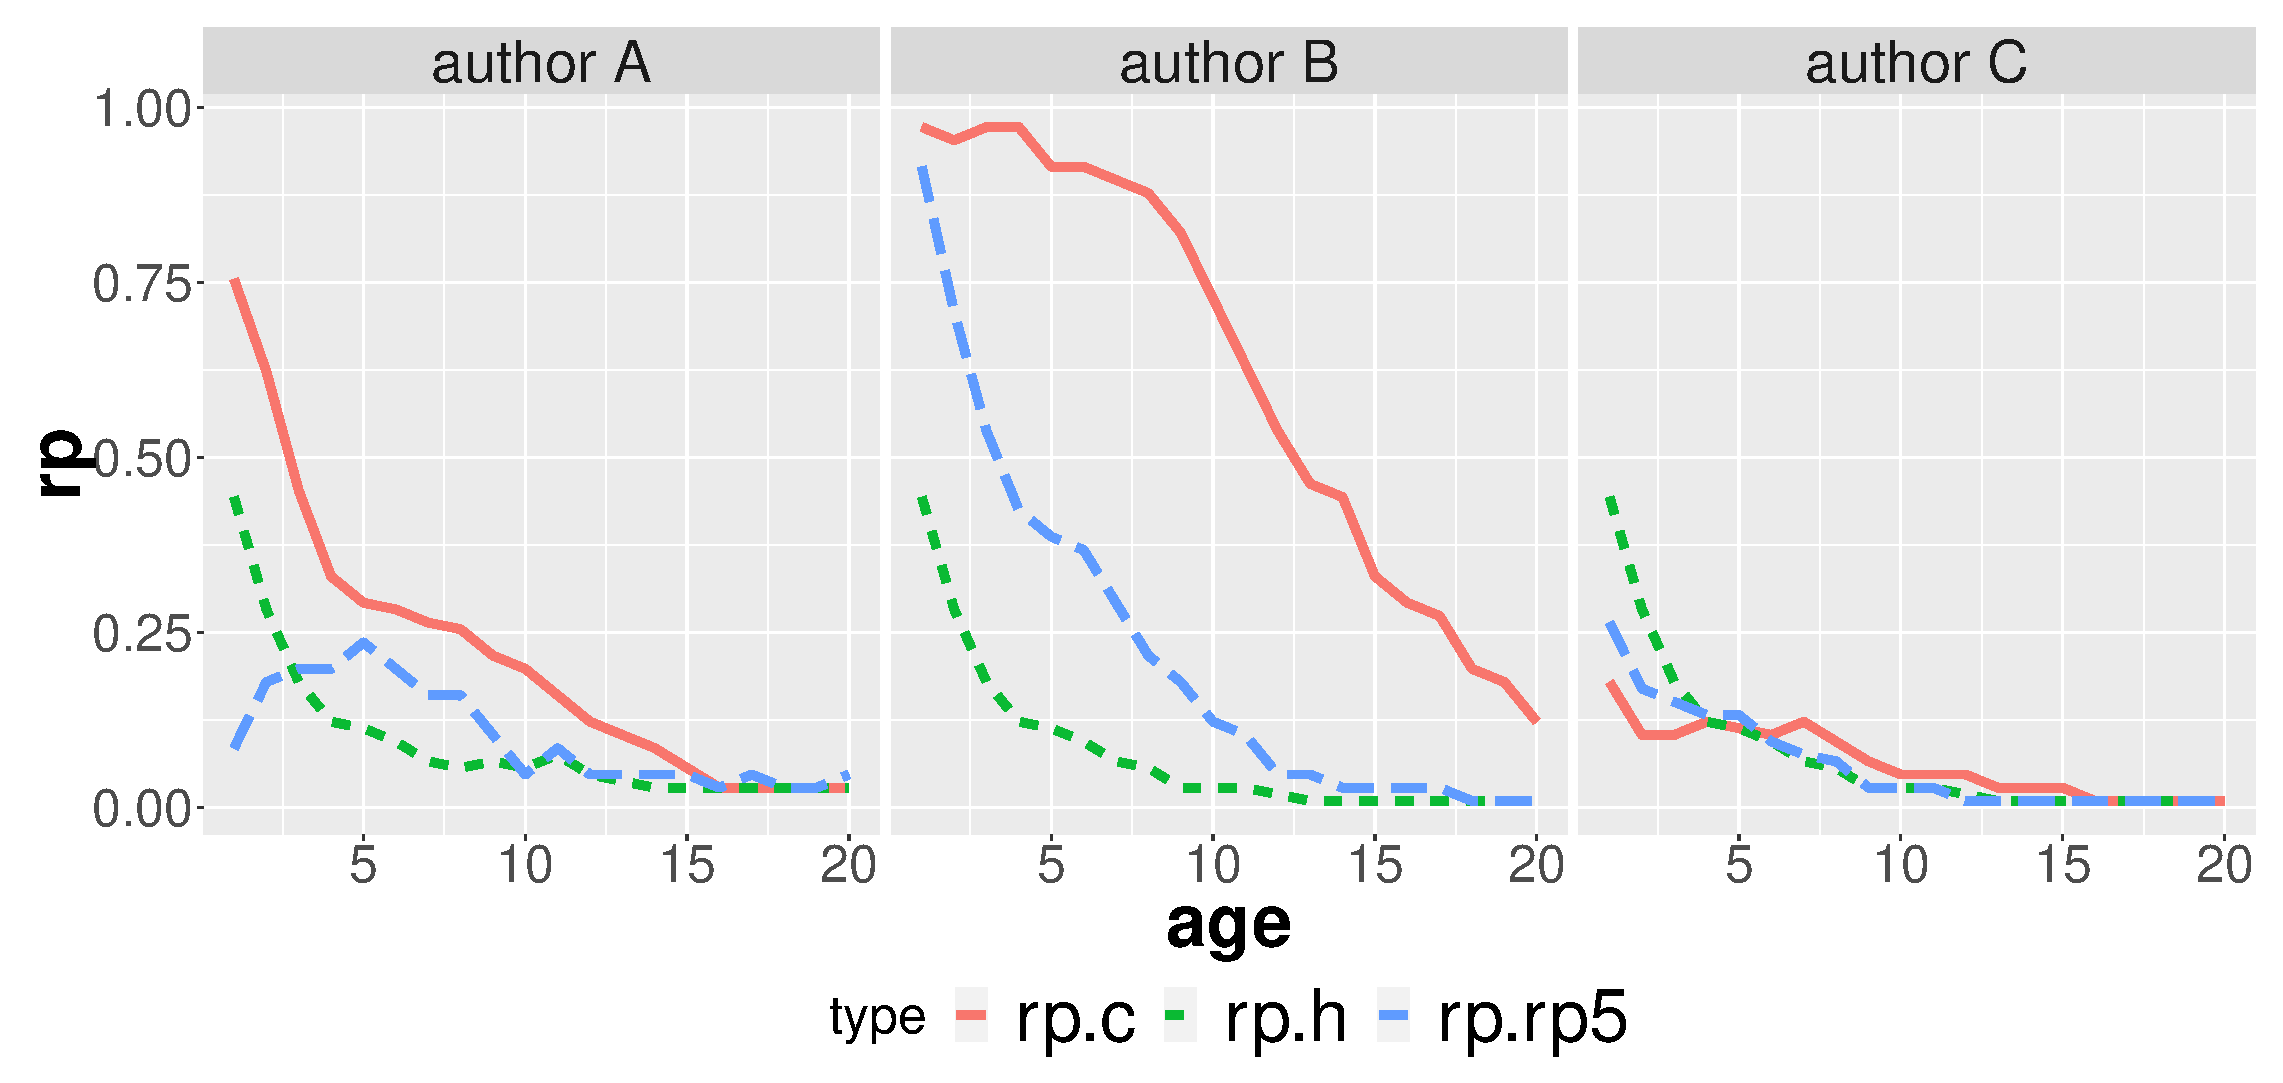
\includegraphics[width=\textwidth]{figures/compare_autrp/simulated_authors.eps}
    \caption[The advantage of S$_{it}^{P5}$ compared to other indicators]{Three artificial scholars illustrate the difference between various types of rank percentile indicators for scholars. Scholar A is highly productive at all ages, but all of the works have little impact. Scholars B and C only publish one paper each at age $1$; the paper of Scholar B has substantial impact, while the paper of Scholar C has medium impact. The h-index scores of Scholars B and C remain at $1$ throughout their careers. The benchmark includes scholars in biology who started their careers in $1990$.}
    \label{fig:simulated_authors}
\end{figure}

With the exception of the above-mentioned discrepancies, we present in Supplemental Material Section \ref{sec:suppl_similarity_autrp} that for the majority of scholars in our dataset, S$_{P5}$ largely agrees with S$_c$ and S$_h$. Furthermore, we consider utilizing various metrics to evaluate the publication, for example P$_c^{jb}(10)$ which is based on 10-year citation history. As we reveal Supplemental Material Section \ref{sec:suppl_robustness_P5}, the differences between the resultant rank percentile indicators and S$_{P5}$ are not statistically significant, thus indicating the robustness of S$_{P5}$. Intuitively, the publication percentile P$_c^{jb}(t)$ is highly stable over $t$, and therefore P$_c^{jb}(5)$ can be a reasonable indicator of the performance for the publication. The details will be discussed in the next section.

\section*{The predictability of rank percentile indicator}

In this section, we study the predictability of the rank percentile indicator. In general, we find the indicator to exhibit stability over time, and the indicator can be predicted via some simple linear regression models. 

\subsection*{The stationarity of the rank percentile indicator for scholars}

In the example of the tenure promotion, we utilized the rank percentile to compare the candidate with senior cohorts. The comparison is not valid if the candidate is more likely to attract citations than senior colleagues who started their careers years earlier. In such a case, it may well be the academic environment that results in a better performance of the candidate rather than the internal factors, such as creativity and productivity.

Figure \ref{fig:rp_stationarity} portrays S$_{P5}$ at age $10$, grouped by the starting year of academic careers. We see that S$_{P5}$ does not exhibit an obvious trend and is approximately stationary over the starting year of careers, thus providing empirical evidence for the validity of the rank percentile. 

\begin{figure}[ht!]
    \centering
    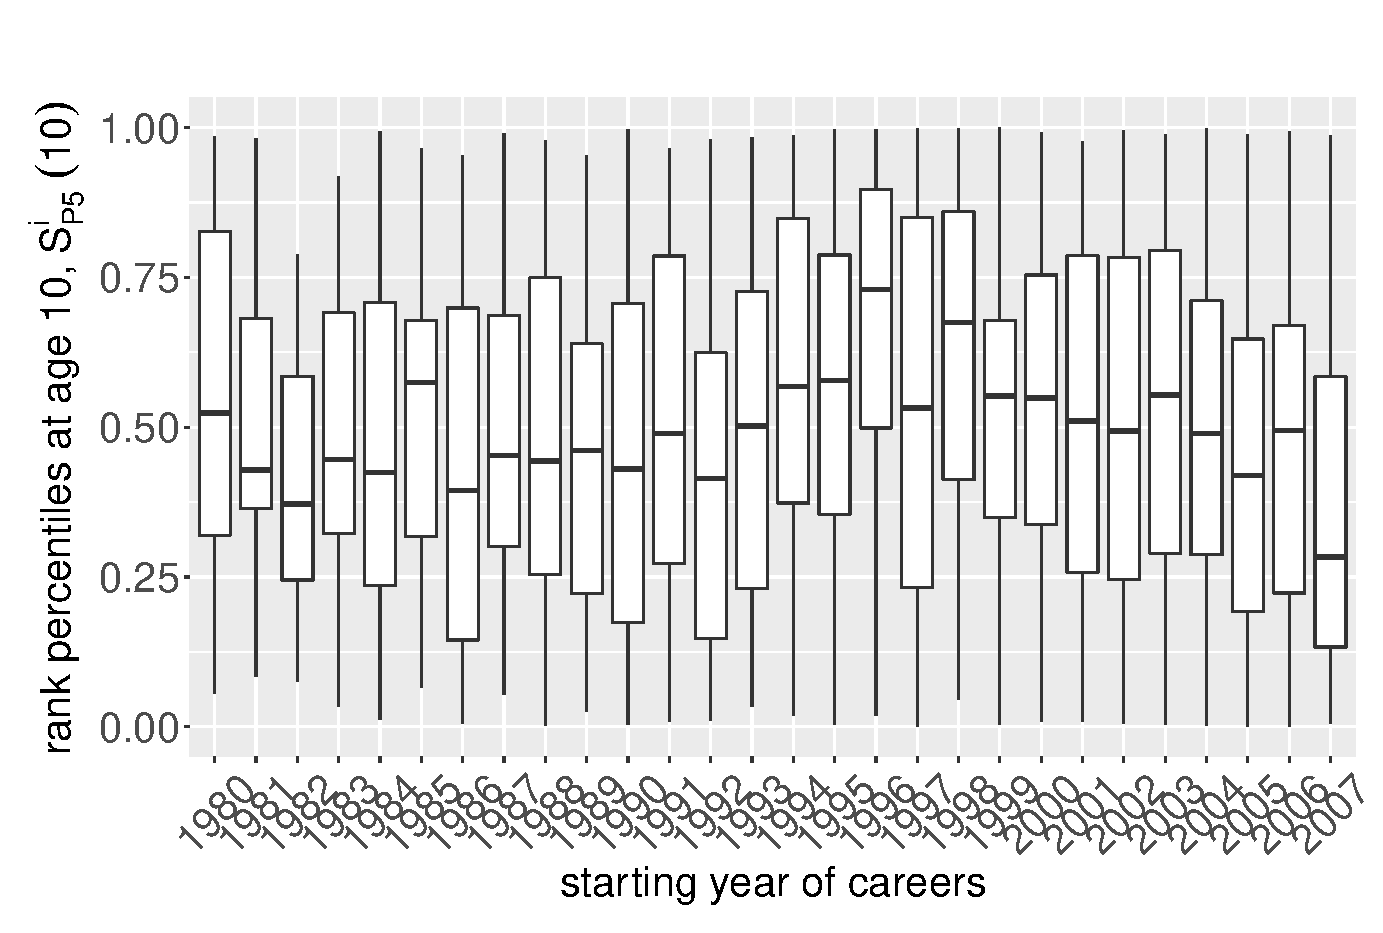
\includegraphics[width=0.6\textwidth]{figures/stationarity/rp_stationarity.eps}
    \caption[Stationarity of rank percentile indicators]{S$_{P5}(10)$ grouped by the starting years of academic careers. The benchmark contains all tenured professors in the top-10 universities, as ranked by the U.S. News.} 
    \label{fig:rp_stationarity}
\end{figure}

\subsection*{The predictability of rank percentile indicator}

Citations have been proven to lack long-term predictive power~\cite{Wang2013}. Figure \ref{fig:pred_cit_age} illustrates that papers with the same citations by the fifth year since published can have noticeably different citation paths and long-term effects. Additionally, exceptional and creative ideas typically require a lengthy period to be appreciated by the scientific community. As presented in Figure \ref{fig:pred_cit_cit}, the correlation between short- and long-term citations breaks down for the most highly-cited publications (the shaded rectangle). These problems can be largely avoided by utilizing rank percentile indicators, as evidenced in Figures \ref{fig:pred_rp_age} and \ref{fig:pred_rp_rp}. The considerable variation in the long-term effect of citations is restricted by utilizing rank percentiles. For publications with high impact, the correlation between short- and long-term effects persists when utilizing rank percentiles.

% publication rank percentile vs citations, predictability, Wang(2013)
\begin{figure}[ht!]
    \centering
    \begin{subfigure}[b]{0.48\textwidth}
     \centering
     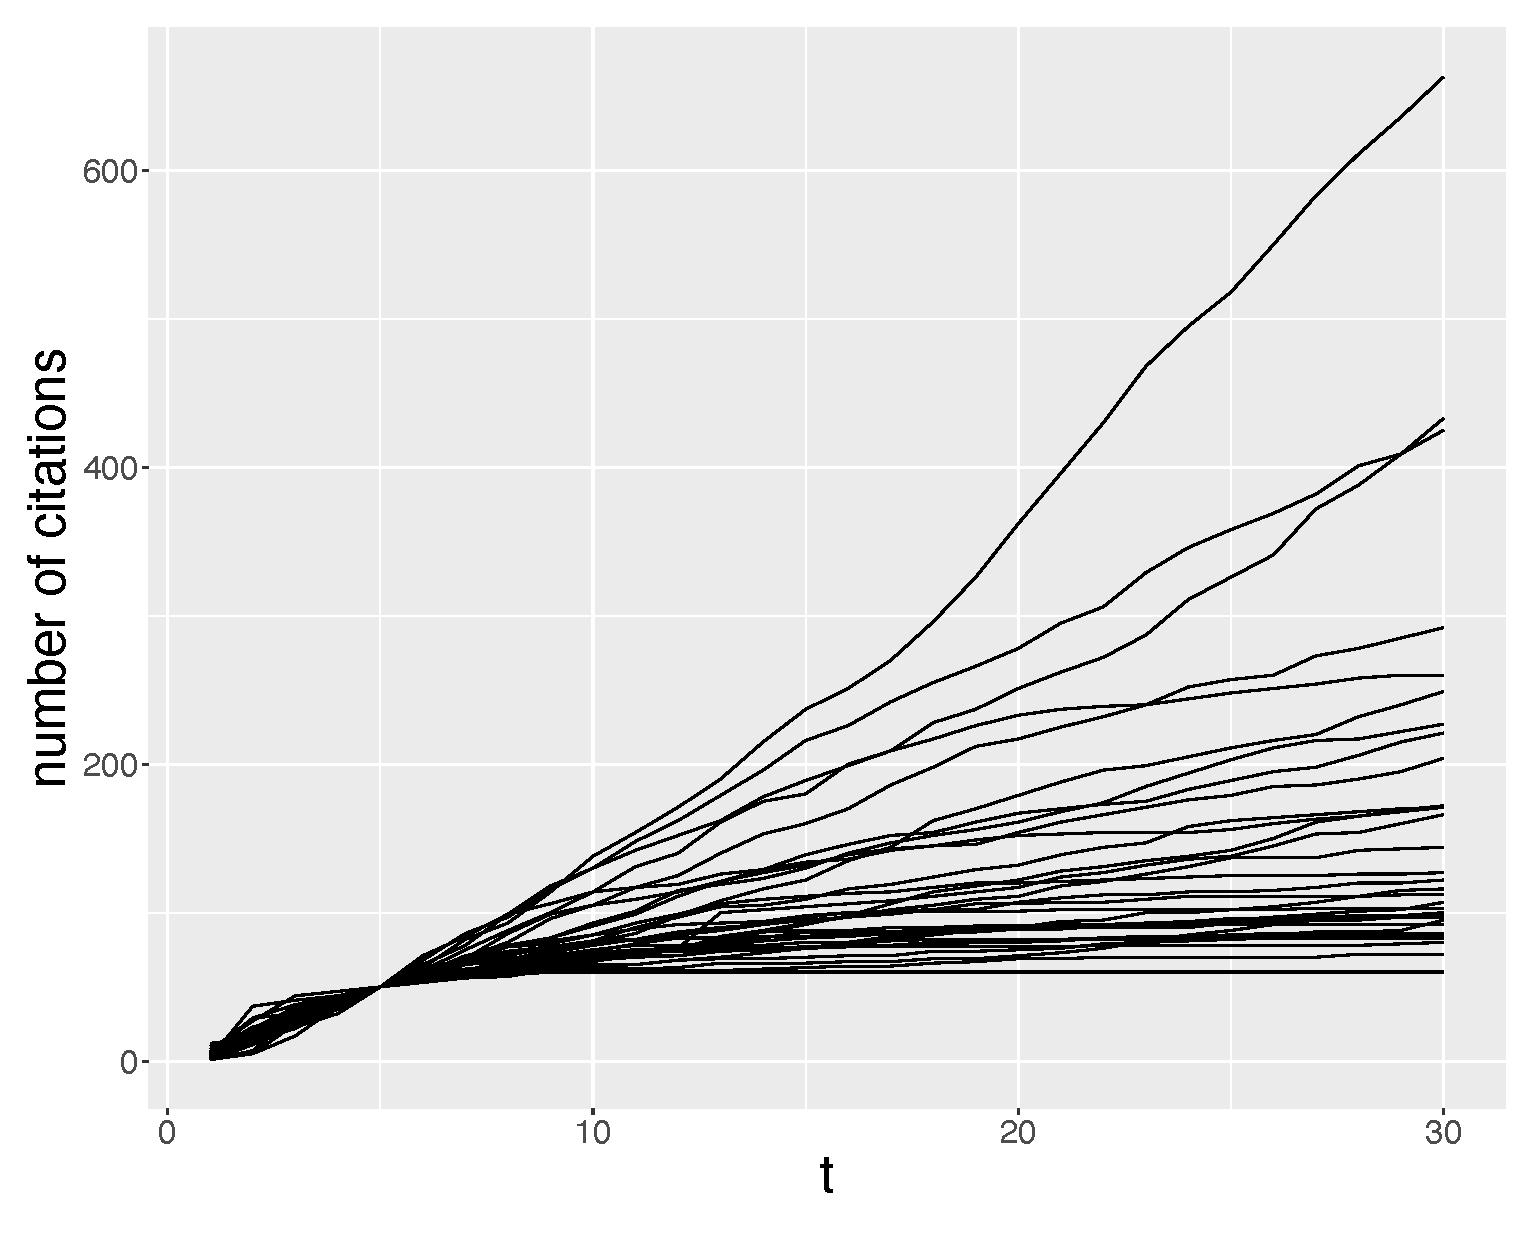
\includegraphics[width=\textwidth]{figures/pred_power/cit_t.eps}
     \caption{Number of citations versus age}
     \label{fig:pred_cit_age}
    \end{subfigure}
    \hfill
    \begin{subfigure}[b]{0.48\textwidth}
     \centering
     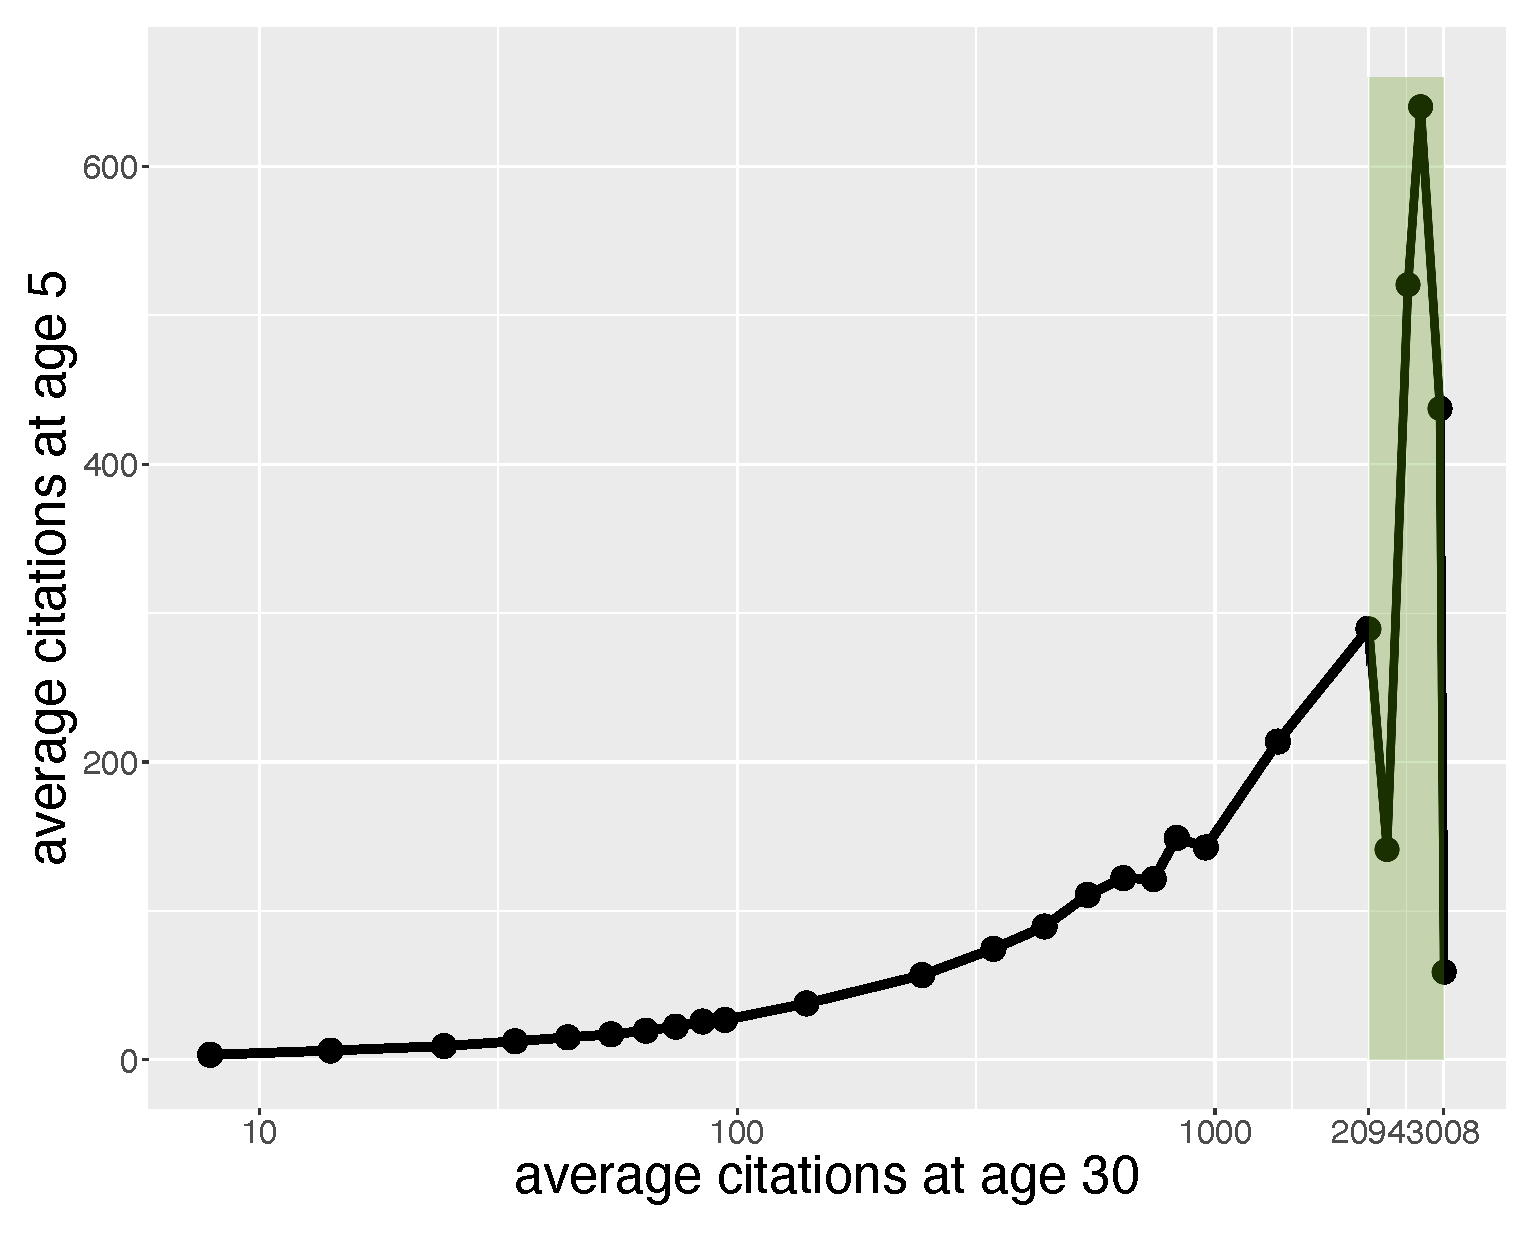
\includegraphics[width=\textwidth]{figures/pred_power/cit_cit.eps}
     \caption{Average citations at age $5$ versus those at age $30$}
     \label{fig:pred_cit_cit}
    \end{subfigure}
    \caption[Predictability of citations]{The predictability of citations. The benchmark contains the publications in biology. Figure \ref{fig:pred_cit_age} portrays the cumulative citations for publications that have $50$ citations by the fifth year since published. Figure \ref{fig:pred_cit_cit} displays the average citations by age $5$ versus the average citations by age $30$. The averages are calculated over groups of publications, which are prespecified by dividing the range of citations by age $30$ into equal intervals on the log scale. Note that we do not claim the originality of the figures, which have been illustrated via a different dataset~\cite{Wang2013}.}
    \label{fig:pub_cit_pred}
\end{figure}


\begin{figure}[ht!]
    \centering
    \begin{subfigure}[b]{0.495\textwidth}
     \centering
     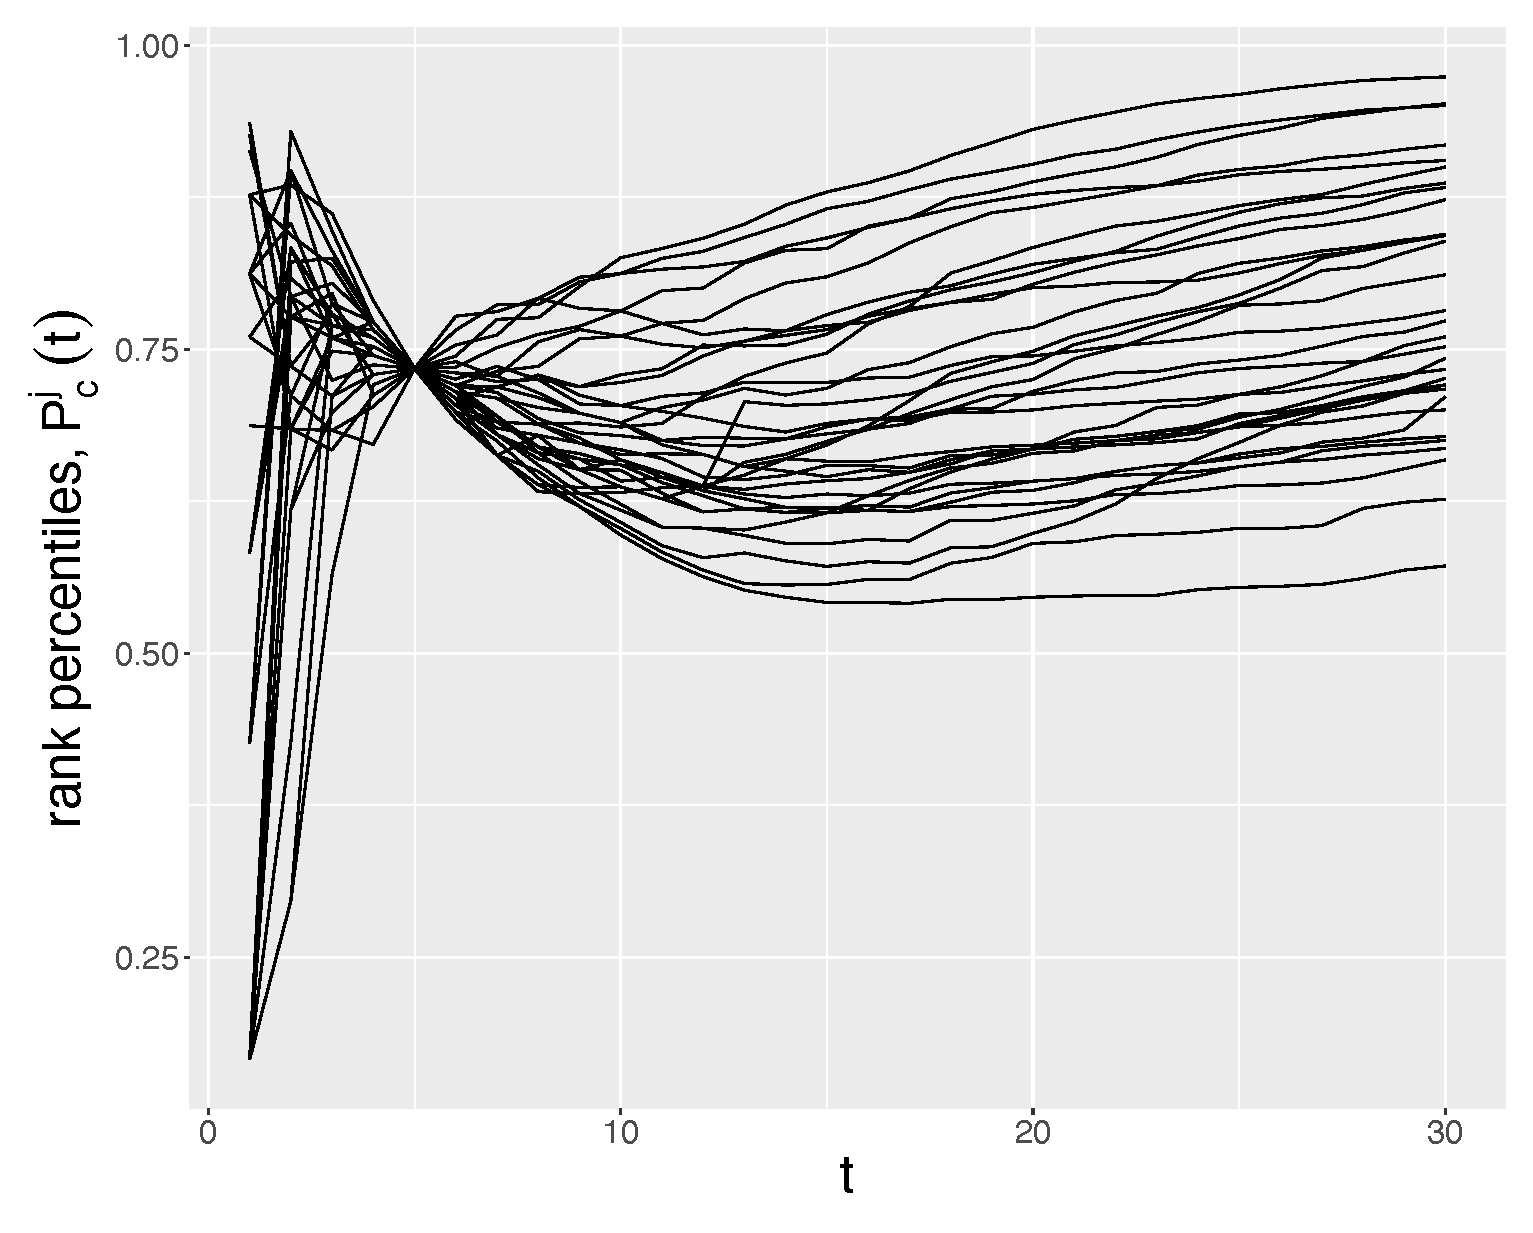
\includegraphics[width=\textwidth]{figures/pred_power/rp_t.eps}
     \caption{Rank percentiles P$_c$ versus age}
     \label{fig:pred_rp_age}
    \end{subfigure}
    \hfill
    \begin{subfigure}[b]{0.495\textwidth}
     \centering
     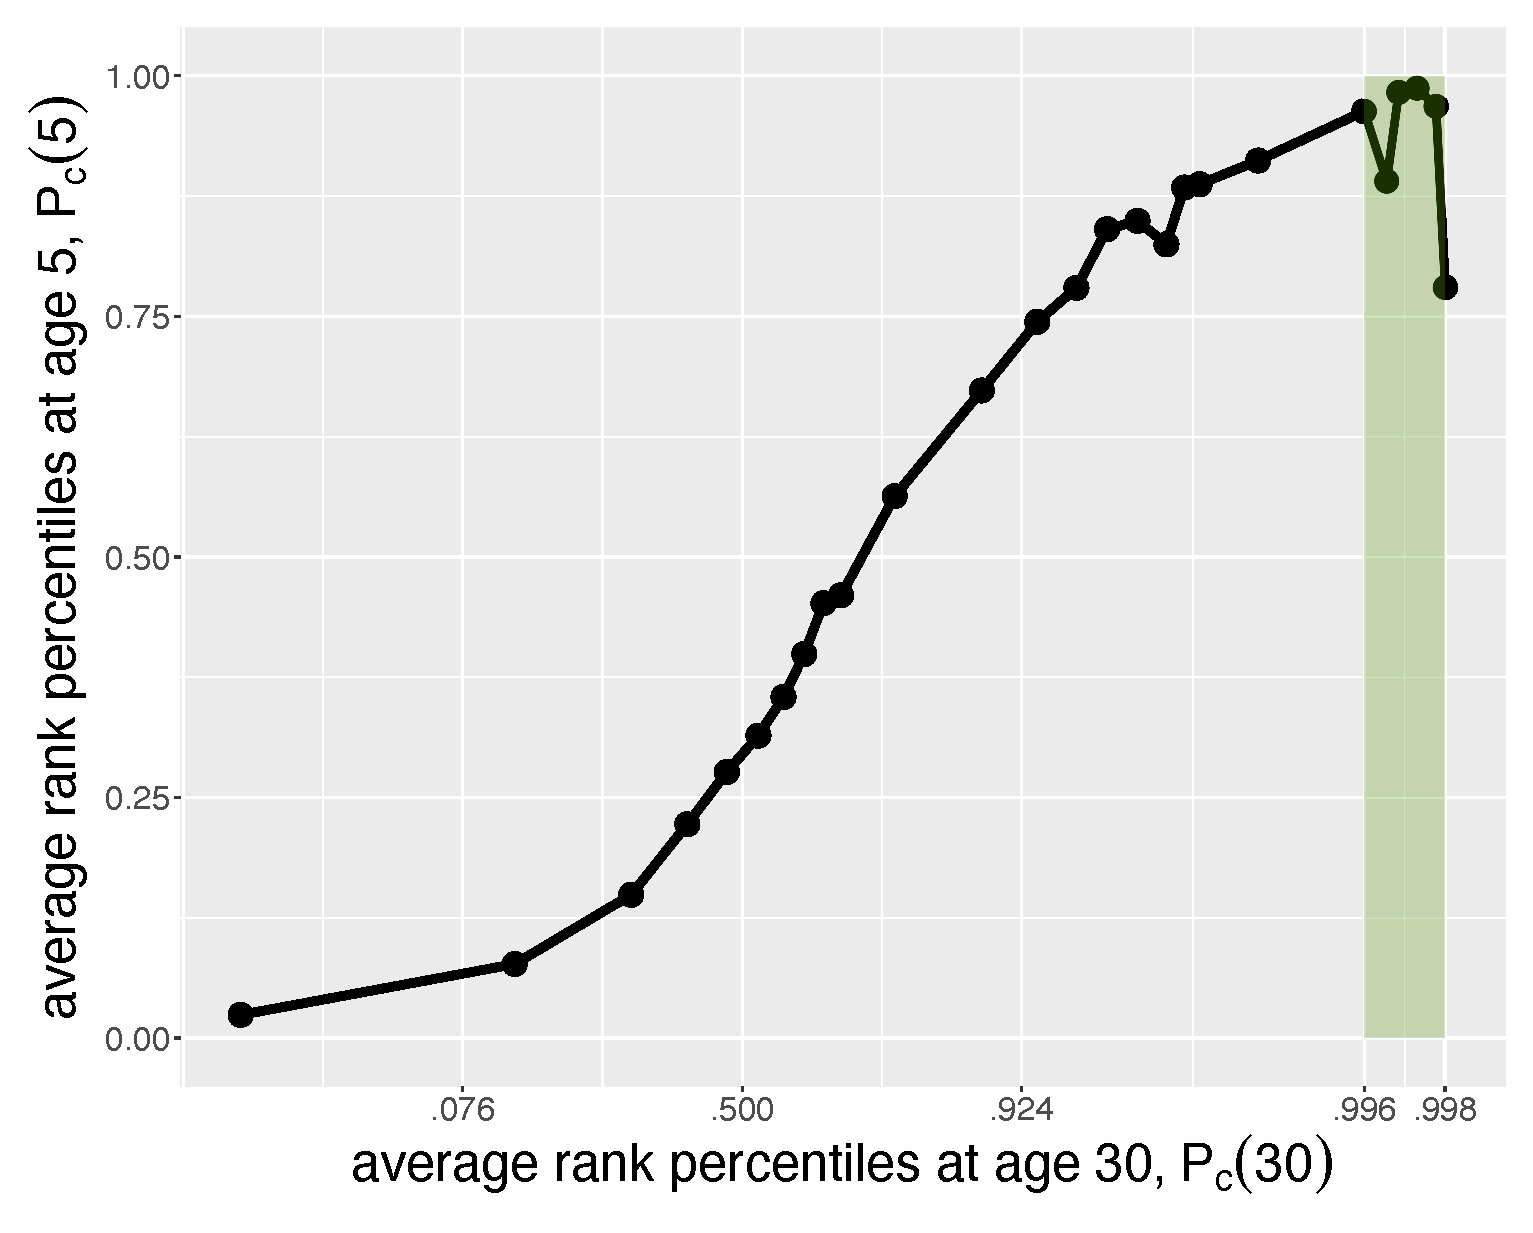
\includegraphics[width=\textwidth]{figures/pred_power/rp_rp.eps}
     \caption{Average P$_c$ at age $5$ versus those at age $30$}
     \label{fig:pred_rp_rp}
    \end{subfigure}
    \caption[Predictability of rank percentiles]{The predictability of rank percentiles. Figure \ref{fig:pred_rp_age} demonstrates the rank percentiles for the publications considered in Figure \ref{fig:pred_cit_age}. Figure \ref{fig:pred_rp_rp} presents the average of P$_c(5)$ versus the average of P$_c(30)$ for the same groups of publications as in Figure \ref{fig:pred_cit_cit}.}
    \label{fig:pub_rp_pred}
\end{figure}

We further characterize the predictability of rank percentile indicators. Figure \ref{fig:hm_rp_pub} presents the correlation between rank percentiles at two ages, P$_c^{jb}(t_1)$ and P$_c^{jb}(t_2)$ where $t_1<t_2$. We noticed overall large correlations for both benchmarks. The correlation diminishes as the forecast horizon $(t_2-t_1)$ increases, which simply reflects the difficulty of long-term forecasting. Additionally, the correlation increases as $t_1$ increases while holding the forecast horizon fix. This indicates that the performance of a senior publication is easier to predict, since the longer history removes more uncertainties regarding its performance. We further noticed a slightly higher predictive power when we restricted the benchmark to be the area of biology. 

Figure \ref{fig:hm_rp_aut} illustrates that the patterns discussed above generally hold for rank percentiles of scholars. The magnitude of correlations is smaller than those for publications, especially for long-term forecasts. This results from the fact that forecasting the future impact of future works is considerably more difficult than forecasting the future impact of existing works. Intuitively, predicting S$_{P5}^{ib}(t_2)$ involves predicting the performance of papers published before $t_1$ and predicting the performance of those published between $t_1$ and $t_2$. The former is predicting the future impact of existing works, while the latter is predicting the future impact of future works. However, predicting the publication indicator P$_c^{jb}(t_2)$ only involves predicting the future impact of publication $j$, which is a considerably easier task. Furthermore, when the forecast horizon increases while fixing $t_1$, additional future works are involved in predicting S$_{P5}^{ib}(t_2)$; therefore, we see that the correlation decreases more quickly than when we predict P$_c^{jb}(t_2)$. 

% publication rank percentile, heat map of correlations
\begin{figure}[ht!]
    \centering
    \begin{subfigure}[b]{0.8\textwidth}
        \centering
             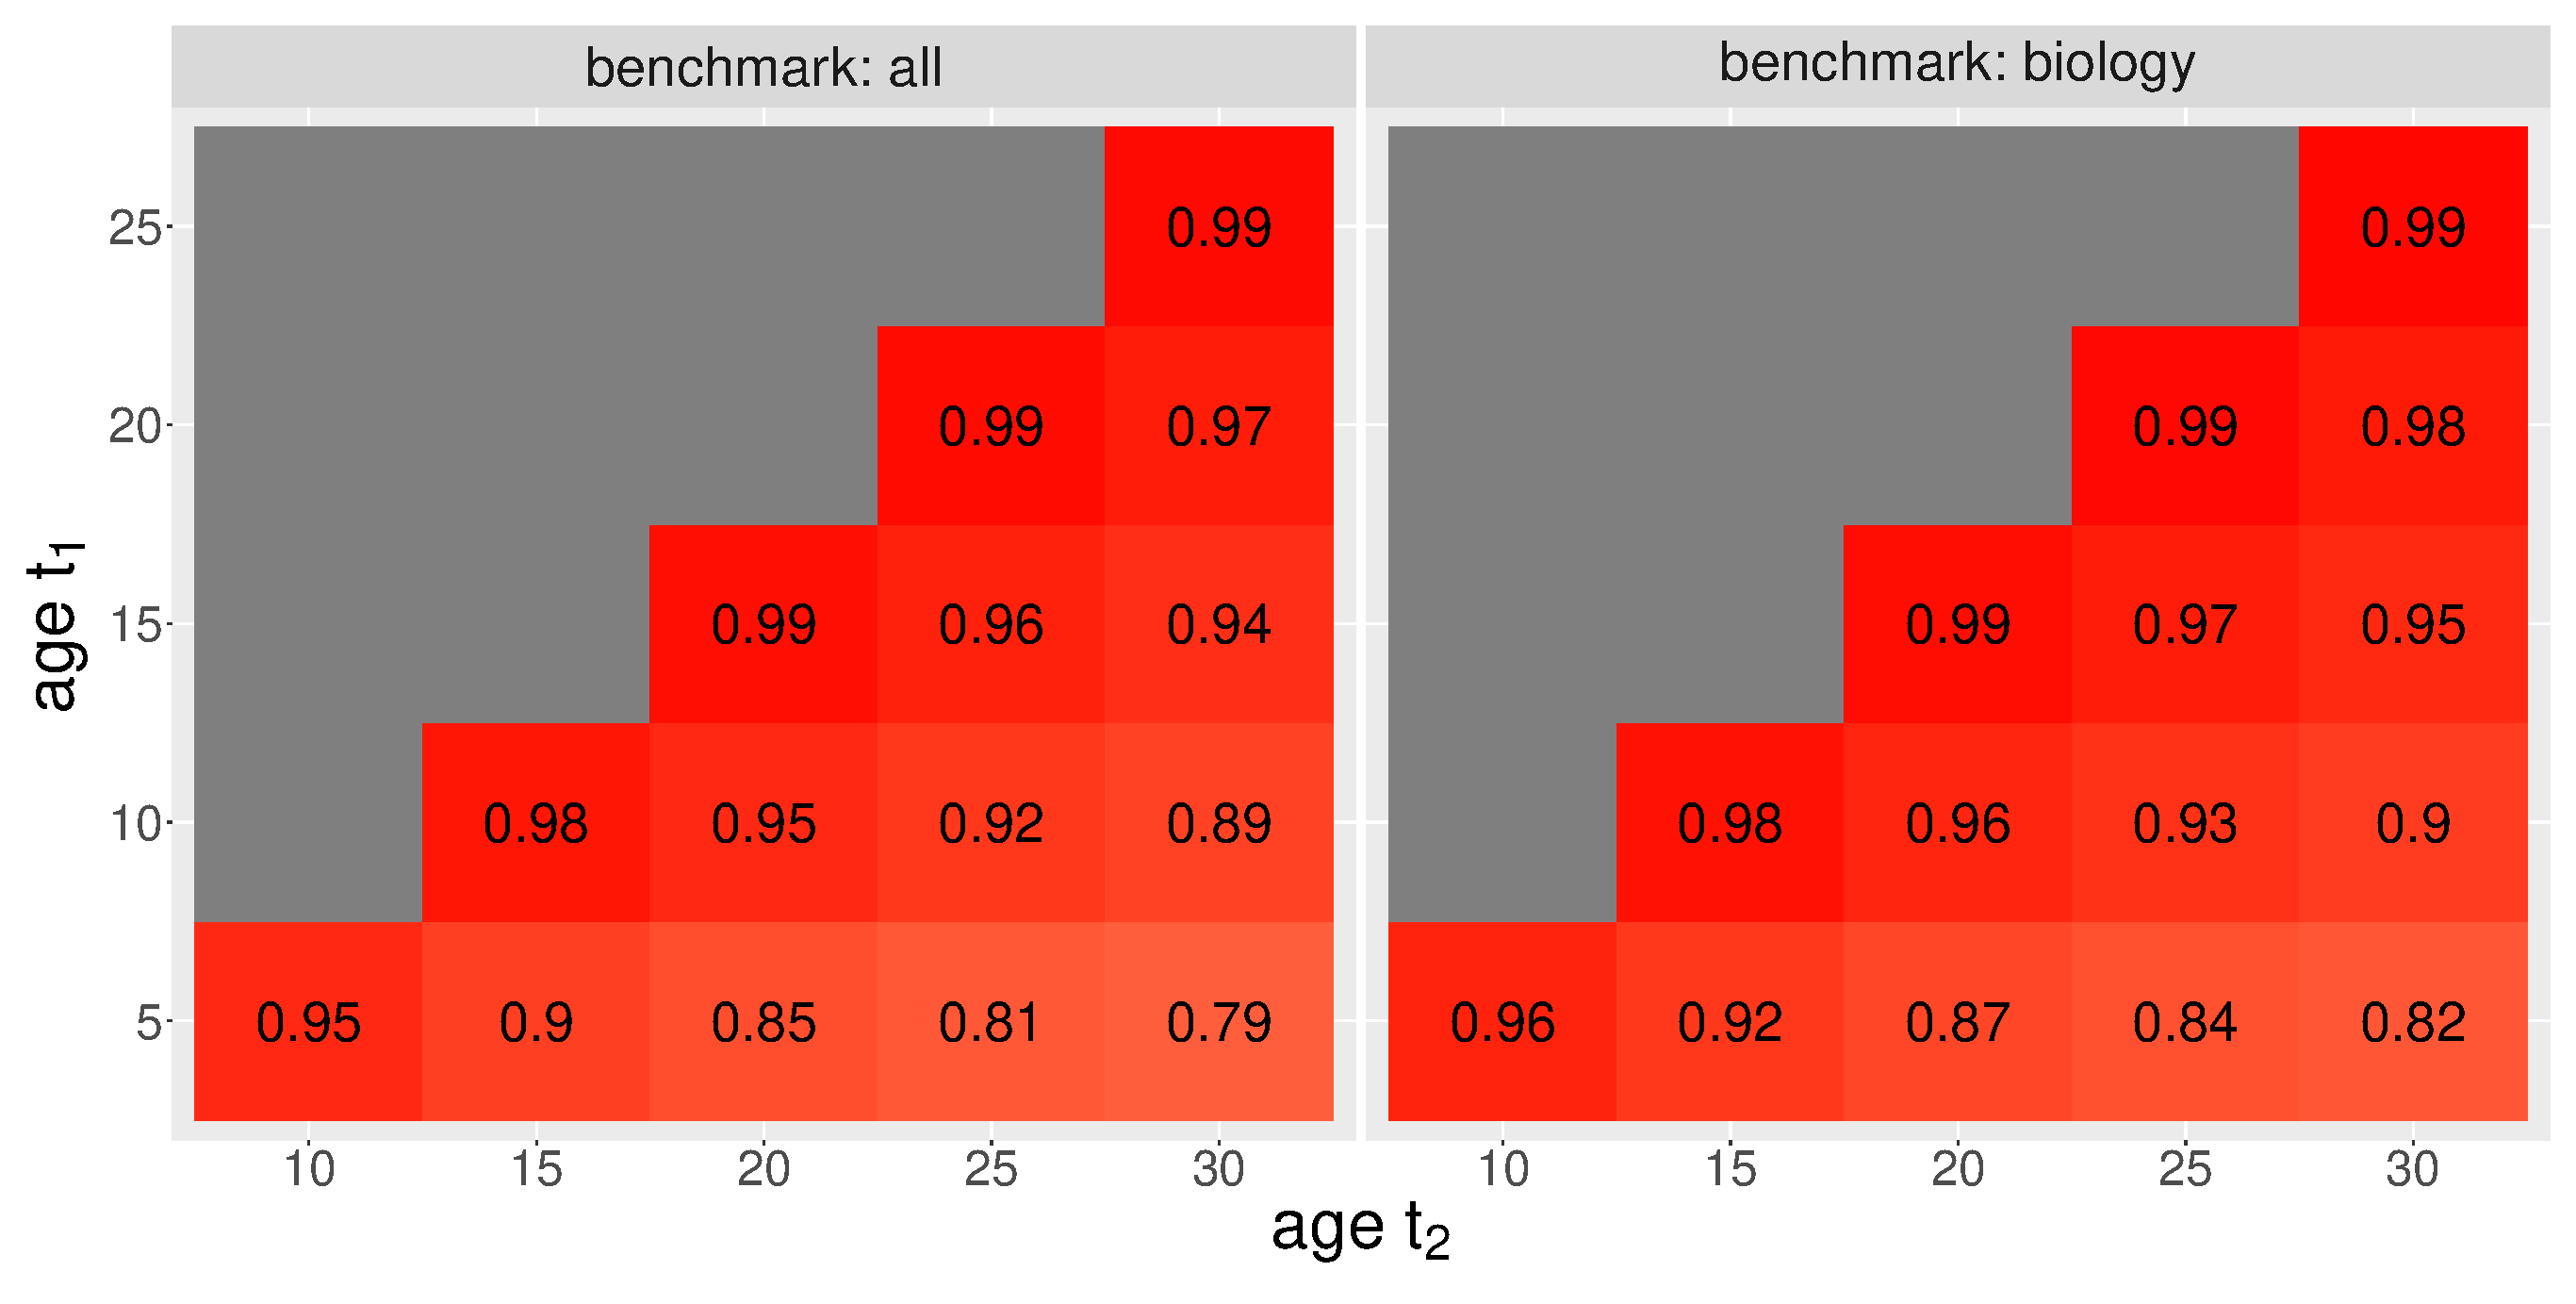
\includegraphics[width=\textwidth]{figures/pred_power/heatmap_cor_pub.eps}
         \caption{Correlation between P$_c^{jb}(t_1)$ and P$_c^{jb}(t_2)$}
         \label{fig:hm_rp_pub}
    \end{subfigure}

    \begin{subfigure}[b]{0.8\textwidth}
        \centering
             \includegraphics[width=\textwidth]{figures/pred_power/heatmap_cor_aut.eps}
         \caption{Correlation between S$_{P5}^{ib}(t_1)$ and S$_{P5}^{ib}(t_2)$}
         \label{fig:hm_rp_aut}
    \end{subfigure}

    \begin{subfigure}[b]{0.8\textwidth}
        \centering
             \includegraphics[width=\textwidth]{figures/pred_power/heatmap_cor_aut_future.eps}
         \caption{Correlation between S$_{P5}^{ib}(t_1)$ and S$_{P5}^{ib}(t_2 | t_1)$}
         \label{fig:hm_rp_aut_future}
    \end{subfigure}
    \caption[Correlations between rank percentiles at different ages]{The Pearson's correlation between rank percentile indicators at two different ages. }
    \label{fig:hm_rp}
\end{figure}

\begin{figure}[ht!]
    \centering
    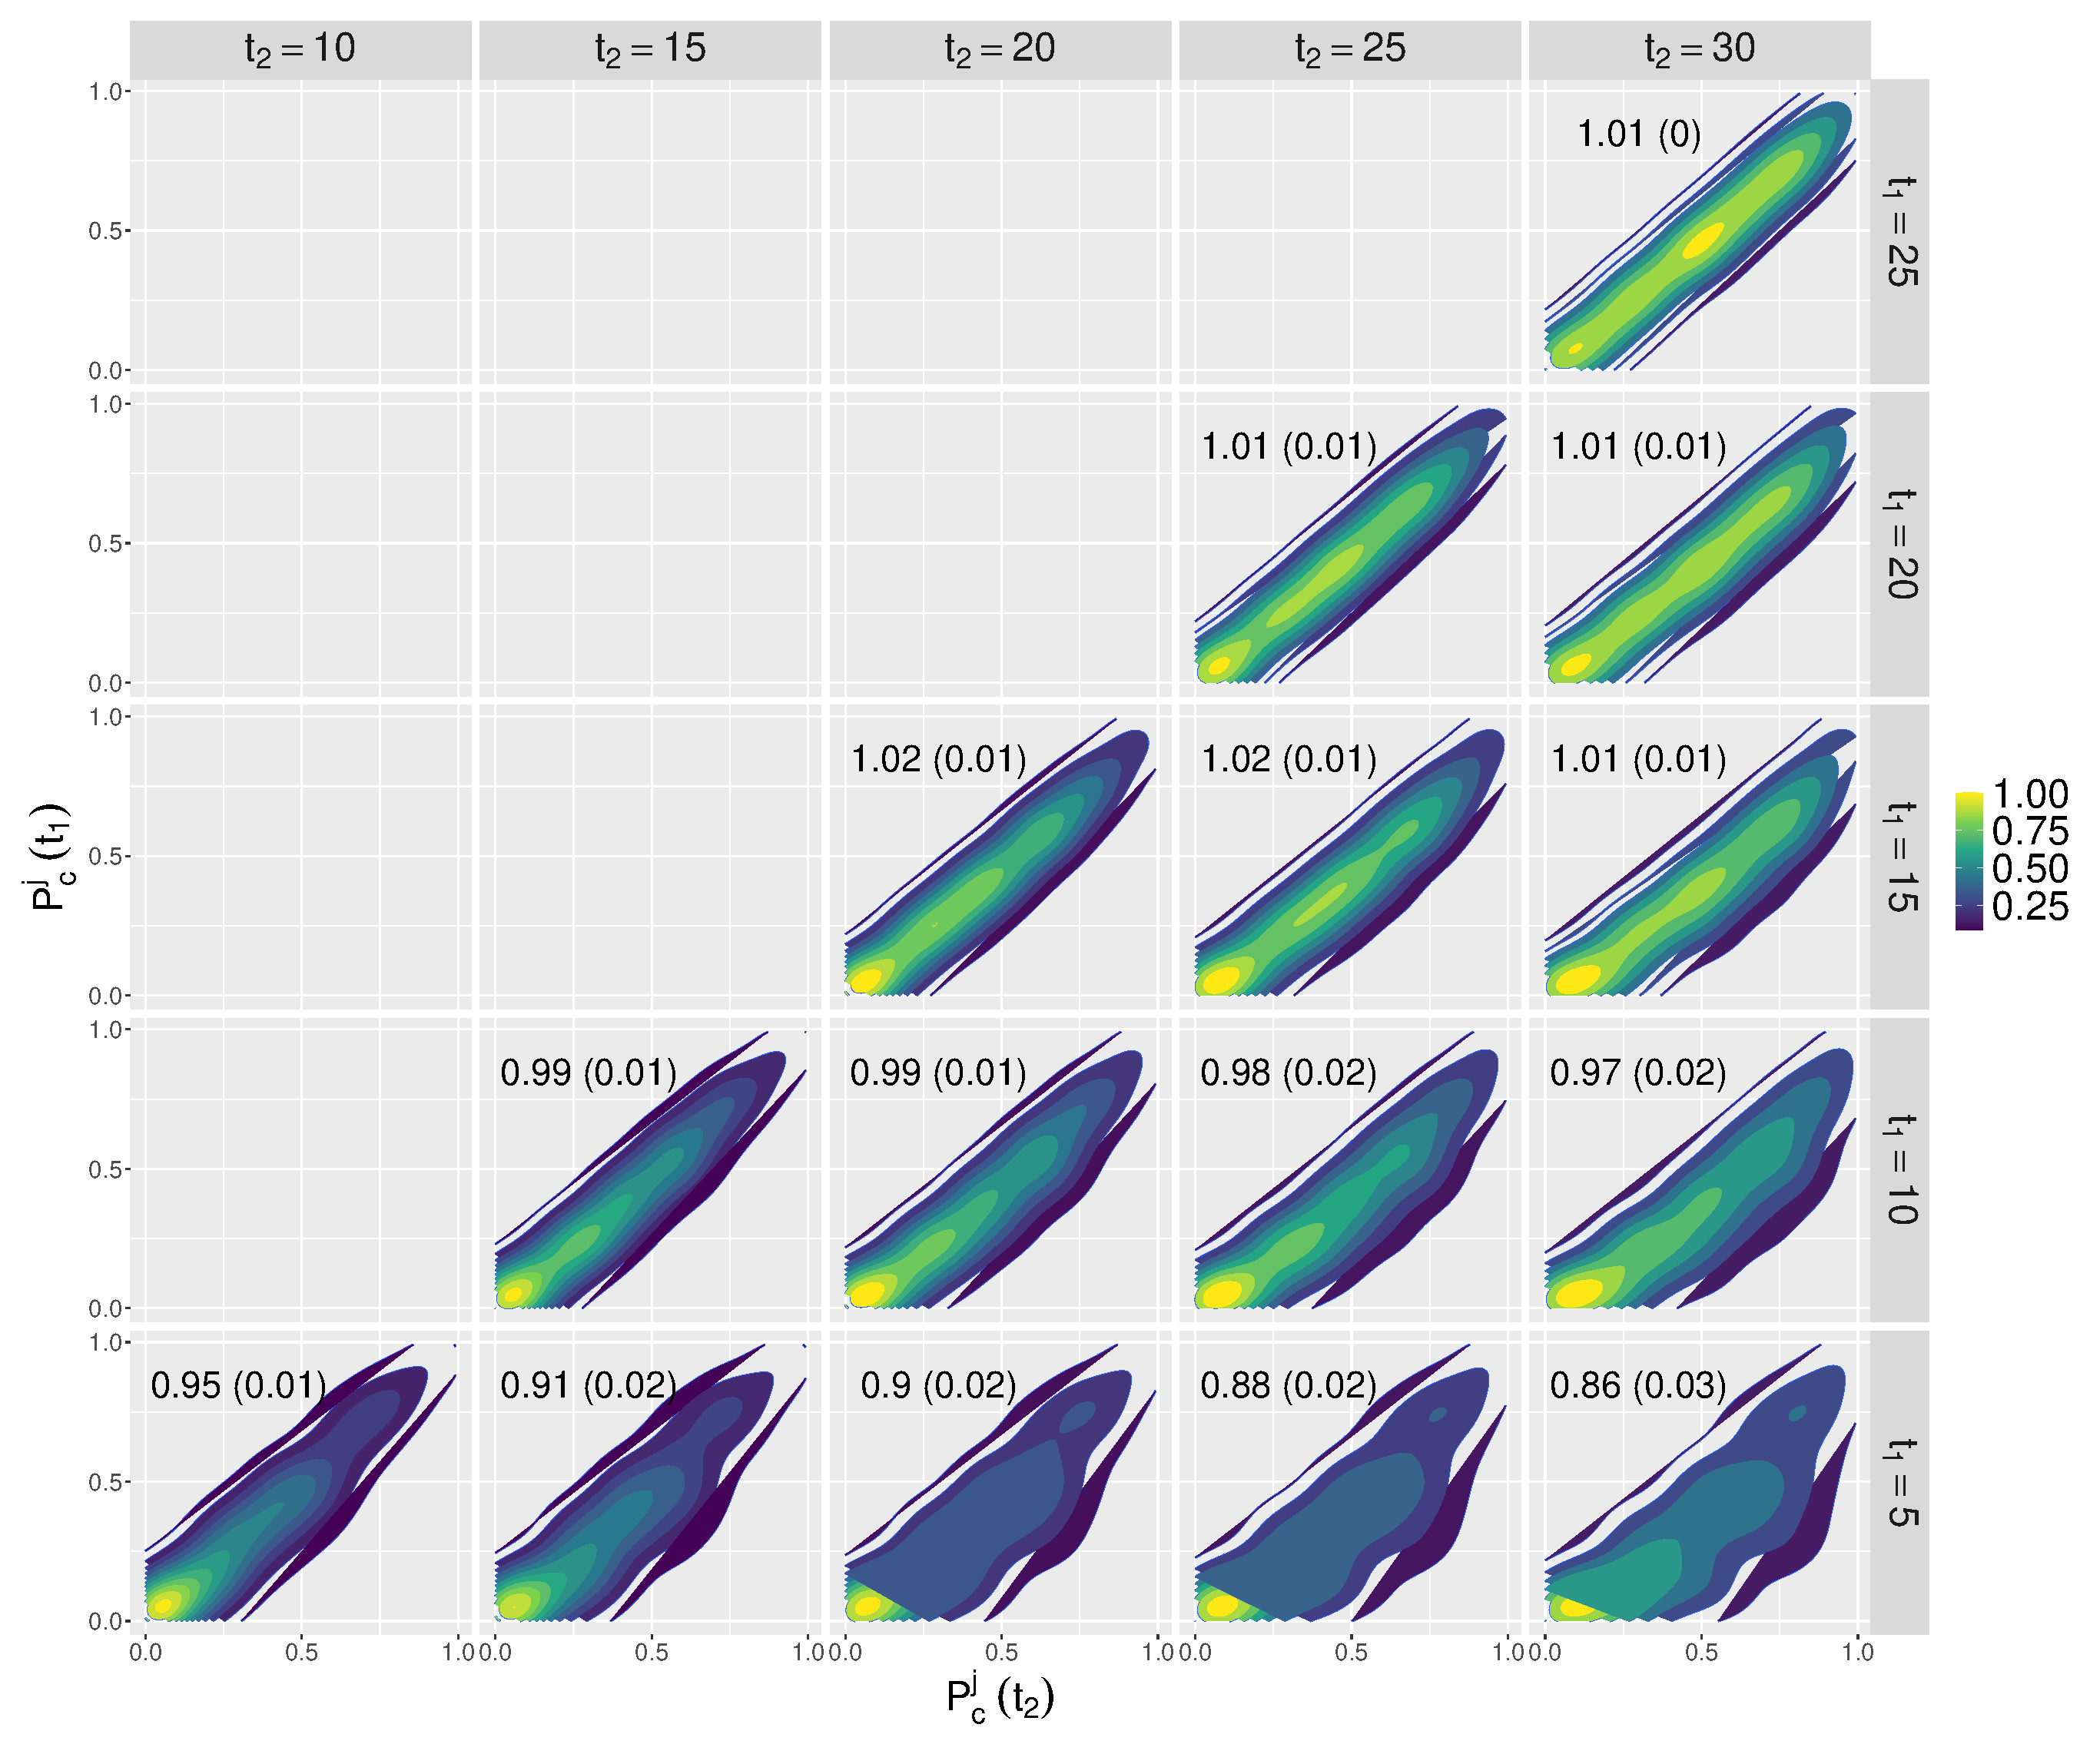
\includegraphics[width=\textwidth]{figures/pred_power/scatter_pubrp_bio1980.eps}
    \caption[Kernel density estimation for the scatter points of P$_c(t_1)$ and P$_c(t_2)$]{Kernel density estimation for the scatter points of P$_c^{jb}(t_1)$ and P$_c^{jb}(t_2)$. We also fitted a simple linear regression of P$_c^{jb}(t_2)$ on P$_c^{jb}(t_1)$. The estimated coefficient and the corresponding standard error (in parentheses) are displayed in each plot. The benchmark here includes publications in biology that were published in $1980$.}
    \label{fig:scatter_pubrp_bio1980}
\end{figure}


The strong linear relationship between P$_{c}^{jb}(t_1)$ and P$_c^{jb}(t_2)$ is further characterized in Figure \ref{fig:scatter_pubrp_bio1980}. The data are along the $45 \degree$ line, and the linear regression coefficient of P$_c^{jb}(t_2)$ on P$_c^{jb}(t_1)$ is close to $1$ with small standard errors, thus indicating the high stability of P$_c$. A similar figure for S$_{P5}$ is displayed in Supplemental Material Figure \ref{fig:scatter_autrp_all}, in which we find that S$_{P5}$ exhibits short-term stability.

Predicting S$_{P5}^{ib}(t_2)$ can assist in decision making for faculty positions or granting tenure, since the committee would like to examine the cumulative scientific impact of the scholar. In assigning research funding or allocating research resources regarding planned studies and potential future publications, the future impact of future works is often of interest. We utilize S$_{P5}^{ib}(t_2|t_1)$ to denote the rank percentile indicator calculated based on papers published between $t_1$ and $t_2$. Figure \ref{fig:hm_rp_aut_future} illustrates the correlation between S$_{P5}^{ib}(t_1)$ and S$_{P5}^{ib}(t_2|t_1)$. The magnitudes of correlation are moderately high, indicating an approximately linear relationship, although the strength is not as strong as it was in predicting the cumulative impact, that is, predicting S$_{P5}^{ib}(t_2)$, which is consistent with our expectation.

\subsection*{Predictive models}
We now formulate the prediction tasks as supervised learning problems, and we illustrate that the rank percentile indicators can be predicted via simple linear models. We consider the following fitting procedures; these models are ordered by increasing complexity:
\begin{itemize}
    \item Baseline: simple linear regression model.
    \item Simple Markov model (sm).
    \item Penalized linear regression models, including the ridge~\cite{hoerl1970ridge}, lasso~\cite{Tibshirani1996}, elastic net (enet)~\cite{zou2005regularization} and the Gamma lasso (gamlr)~\cite{Taddy2017}.
    \item Ensemble methods of regression trees, including the random forest (rf)~\cite{liaw2002classification} and extreme gradient boosting trees (xgbtree)~\cite{chen2016xgboost}.
    \item Neural networks (nnet).
\end{itemize}

The baseline model fits a simple linear regression of the target variable on the autoregressive feature, e.g. P$_c^{jb}(t_1)$ for predicting the publication impact. The simple Markov model further considers the change of the autoregressive feature in the past two ages, e.g. P$_c^{jb}(t_1)$-P$_c^{jb}(t_1-2)$, in addition to the autoregressive feature and fits a linear regression model. 

\subsubsection*{Features and model fitting}

For the rest of the methods, we created an extensive list of features based on the citation histories. The features are characterized as either scholar- or publication-based features. For example, to predict the scholar indicator S$_{P5}^{ib}(t_2)$, a scholar-based feature is the number of papers that scholar $i$ publishes by age $t_1$, and a publication-based feature is the average number of citations for these papers. We established a total of $30$ features for predicting the publication indicator and $42$ features for predicting the scholar indicator, which can be found in the Supplemental Material Tables \ref{tab:features_pubrp} and \ref{tab:features_autrp}, respectively. Note that many of the features have been utilized when formulating the prediction task for number of citations and h-index scores~\cite{acuna2012future,weihs2017learning}.

The features were created utilizing the citation information available by $t_1$, and the dependent variable was specified at $t_2$. The data was split into the training and testing set based on a 9:1 ratio. We considered five stages of a publication or a scholar, that is, $t_1\in\{5,10,15,20,25\}$, and we forecasted up to $30$ years of age, that is, $t_2=t_1+1,\cdots,30$; this resulted in $75$ pairs of $(t_1,t_2)$ in total. The models were independently trained $75$ times. 

We also noted (in the Supplemental Material Section \ref{sec:suppl_stationarity}) that both S$_{P5}$ and P$_c$ are non-stationary time series, as evidenced by the Dicky-Fuller test~\cite{dickey1979distribution} and the KPSS test~\cite{kwiatkowski1992testing}. The differenced series are stationary (also presented in the Supplemental Material) and are utilized as the response variable, that is $\Delta \text{P}_{c}^{jb}(t_2) = \text{P}_{c}^{jb}(t_2) - \text{P}_{c}^{jb}(t_1)$, $\Delta \text{S}_{P5}^{ib}(t_2) = \text{S}_{P5}^{ib}(t_2) - \text{S}_{P5}^{ib}(t_1)$, and $\Delta \text{S}_{P5}^{ib}(t_2|t_1) = \text{S}_{P5}^{ib}(t_2|t_1) - \text{S}_{P5}^{ib}(t_1)$. Note that the stationarity discussed here characterizes the property of S$_{P5}$ and P$_c$ as time series. It is different from the stationarity as discussed in Figure \ref{fig:rp_stationarity}, where we fix $t=10$ and examine the stationarity of S$_{P5}(10)$ over the starting year of the scholars' careers.

The machine learning methods were trained using \textit{R}~\cite{RCT2019} with the package \textit{mlr}~\cite{Bischl2016}, which provides a pipeline of training, validating, and testing for the model. The lasso, ridge, elastic net, random forest, and xgbtree are inbuilt learners of the package. The Gamma lasso and neural network were trained utilizing \textit{R} packages \textit{gamlr}~\cite{Taddy2017} and \textit{keras}~\cite{Allaire2019}, respectively. 

The machine learning methods require hyperparameter tuning, which involves deciding the search space of parameters and evaluating the sets of parameters utilizing the validation data. The optimal model is the one that minimizes the validation error. The hyperparameters for each machine learning model considered in this paper are presented in Supplemental Material Table \ref{tab:hyperpara}. The parameter space can be substantial for methods such as xgbtree, which utilizes an extensive list of tunable parameters. We applied Bayesian optimization, which searches over the parameter space based on the performance gain.


\subsubsection*{Results}

The prediction accuracy is presented in Figure \ref{fig:pred_r2}. We see 
that the baseline model predicts the cumulative impacts, P$_c^{jb}(t_2)$ and S$_{P5}^{ib}(t_2)$, well, and the usage of a large number of features and complex machine learning models offers little improvement. Predicting the future impact of scholars, S$_{P5}^{ib}(t_2|t_1)$, is more difficult. The baseline model can still provide reasonable predictions, but the performance is not as satisfactory as others, especially when $t_1$ is large. By simply adding the difference $\text{S}_{P5}^{ib}(t_1) - \text{S}_{P5}^{ib}(t_1-2)$ as an extra feature, the simple Markov model achieves similar performance compared to the complex machine learning models, which rely on an extensive list of features and exhibit non-linear relationships. Other types of evaluation metrics for the predictive models, including the root mean squared error, root median squared error, and mean absolute error, can be found in the Supplemental Material (Figures \ref{fig:pred_rmse}, \ref{fig:pred_medse}, and \ref{fig:pred_mae}, respectively). 

\begin{figure}[ht!]
    \centering
    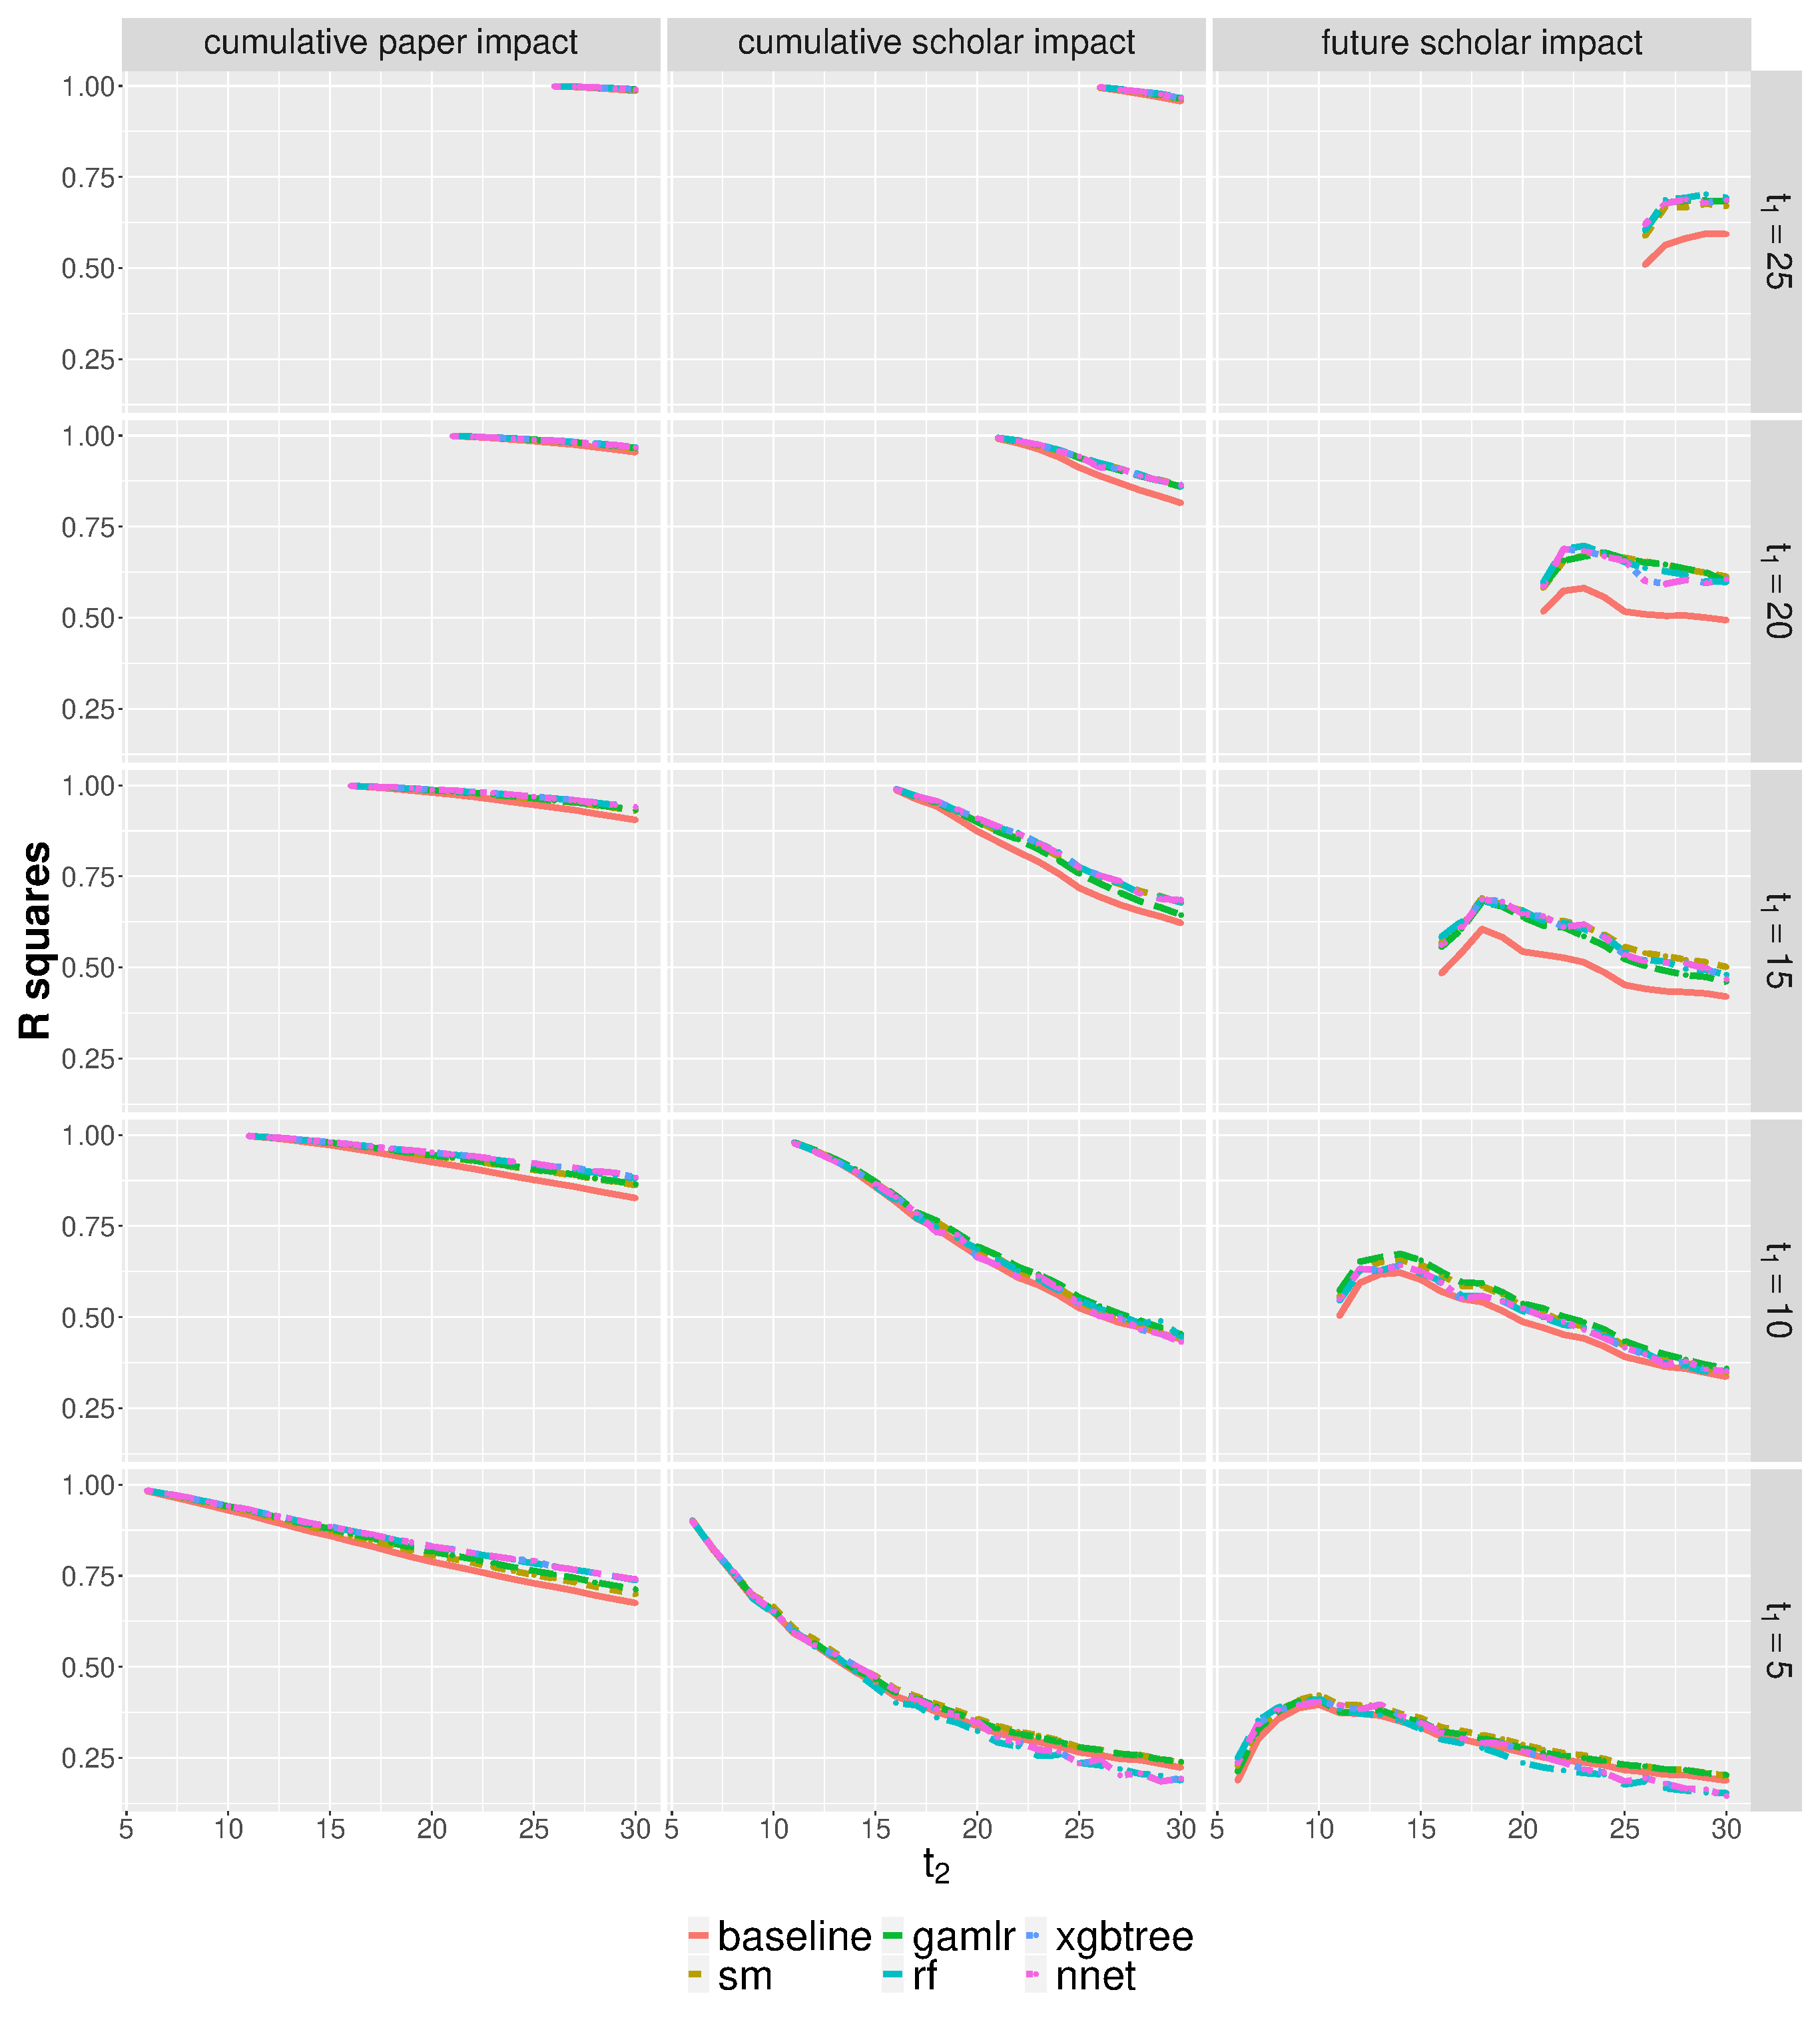
\includegraphics[width=\textwidth]{figures/pred_model/r2.eps}
    \caption[R squares of the predictive models]{Testing $R^2$ of the predictive models. The lasso, ridge, and elastic net are outperformed by the Gamma lasso and hence are ignored for a better visualization.}
    \label{fig:pred_r2}
\end{figure}







 %!TEX root = ms.tex
\section*{Discussion}

Rank percentile indicators compare the performance of a publication or a scholar relative to cohorts in the benchmark. They have the advantage of being interpretable and flexible in the choice of benchmark and evaluation metrics. We illustrate that the publication percentile is highly stable, while the scholar percentile exhibits short-term stability and can be predicted utilizing a simple linear regression model. In practice, the highly predictable rank percentiles can be utilized in combination with other metrics to picture the trajectory of a scholar or a publication and assist in academic decision making. 

%!TEX root = main.tex
\section*{Methods}
\noindent\textbf{Data description}
We focus on authors from all fields in the top universities across the States, who have a Google Scholar account by the end of year $2016$. The dataset includes the entire citation history for each publication of these authors. This gives us $14668$ authors in total, and together they contribute to more than $1.3$ million publications that receive around $100$ million citations in total. We've used the benchmark `biology' throughout our discussion. A scholar and all her corresponding publications are flagged as being in the field of biology, if the areas of interests that she lists on Google Scholar contain any of the keywords: `biology', `genetic', `neuroscience' and `cell'. An exploratory description of the dataset is shown in figure \ref{fig:exploratory}. 

\noindent\textbf{Training the machine learning methods}
All the methods are trained in \textit{R}\supercite{RCT2019} with the help of the package \textit{mlr}\supercite{Bischl2016}, which provides a pipeline of training, validating and testing the model. LASSO, ridge, elastic net, random forest and xgbtree are inbuilt learners of the package. Gamma LASSO and deep neural network are trained using packages \textit{gamlr}\supercite{taddy2017one} and \textit{keras}\supercite{Allaire2019} respectively.

All of the machine learning methods require the tuning of hyper-parameters. The process involves deciding the searching space of parameters and evaluating the sets of parameters using the validation data. The optimal model is the one that minimizes the validation error. Table \ref{tab:hyperpara} shows the hyper-parameter(s) for each machine learning model considered in this paper. It's worth noticing that the parameter space can be huge for method like xgbtree where we have an extensive list of tunable parameters. Randomized search with multiple iterations shall be preferred over the grid search in such scenario. Another choice can be using the Bayesian optimization that searches over the parameter space based on the performance gain. Meanwhile, parallel computing can further reduce the computing time.

The data and code are publicly available at \url{https://github.com/sentian/impact-ranking}. 








%\include{metrics}
%\include{pdmodel}
%\include{varmodel}
%%!TEX root = ms.tex
\section*{Calculation of the rank percentile indicator}

In this section, we start by discussing the framework for calculating the rank percentile indicator. For publications, the indicator is based on the number of citations. We further propose utilizing an aggregation of rank percentile indicators for publications as the evaluation metric, based on which we then construct the indicator for scholars. We discuss the advantage of the proposed indicator compared to indicator based on existing evaluation metrics, such as the number of citations or h-index. 

\subsection*{Dataset}

The dataset from Google Scholar includes scholars in multiple disciplines from the top $10$ universities in the United States, which totals $14358$ scholars. It includes the citation history through $2016$ for each publication from these scholars; they contributed to more than $800,000$ publications total, which received approximately $100$ million citations collectively. The discipline for a scholar is determined by the area of interest specified on the Google Scholar page. For instance, a scholar and his/her publications are labeled as in the area of biology if the area of interest contains any of the following keywords: biology, genetic, neuroscience, or cell. An exploratory description of the dataset can be found in Supplemental Material (Figure S5 and Table S4). The dataset and the code to reproduce the results in this paper are available online at \url{https://github.com/sentian/SciImpactRanking}.

\subsection*{Framework for calculating the rank percentile indicator}
Recall that the four fundamental elements for the rank percentile indicator are as follows. 
\begin{itemize}
    \item Entity: publication (P) or scholar (S).
    \item Benchmark (b): the reference set to which the entity is compared.
    \item Metric (m): the measure that evaluates the performance of the entity.
    \item Age (t): the time when the evaluation is executed.
\end{itemize}
The rank percentile for publication $j$, P$_{m}^{jb}(t)$, is calculated in the following way.

\begin{enumerate}[label=(\arabic*)]
    \item Evaluate the publications in the benchmark by their performance at age $t$ (publications with life shorter than $t$ are not included). Utilize the evaluation metric to calculate the rank r$_{m}^{jb}(t)$ of publication $j$ against the publications in the benchmark. An average rank is assigned to r$_{m}^{jb}(t)$ if there exist other publications that have the same value of the metric. 
    \item The rank percentile is indicated by $\text{P}_{m}^{jb}(t)= \left(\text{r}_{m}^{jb}(t)-0.5\right)/N$.
\end{enumerate}
With the compromise $0.5/N$ in the final step, the median paper is assigned $50\%$ percentile, and the tails of the citation distribution are treated symmetrically~\cite{allen1914storage}. The above framework can be easily adapted to compute the rank percentile indicators for scholar $i$: S$_{m}^{ib}(t)$.


\subsection*{The rank percentile indicator for scholars}

For publication $j$, we utilize the number of citations by age $t$ as the evaluation metric and denote the rank percentile indicator as P$_c^{jb}(t)$. We further utilize the publication indicators to construct the rank percentile for scholars. For scholar $i$, the performance is determined by the qualities of the scholar's publications, in which each publication is evaluated via P$_c^{jb}(5)$, meaning the rank percentile for the publication at the fifth year since published. The evaluation metric for scholar $i$ is determined by aggregating the performance of all $N(t)$ papers that the scholar publishes by age $t$, that is $\displaystyle \sum_{j=1}^{N(t)} \text{P}_c^{jb}(5)$. We denote the resulting rank percentile indicator as S$_{P5}^{ib}(t)$, where P5 indicates the evaluation metric based on rank percentile indicator of publications at age $5$. In the discussion that follows, we utilize the simplified notations P$_c$ and S$_{P5}$ to refer to the publication and scholar rank percentiles in general, respectively. 

Figure \ref{fig:auti} presents an example of S$_{P5}$ for a random scholar in our dataset in which the benchmark includes all tenured professors in the top 10 universities, as ranked by the U.S. News. The scholar's career started in 2004, and our dataset tracks the citation information until 2016. The indicator S$_{P5}$ ranks the scholar to be in the top $40\%$ throughout the majority of their career. The figure indicates two other types of rank percentile indicators, S$_c$ and S$_h$, that utilize the number of citations and h-index score as evaluation metrics, respectively. We see that S$_h$ largely agrees with S$_{P5}$, and S$_c$ ranks the scholar lower than the other two indicators. 

% fig:auti
% an example of the scholar RP
\begin{figure}[ht!]
    \centering
    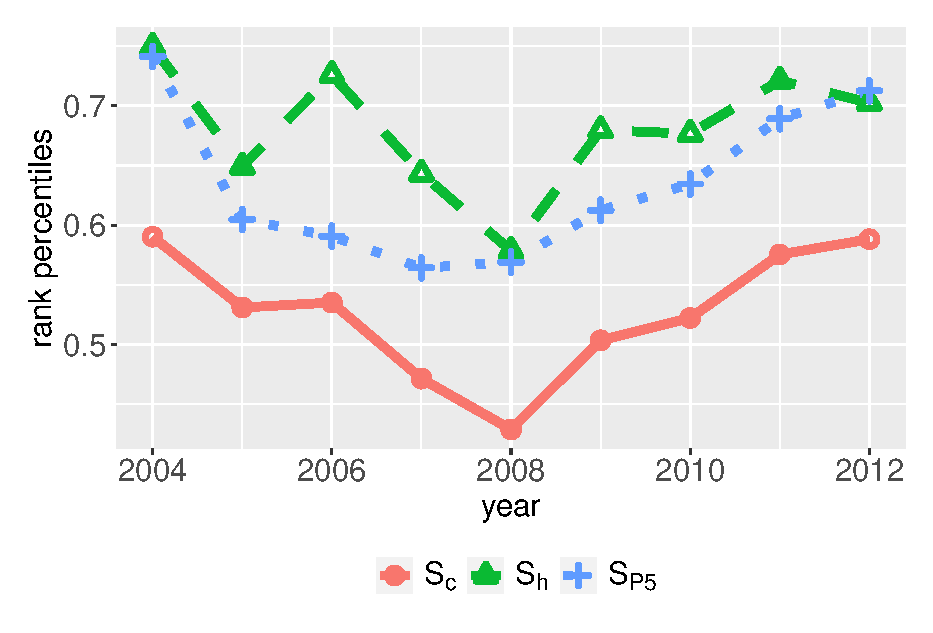
\includegraphics[width=0.6\textwidth]{figures/compare_autrp/auti.eps}
    \caption[rank percentile indicators for a random scholar]{The rank percentile indicators for a random scholar. The benchmark contains all tenured professors in the top-10 universities, as ranked by the U.S. News.}
    \label{fig:auti}
\end{figure}

The indicator S$_{P5}$ improves some major drawbacks of S$_c$ and S$_h$. First, it removes the seniority effect of publications. The evaluation metric for S$_c^{ib}(t)$ represents the citations that scholar $i$ receives by age $t$, which is the sum of citations for the scholar's publications by $t$. Compared to newly published works, publications with longer histories are more likely to attract citations and therefore contribute more to formulating S$_c$. A similar argument can be made for S$_h$. However, S$_{P5}$ treats the publications equally and evaluates them based on their performances at the publications' age of five. Additionally, a scholar who publishes a considerable number of low-impact works or participates in only a small number of high-impact projects can have a high value of S$_c$, since the absolute number of citations can be unlimited and is significantly influenced by extreme values. However, the S$_{P5}$ and S$_h$ of these scholars are not necessarily large, since these indicators limit the contribution of a single publication to be, at most, $1$ by definition of rank percentile and h-index score. Furthermore, compared to S$_h$, S$_{P5}$ penalizes scholars who are not truly innovative but carefully massage their h-index scores by publishing a number of papers that attract barely sufficient amounts of citations to increase their h-index scores. As long as a paper is among the top $h$ papers, the actual number of citations is irrelevant for h-index and S$_h$, but it can still impact S$_{P5}$. Finally, S$_{P5}$ requires less data compared to S$_c$ and S$_h$, since it only relies on the 5-year citation history of each publication. Hence, S$_{P5}$ is better suited to large-scale analysis.

We demonstrate the advantages of S$_{P5}$ by examining some extreme cases. We created three synthetic academic careers. Scholar A publishes a substantial number of publications throughout his/her career (more than $90\%$ of his/her cohorts in the benchmark), while all of the publications have little impact. Scholars B and C only publish one paper each at the beginning of their careers; B's paper is astonishing, while C's paper is average. Both scholars have an h-index equal to $1$ throughout their careers. Figure \ref{fig:simulated_authors} illustrates the rank percentile indicators for these three artificial scholars. We see that flooding low-impact publications can increase S$_c$ at the beginning of Scholar A's career. We also see that a single high-impact work improves the value S$_c$ throughout Scholar B's career; the author remains in the top $50\%$ at age $12$, as indicated by S$_c$. Both S$_{P5}$ and S$_h$ better characterize the performances of these authors. Finally, S$_h$ remains the same for Scholars B and C since they each have an h-index of $1$ throughout their careers. However, S$_{P5}$ considers that Scholar B's publication has a greater impact and therefore ranks higher than Scholar C. 

% fig:simulated_authors
% show the difference between various author rp
\begin{figure}[ht!]
    \centering
    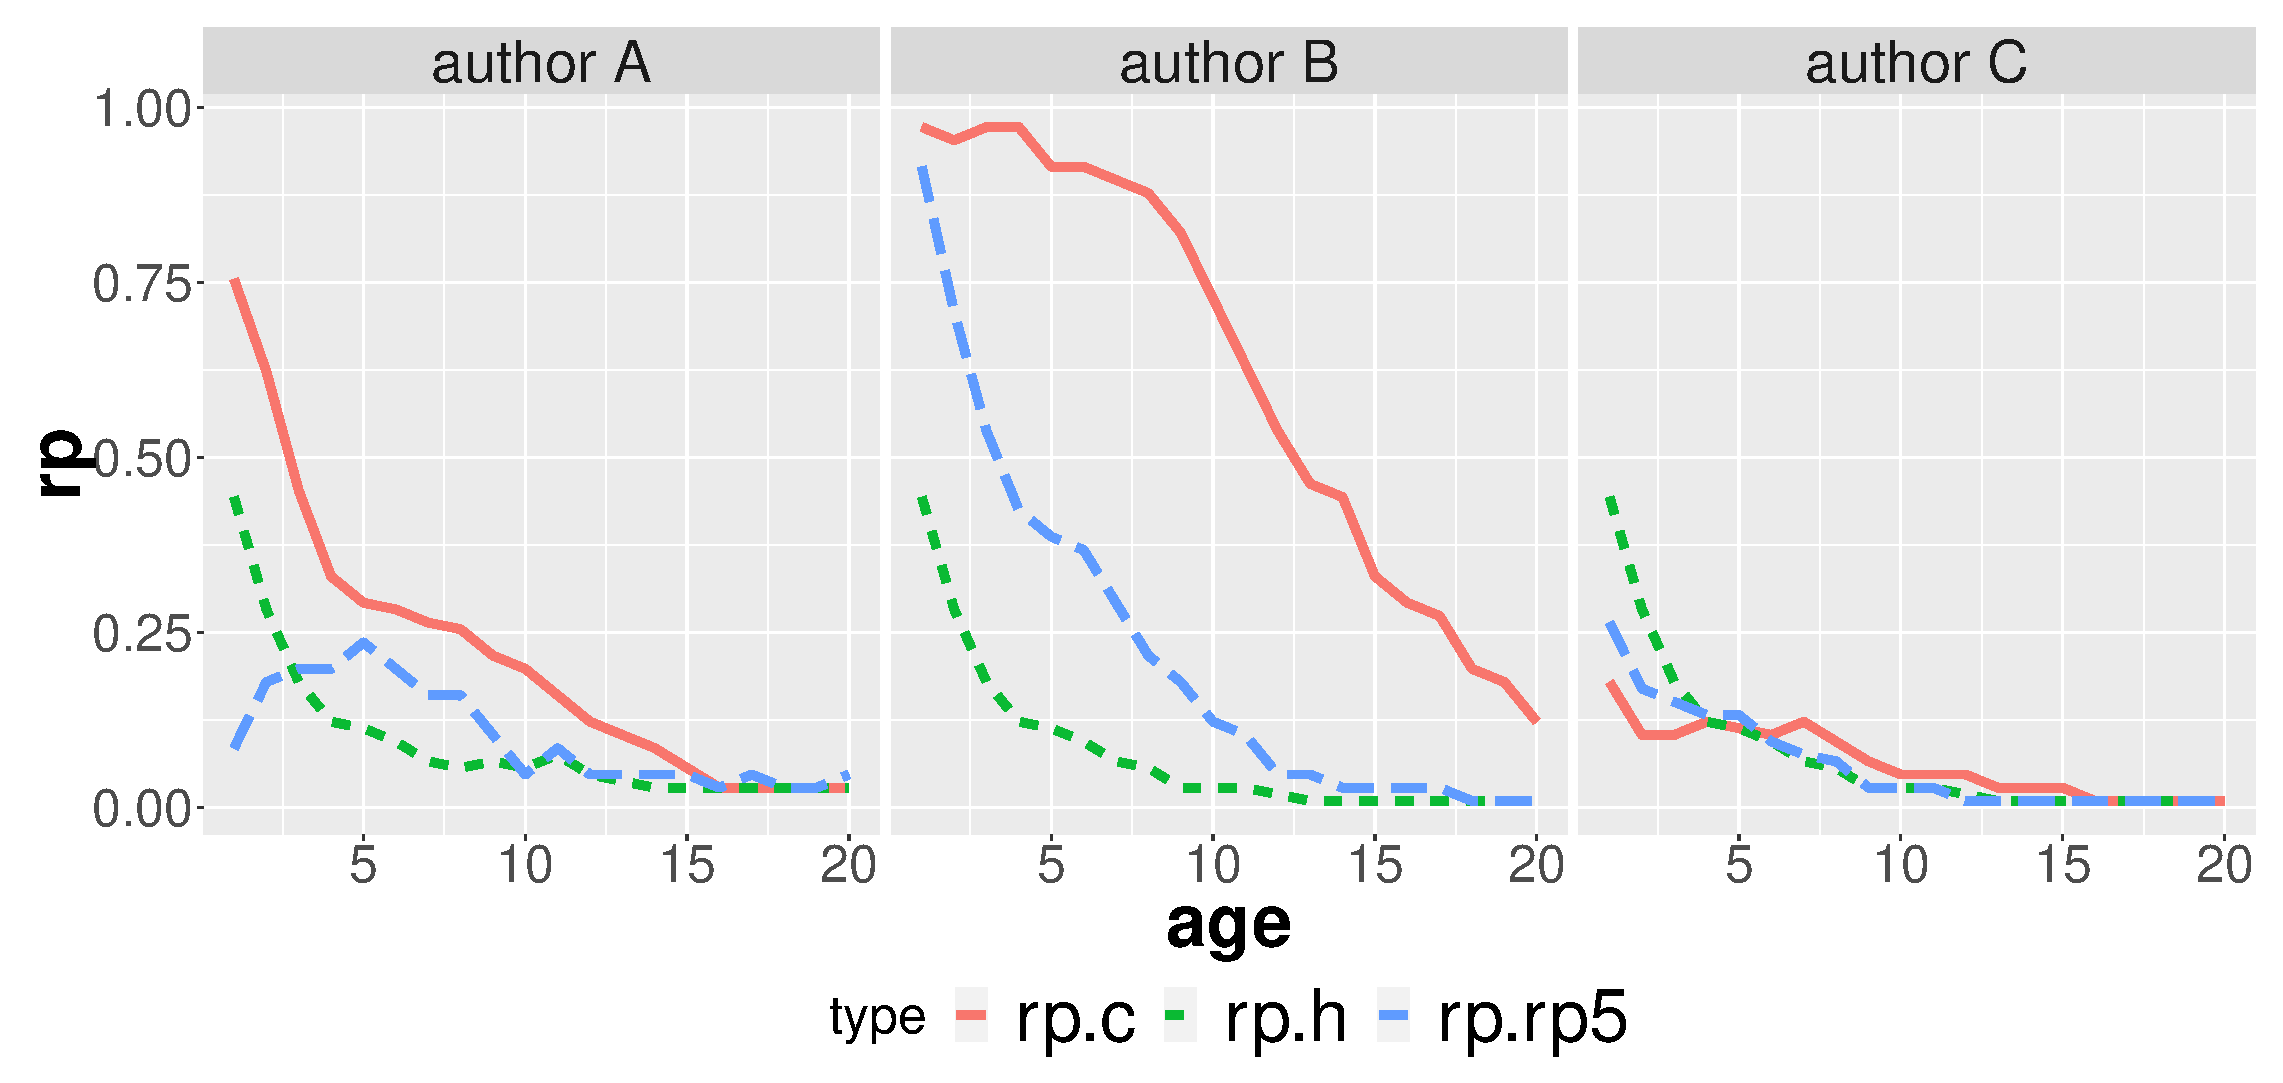
\includegraphics[width=\textwidth]{figures/compare_autrp/simulated_authors.eps}
    \caption[The advantage of S$_{it}^{P5}$ compared to other indicators]{Three artificial scholars illustrate the difference between various types of rank percentile indicators for scholars. Scholar A is highly productive at all ages, but all of the works have little impact. Scholars B and C only publish one paper each at age $1$; the paper of Scholar B has substantial impact, while the paper of Scholar C has medium impact. The h-index scores of Scholars B and C remain at $1$ throughout their careers. The benchmark includes scholars in biology who started their careers in $1990$.}
    \label{fig:simulated_authors}
\end{figure}

With the exception of the above-mentioned discrepancies, we present in Supplemental Material Section \ref{sec:suppl_similarity_autrp} that for the majority of scholars in our dataset, S$_{P5}$ largely agrees with S$_c$ and S$_h$. Furthermore, we consider utilizing various metrics to evaluate the publication, for example P$_c^{jb}(10)$ which is based on 10-year citation history. As we reveal Supplemental Material Section \ref{sec:suppl_robustness_P5}, the differences between the resultant rank percentile indicators and S$_{P5}$ are not statistically significant, thus indicating the robustness of S$_{P5}$. Intuitively, the publication percentile P$_c^{jb}(t)$ is highly stable over $t$, and therefore P$_c^{jb}(5)$ can be a reasonable indicator of the performance for the publication. The details will be discussed in the next section.

\section*{The predictability of rank percentile indicator}

In this section, we study the predictability of the rank percentile indicator. In general, we find the indicator to exhibit stability over time, and the indicator can be predicted via some simple linear regression models. 

\subsection*{The stationarity of the rank percentile indicator for scholars}

In the example of the tenure promotion, we utilized the rank percentile to compare the candidate with senior cohorts. The comparison is not valid if the candidate is more likely to attract citations than senior colleagues who started their careers years earlier. In such a case, it may well be the academic environment that results in a better performance of the candidate rather than the internal factors, such as creativity and productivity.

Figure \ref{fig:rp_stationarity} portrays S$_{P5}$ at age $10$, grouped by the starting year of academic careers. We see that S$_{P5}$ does not exhibit an obvious trend and is approximately stationary over the starting year of careers, thus providing empirical evidence for the validity of the rank percentile. 

\begin{figure}[ht!]
    \centering
    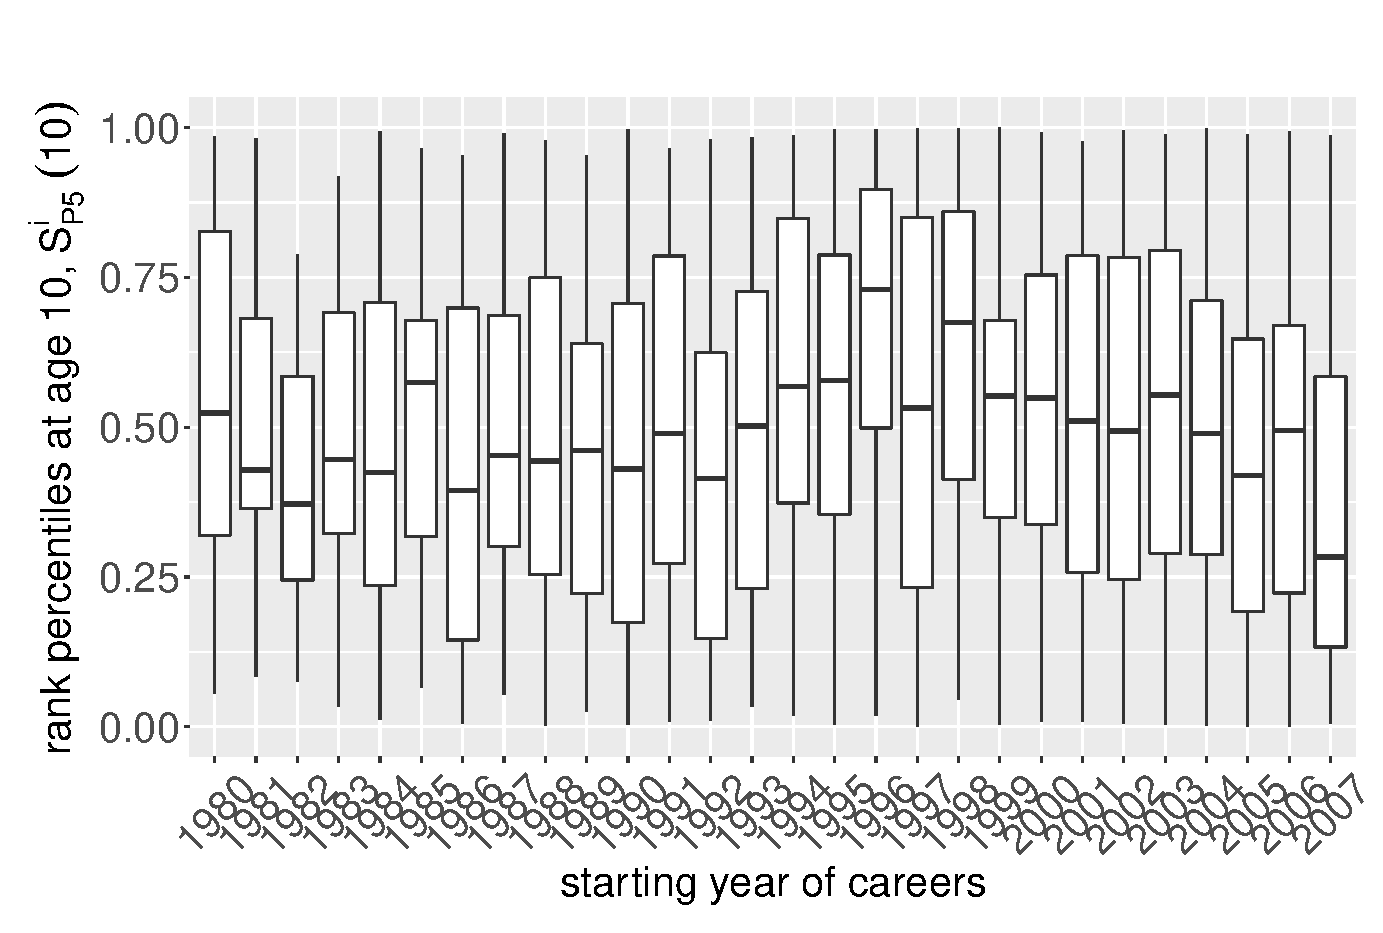
\includegraphics[width=0.6\textwidth]{figures/stationarity/rp_stationarity.eps}
    \caption[Stationarity of rank percentile indicators]{S$_{P5}(10)$ grouped by the starting years of academic careers. The benchmark contains all tenured professors in the top-10 universities, as ranked by the U.S. News.} 
    \label{fig:rp_stationarity}
\end{figure}

\subsection*{The predictability of rank percentile indicator}

Citations have been proven to lack long-term predictive power~\cite{Wang2013}. Figure \ref{fig:pred_cit_age} illustrates that papers with the same citations by the fifth year since published can have noticeably different citation paths and long-term effects. Additionally, exceptional and creative ideas typically require a lengthy period to be appreciated by the scientific community. As presented in Figure \ref{fig:pred_cit_cit}, the correlation between short- and long-term citations breaks down for the most highly-cited publications (the shaded rectangle). These problems can be largely avoided by utilizing rank percentile indicators, as evidenced in Figures \ref{fig:pred_rp_age} and \ref{fig:pred_rp_rp}. The considerable variation in the long-term effect of citations is restricted by utilizing rank percentiles. For publications with high impact, the correlation between short- and long-term effects persists when utilizing rank percentiles.

% publication rank percentile vs citations, predictability, Wang(2013)
\begin{figure}[ht!]
    \centering
    \begin{subfigure}[b]{0.48\textwidth}
     \centering
     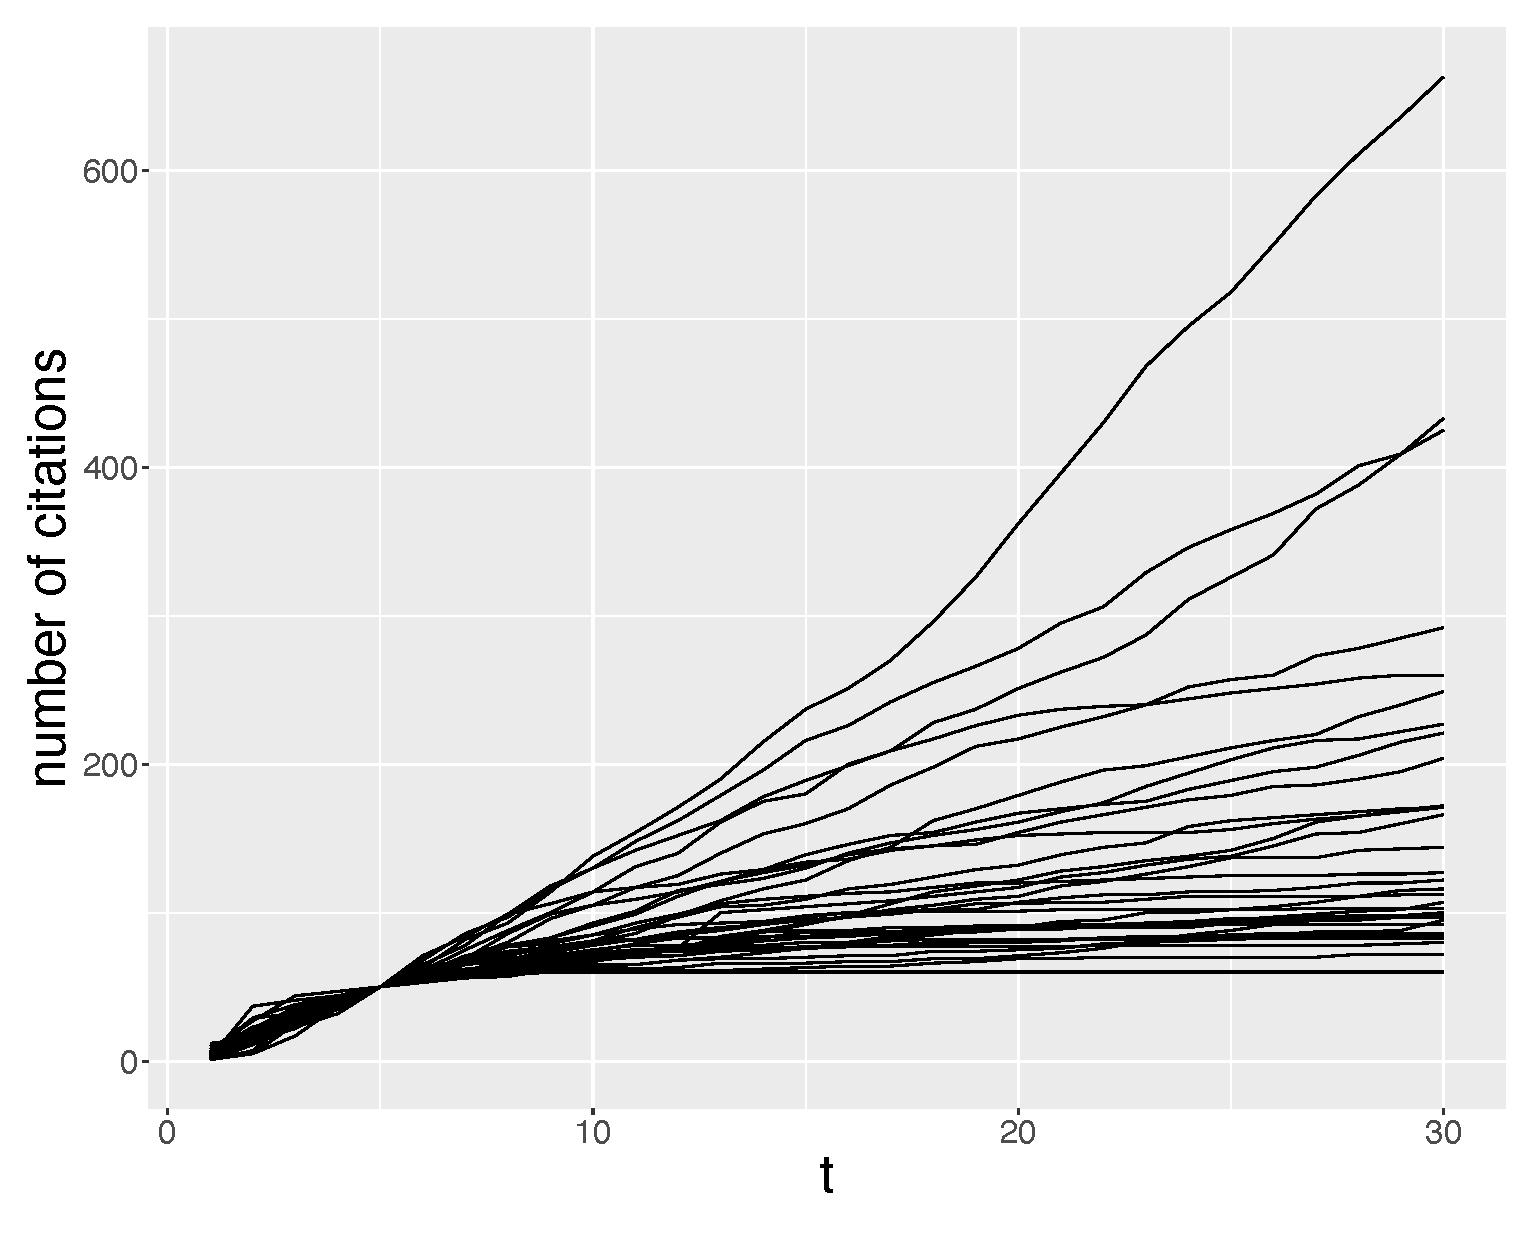
\includegraphics[width=\textwidth]{figures/pred_power/cit_t.eps}
     \caption{Number of citations versus age}
     \label{fig:pred_cit_age}
    \end{subfigure}
    \hfill
    \begin{subfigure}[b]{0.48\textwidth}
     \centering
     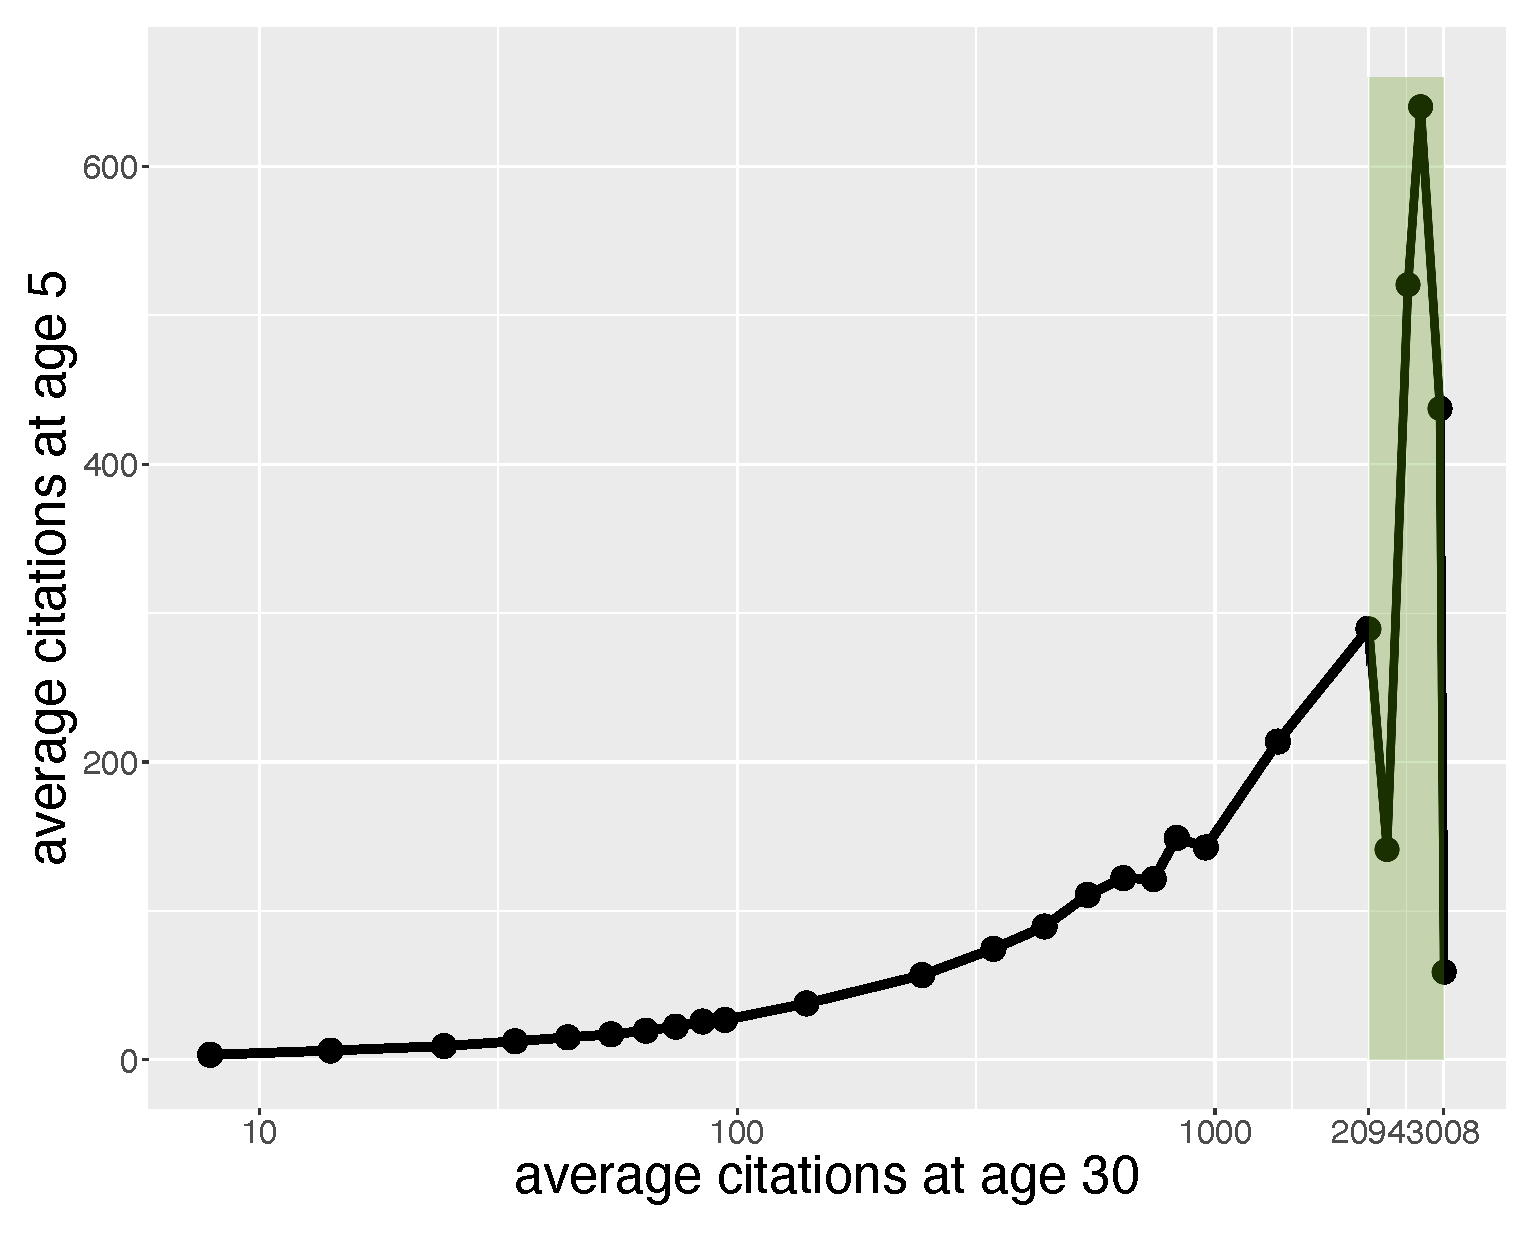
\includegraphics[width=\textwidth]{figures/pred_power/cit_cit.eps}
     \caption{Average citations at age $5$ versus those at age $30$}
     \label{fig:pred_cit_cit}
    \end{subfigure}
    \caption[Predictability of citations]{The predictability of citations. The benchmark contains the publications in biology. Figure \ref{fig:pred_cit_age} portrays the cumulative citations for publications that have $50$ citations by the fifth year since published. Figure \ref{fig:pred_cit_cit} displays the average citations by age $5$ versus the average citations by age $30$. The averages are calculated over groups of publications, which are prespecified by dividing the range of citations by age $30$ into equal intervals on the log scale. Note that we do not claim the originality of the figures, which have been illustrated via a different dataset~\cite{Wang2013}.}
    \label{fig:pub_cit_pred}
\end{figure}


\begin{figure}[ht!]
    \centering
    \begin{subfigure}[b]{0.495\textwidth}
     \centering
     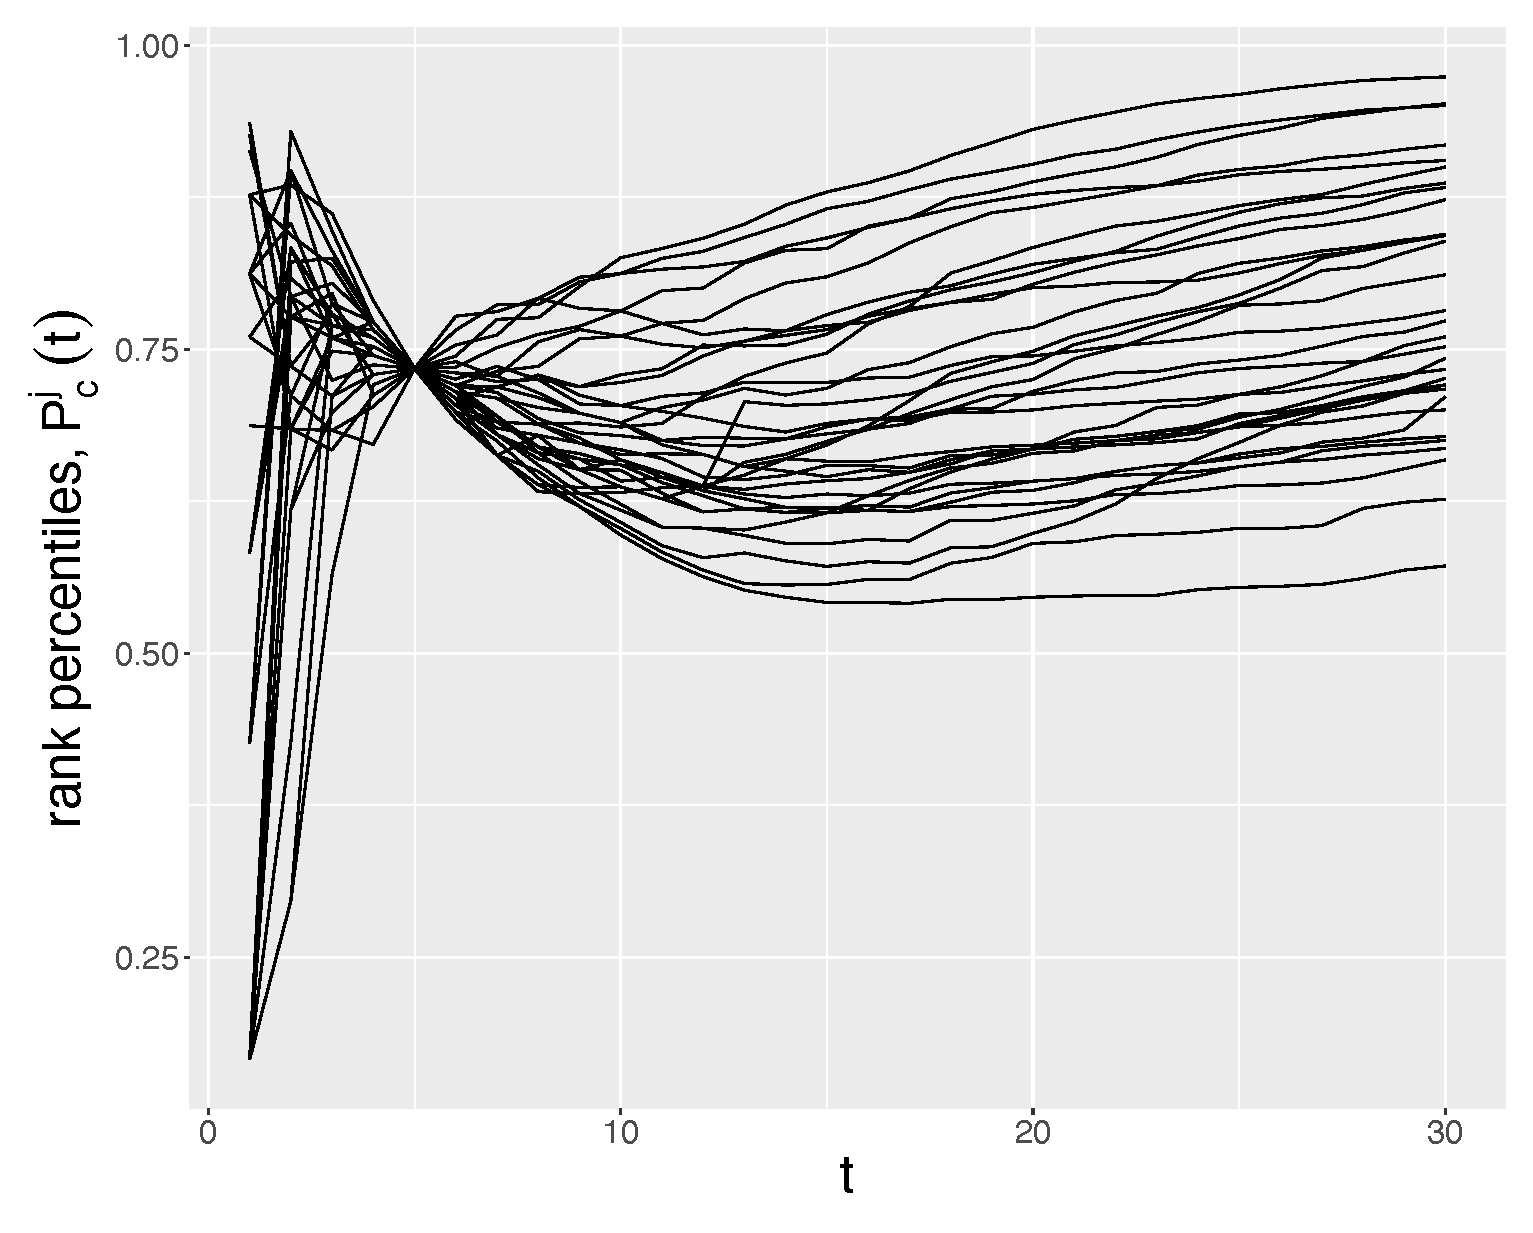
\includegraphics[width=\textwidth]{figures/pred_power/rp_t.eps}
     \caption{Rank percentiles P$_c$ versus age}
     \label{fig:pred_rp_age}
    \end{subfigure}
    \hfill
    \begin{subfigure}[b]{0.495\textwidth}
     \centering
     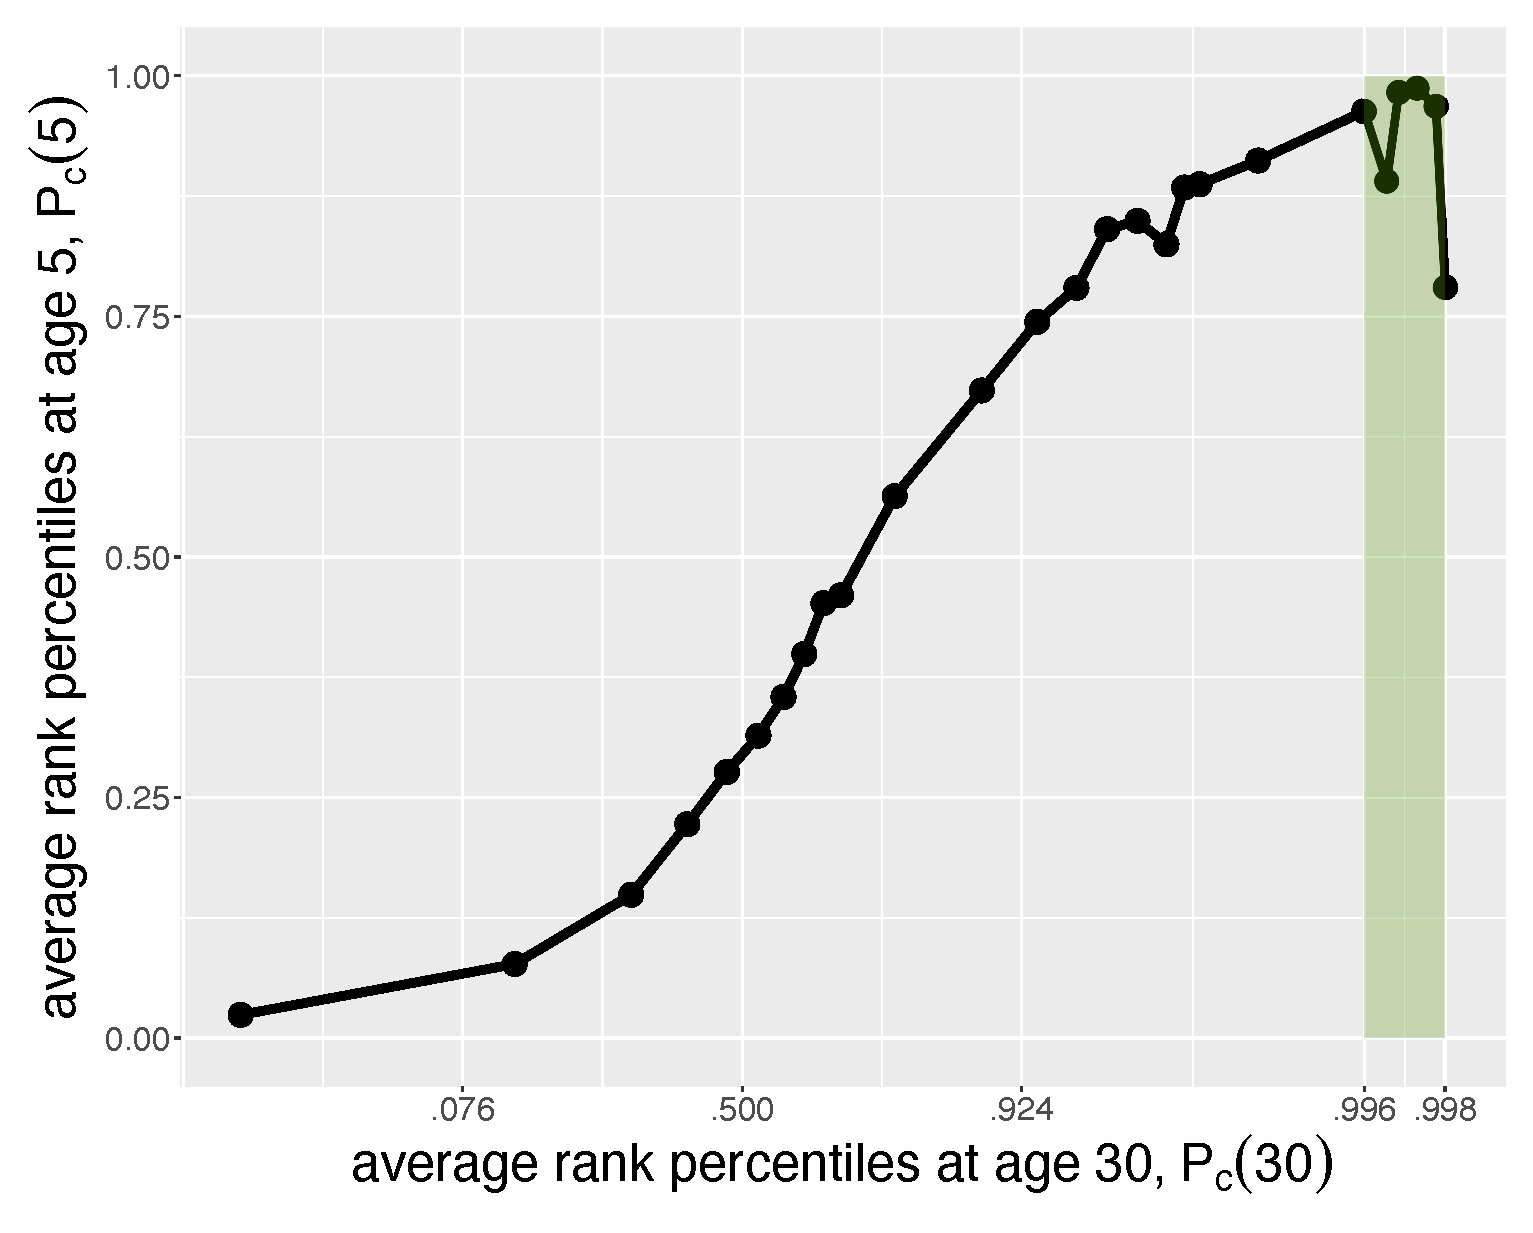
\includegraphics[width=\textwidth]{figures/pred_power/rp_rp.eps}
     \caption{Average P$_c$ at age $5$ versus those at age $30$}
     \label{fig:pred_rp_rp}
    \end{subfigure}
    \caption[Predictability of rank percentiles]{The predictability of rank percentiles. Figure \ref{fig:pred_rp_age} demonstrates the rank percentiles for the publications considered in Figure \ref{fig:pred_cit_age}. Figure \ref{fig:pred_rp_rp} presents the average of P$_c(5)$ versus the average of P$_c(30)$ for the same groups of publications as in Figure \ref{fig:pred_cit_cit}.}
    \label{fig:pub_rp_pred}
\end{figure}

We further characterize the predictability of rank percentile indicators. Figure \ref{fig:hm_rp_pub} presents the correlation between rank percentiles at two ages, P$_c^{jb}(t_1)$ and P$_c^{jb}(t_2)$ where $t_1<t_2$. We noticed overall large correlations for both benchmarks. The correlation diminishes as the forecast horizon $(t_2-t_1)$ increases, which simply reflects the difficulty of long-term forecasting. Additionally, the correlation increases as $t_1$ increases while holding the forecast horizon fix. This indicates that the performance of a senior publication is easier to predict, since the longer history removes more uncertainties regarding its performance. We further noticed a slightly higher predictive power when we restricted the benchmark to be the area of biology. 

Figure \ref{fig:hm_rp_aut} illustrates that the patterns discussed above generally hold for rank percentiles of scholars. The magnitude of correlations is smaller than those for publications, especially for long-term forecasts. This results from the fact that forecasting the future impact of future works is considerably more difficult than forecasting the future impact of existing works. Intuitively, predicting S$_{P5}^{ib}(t_2)$ involves predicting the performance of papers published before $t_1$ and predicting the performance of those published between $t_1$ and $t_2$. The former is predicting the future impact of existing works, while the latter is predicting the future impact of future works. However, predicting the publication indicator P$_c^{jb}(t_2)$ only involves predicting the future impact of publication $j$, which is a considerably easier task. Furthermore, when the forecast horizon increases while fixing $t_1$, additional future works are involved in predicting S$_{P5}^{ib}(t_2)$; therefore, we see that the correlation decreases more quickly than when we predict P$_c^{jb}(t_2)$. 

% publication rank percentile, heat map of correlations
\begin{figure}[ht!]
    \centering
    \begin{subfigure}[b]{0.8\textwidth}
        \centering
             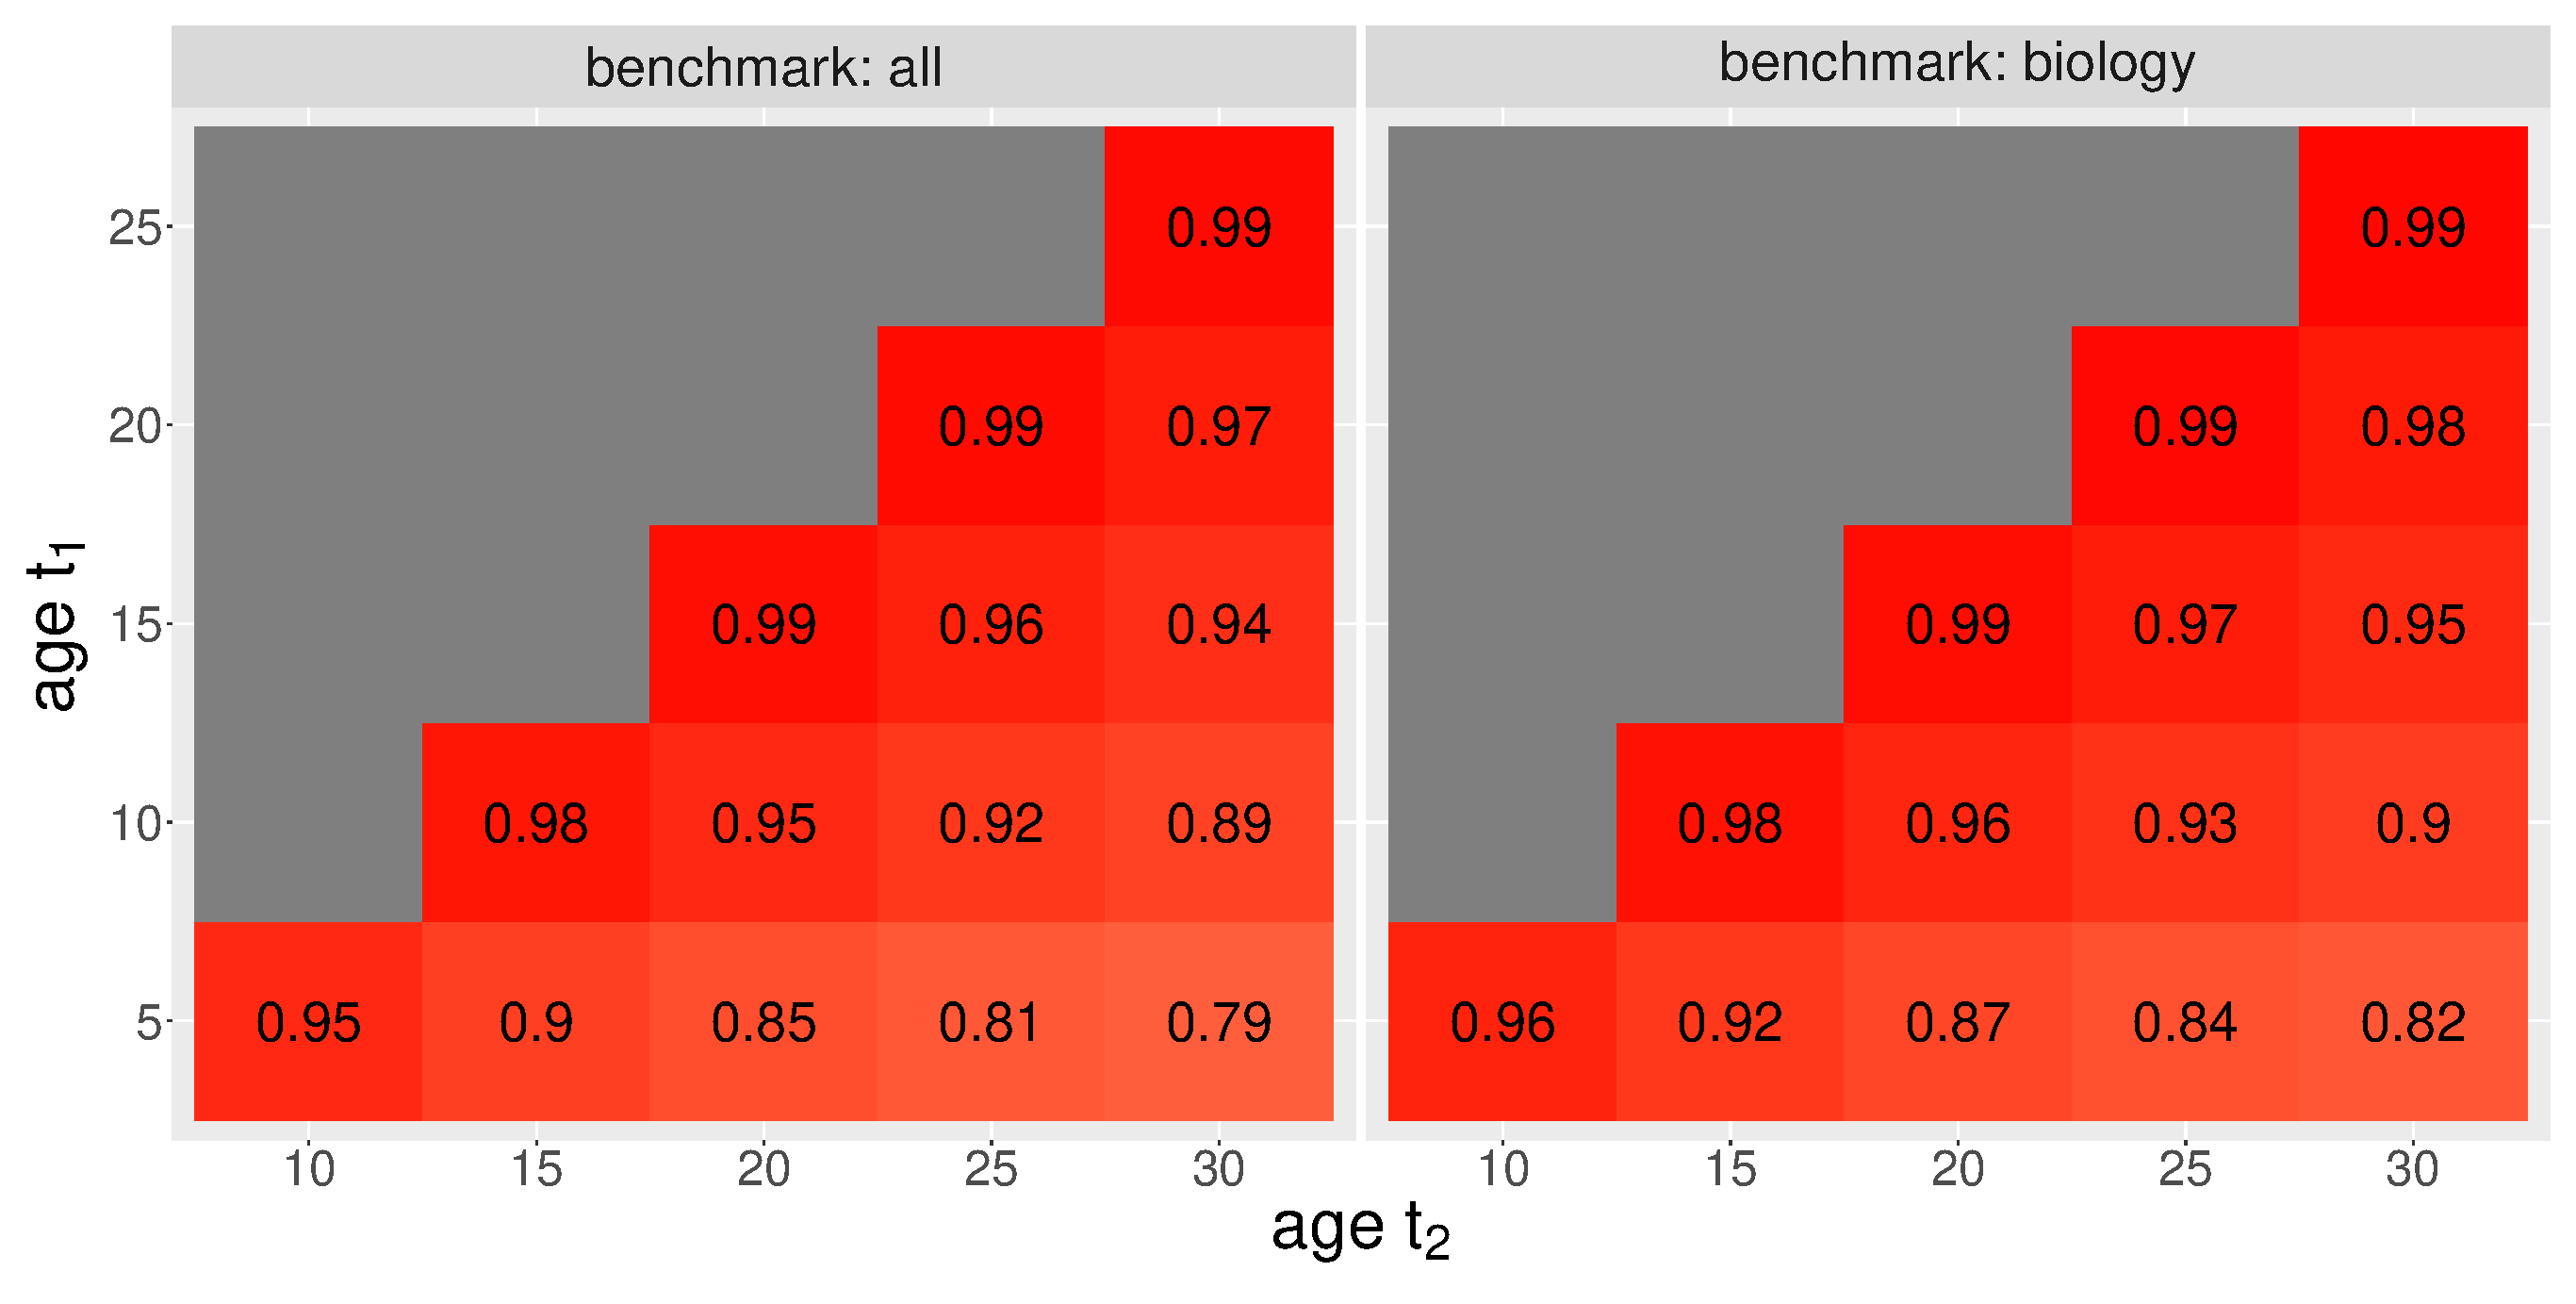
\includegraphics[width=\textwidth]{figures/pred_power/heatmap_cor_pub.eps}
         \caption{Correlation between P$_c^{jb}(t_1)$ and P$_c^{jb}(t_2)$}
         \label{fig:hm_rp_pub}
    \end{subfigure}

    \begin{subfigure}[b]{0.8\textwidth}
        \centering
             \includegraphics[width=\textwidth]{figures/pred_power/heatmap_cor_aut.eps}
         \caption{Correlation between S$_{P5}^{ib}(t_1)$ and S$_{P5}^{ib}(t_2)$}
         \label{fig:hm_rp_aut}
    \end{subfigure}

    \begin{subfigure}[b]{0.8\textwidth}
        \centering
             \includegraphics[width=\textwidth]{figures/pred_power/heatmap_cor_aut_future.eps}
         \caption{Correlation between S$_{P5}^{ib}(t_1)$ and S$_{P5}^{ib}(t_2 | t_1)$}
         \label{fig:hm_rp_aut_future}
    \end{subfigure}
    \caption[Correlations between rank percentiles at different ages]{The Pearson's correlation between rank percentile indicators at two different ages. }
    \label{fig:hm_rp}
\end{figure}

\begin{figure}[ht!]
    \centering
    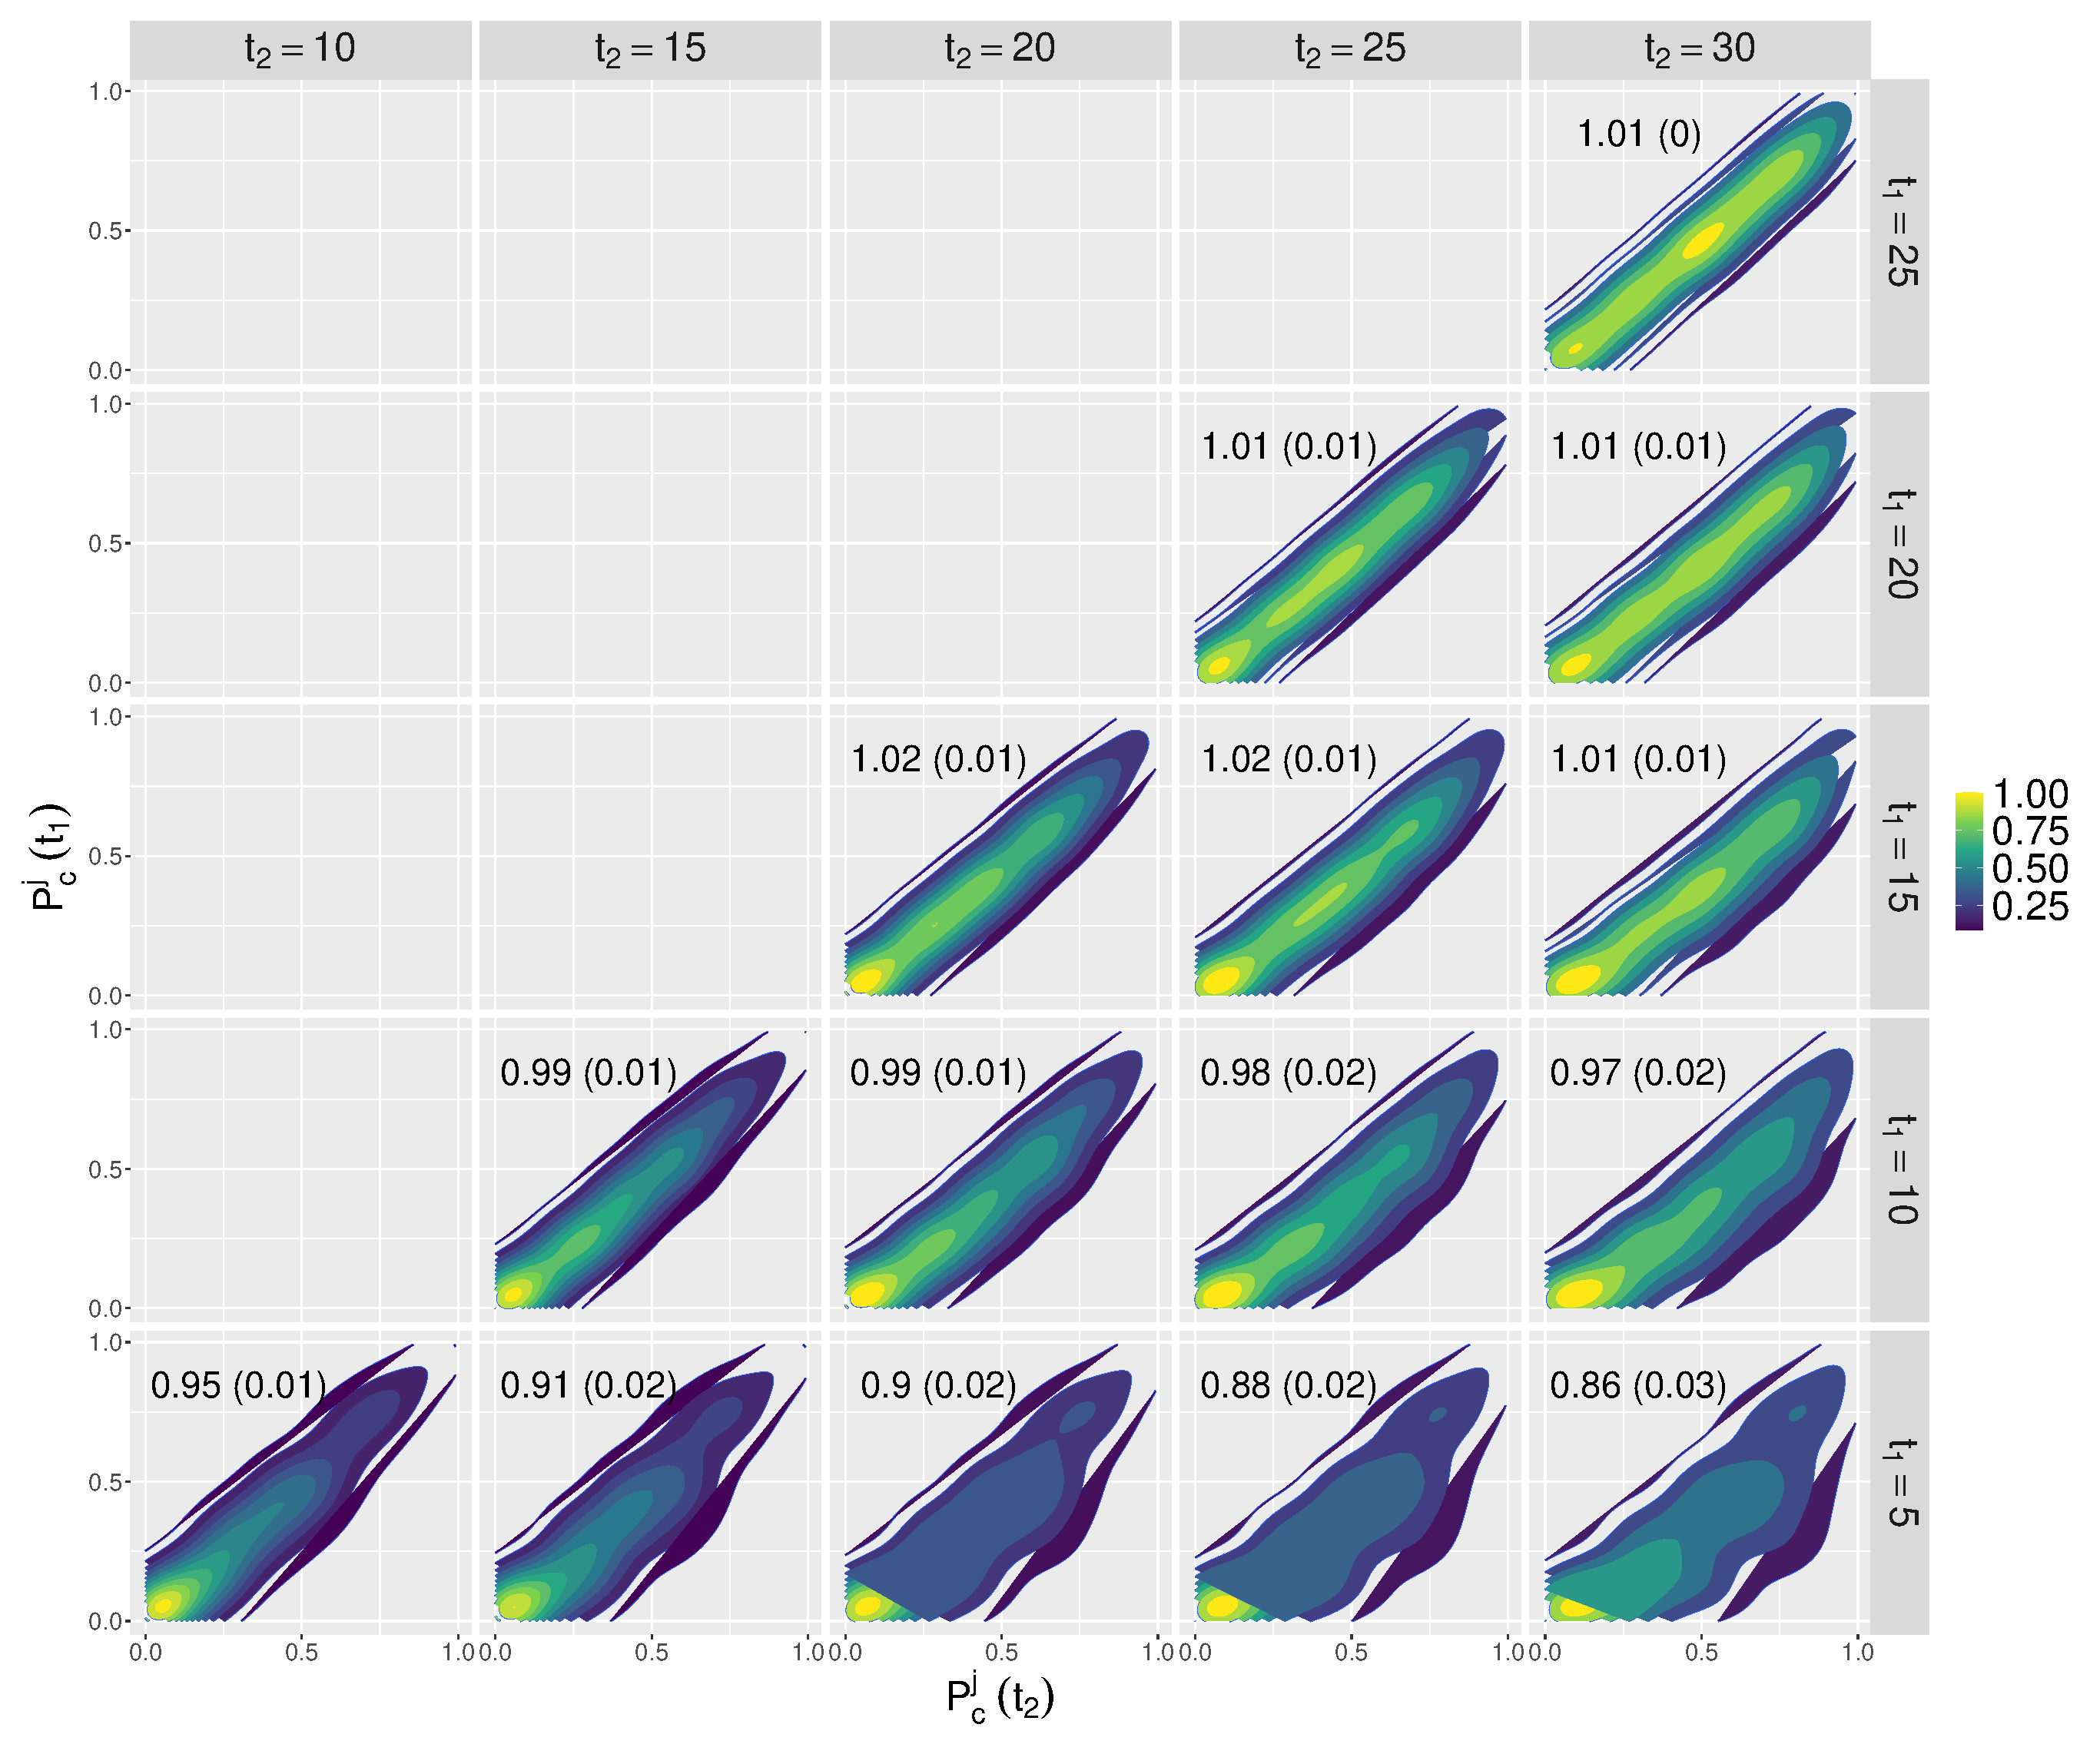
\includegraphics[width=\textwidth]{figures/pred_power/scatter_pubrp_bio1980.eps}
    \caption[Kernel density estimation for the scatter points of P$_c(t_1)$ and P$_c(t_2)$]{Kernel density estimation for the scatter points of P$_c^{jb}(t_1)$ and P$_c^{jb}(t_2)$. We also fitted a simple linear regression of P$_c^{jb}(t_2)$ on P$_c^{jb}(t_1)$. The estimated coefficient and the corresponding standard error (in parentheses) are displayed in each plot. The benchmark here includes publications in biology that were published in $1980$.}
    \label{fig:scatter_pubrp_bio1980}
\end{figure}


The strong linear relationship between P$_{c}^{jb}(t_1)$ and P$_c^{jb}(t_2)$ is further characterized in Figure \ref{fig:scatter_pubrp_bio1980}. The data are along the $45 \degree$ line, and the linear regression coefficient of P$_c^{jb}(t_2)$ on P$_c^{jb}(t_1)$ is close to $1$ with small standard errors, thus indicating the high stability of P$_c$. A similar figure for S$_{P5}$ is displayed in Supplemental Material Figure \ref{fig:scatter_autrp_all}, in which we find that S$_{P5}$ exhibits short-term stability.

Predicting S$_{P5}^{ib}(t_2)$ can assist in decision making for faculty positions or granting tenure, since the committee would like to examine the cumulative scientific impact of the scholar. In assigning research funding or allocating research resources regarding planned studies and potential future publications, the future impact of future works is often of interest. We utilize S$_{P5}^{ib}(t_2|t_1)$ to denote the rank percentile indicator calculated based on papers published between $t_1$ and $t_2$. Figure \ref{fig:hm_rp_aut_future} illustrates the correlation between S$_{P5}^{ib}(t_1)$ and S$_{P5}^{ib}(t_2|t_1)$. The magnitudes of correlation are moderately high, indicating an approximately linear relationship, although the strength is not as strong as it was in predicting the cumulative impact, that is, predicting S$_{P5}^{ib}(t_2)$, which is consistent with our expectation.

\subsection*{Predictive models}
We now formulate the prediction tasks as supervised learning problems, and we illustrate that the rank percentile indicators can be predicted via simple linear models. We consider the following fitting procedures; these models are ordered by increasing complexity:
\begin{itemize}
    \item Baseline: simple linear regression model.
    \item Simple Markov model (sm).
    \item Penalized linear regression models, including the ridge~\cite{hoerl1970ridge}, lasso~\cite{Tibshirani1996}, elastic net (enet)~\cite{zou2005regularization} and the Gamma lasso (gamlr)~\cite{Taddy2017}.
    \item Ensemble methods of regression trees, including the random forest (rf)~\cite{liaw2002classification} and extreme gradient boosting trees (xgbtree)~\cite{chen2016xgboost}.
    \item Neural networks (nnet).
\end{itemize}

The baseline model fits a simple linear regression of the target variable on the autoregressive feature, e.g. P$_c^{jb}(t_1)$ for predicting the publication impact. The simple Markov model further considers the change of the autoregressive feature in the past two ages, e.g. P$_c^{jb}(t_1)$-P$_c^{jb}(t_1-2)$, in addition to the autoregressive feature and fits a linear regression model. 

\subsubsection*{Features and model fitting}

For the rest of the methods, we created an extensive list of features based on the citation histories. The features are characterized as either scholar- or publication-based features. For example, to predict the scholar indicator S$_{P5}^{ib}(t_2)$, a scholar-based feature is the number of papers that scholar $i$ publishes by age $t_1$, and a publication-based feature is the average number of citations for these papers. We established a total of $30$ features for predicting the publication indicator and $42$ features for predicting the scholar indicator, which can be found in the Supplemental Material Tables \ref{tab:features_pubrp} and \ref{tab:features_autrp}, respectively. Note that many of the features have been utilized when formulating the prediction task for number of citations and h-index scores~\cite{acuna2012future,weihs2017learning}.

The features were created utilizing the citation information available by $t_1$, and the dependent variable was specified at $t_2$. The data was split into the training and testing set based on a 9:1 ratio. We considered five stages of a publication or a scholar, that is, $t_1\in\{5,10,15,20,25\}$, and we forecasted up to $30$ years of age, that is, $t_2=t_1+1,\cdots,30$; this resulted in $75$ pairs of $(t_1,t_2)$ in total. The models were independently trained $75$ times. 

We also noted (in the Supplemental Material Section \ref{sec:suppl_stationarity}) that both S$_{P5}$ and P$_c$ are non-stationary time series, as evidenced by the Dicky-Fuller test~\cite{dickey1979distribution} and the KPSS test~\cite{kwiatkowski1992testing}. The differenced series are stationary (also presented in the Supplemental Material) and are utilized as the response variable, that is $\Delta \text{P}_{c}^{jb}(t_2) = \text{P}_{c}^{jb}(t_2) - \text{P}_{c}^{jb}(t_1)$, $\Delta \text{S}_{P5}^{ib}(t_2) = \text{S}_{P5}^{ib}(t_2) - \text{S}_{P5}^{ib}(t_1)$, and $\Delta \text{S}_{P5}^{ib}(t_2|t_1) = \text{S}_{P5}^{ib}(t_2|t_1) - \text{S}_{P5}^{ib}(t_1)$. Note that the stationarity discussed here characterizes the property of S$_{P5}$ and P$_c$ as time series. It is different from the stationarity as discussed in Figure \ref{fig:rp_stationarity}, where we fix $t=10$ and examine the stationarity of S$_{P5}(10)$ over the starting year of the scholars' careers.

The machine learning methods were trained using \textit{R}~\cite{RCT2019} with the package \textit{mlr}~\cite{Bischl2016}, which provides a pipeline of training, validating, and testing for the model. The lasso, ridge, elastic net, random forest, and xgbtree are inbuilt learners of the package. The Gamma lasso and neural network were trained utilizing \textit{R} packages \textit{gamlr}~\cite{Taddy2017} and \textit{keras}~\cite{Allaire2019}, respectively. 

The machine learning methods require hyperparameter tuning, which involves deciding the search space of parameters and evaluating the sets of parameters utilizing the validation data. The optimal model is the one that minimizes the validation error. The hyperparameters for each machine learning model considered in this paper are presented in Supplemental Material Table \ref{tab:hyperpara}. The parameter space can be substantial for methods such as xgbtree, which utilizes an extensive list of tunable parameters. We applied Bayesian optimization, which searches over the parameter space based on the performance gain.


\subsubsection*{Results}

The prediction accuracy is presented in Figure \ref{fig:pred_r2}. We see 
that the baseline model predicts the cumulative impacts, P$_c^{jb}(t_2)$ and S$_{P5}^{ib}(t_2)$, well, and the usage of a large number of features and complex machine learning models offers little improvement. Predicting the future impact of scholars, S$_{P5}^{ib}(t_2|t_1)$, is more difficult. The baseline model can still provide reasonable predictions, but the performance is not as satisfactory as others, especially when $t_1$ is large. By simply adding the difference $\text{S}_{P5}^{ib}(t_1) - \text{S}_{P5}^{ib}(t_1-2)$ as an extra feature, the simple Markov model achieves similar performance compared to the complex machine learning models, which rely on an extensive list of features and exhibit non-linear relationships. Other types of evaluation metrics for the predictive models, including the root mean squared error, root median squared error, and mean absolute error, can be found in the Supplemental Material (Figures \ref{fig:pred_rmse}, \ref{fig:pred_medse}, and \ref{fig:pred_mae}, respectively). 

\begin{figure}[ht!]
    \centering
    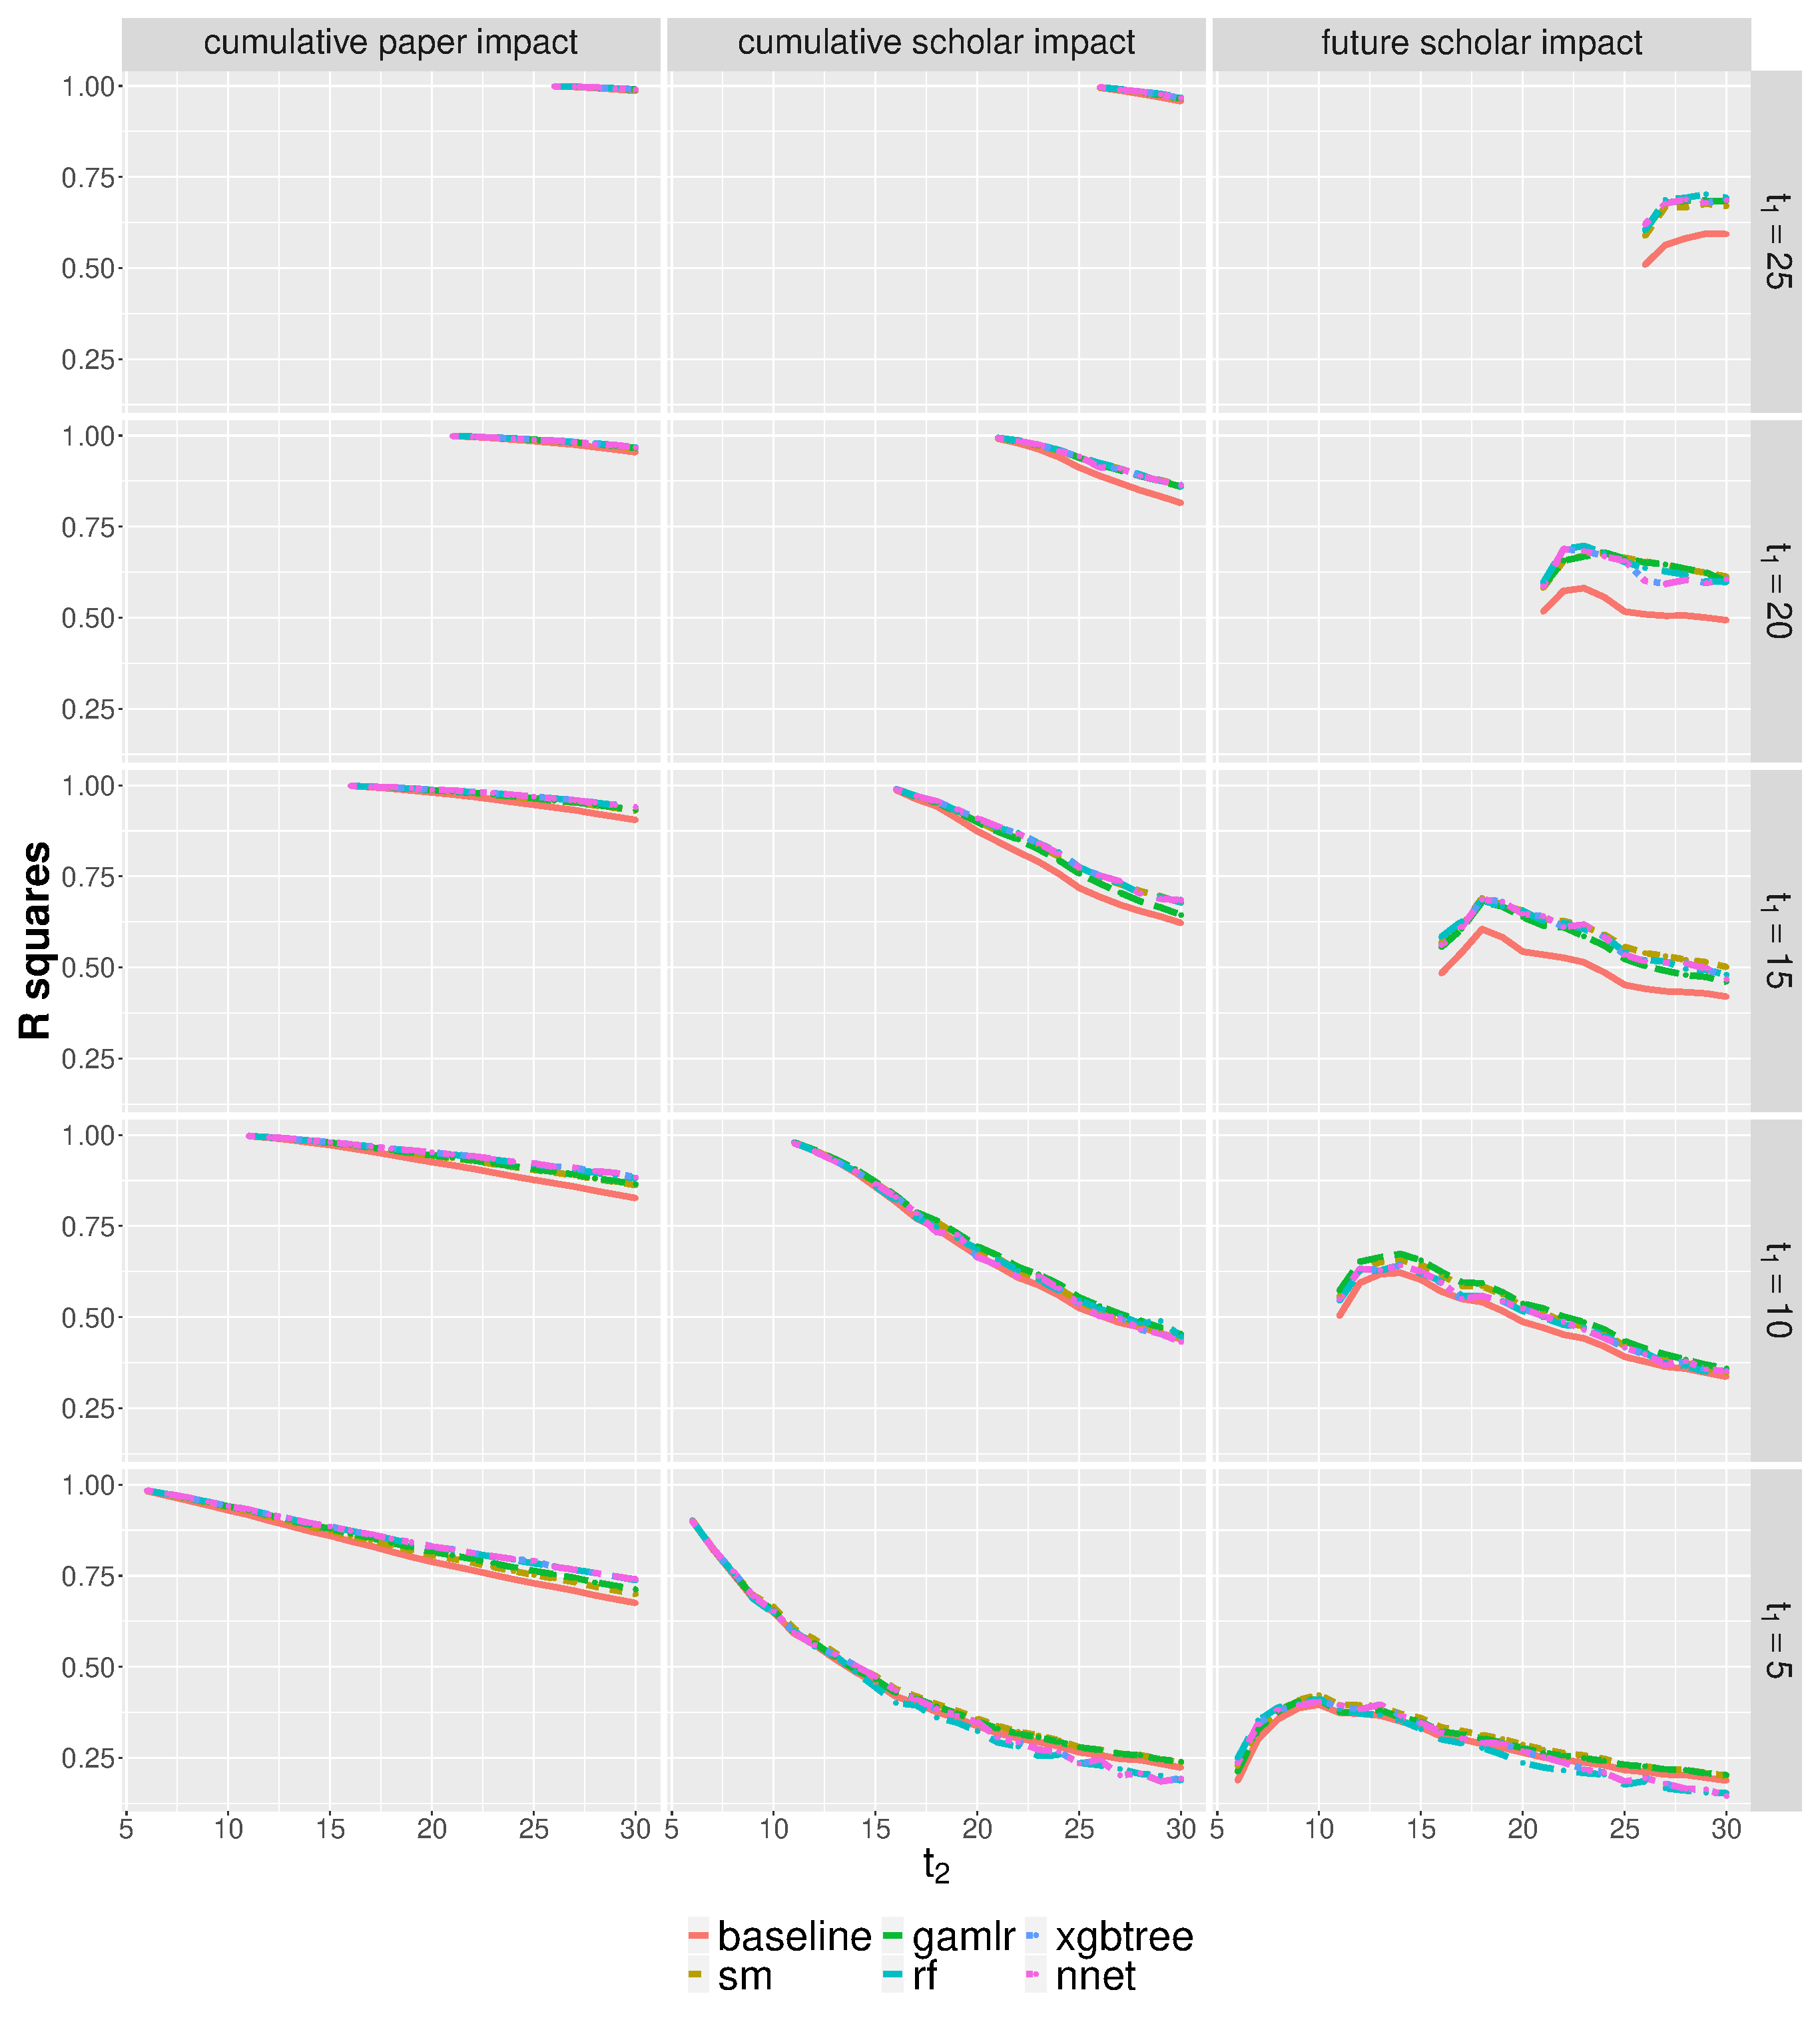
\includegraphics[width=\textwidth]{figures/pred_model/r2.eps}
    \caption[R squares of the predictive models]{Testing $R^2$ of the predictive models. The lasso, ridge, and elastic net are outperformed by the Gamma lasso and hence are ignored for a better visualization.}
    \label{fig:pred_r2}
\end{figure}







%\include{todo}
%\include{todiscuss}


\clearpage
%\bibliography{reference}
\printbibliography
%%!TEX root = main.tex
\clearpage
% fig:stableness_rp
% The rank percentile indicators are stable over publishing years 
\begin{figure}[ht!]
    \centering
    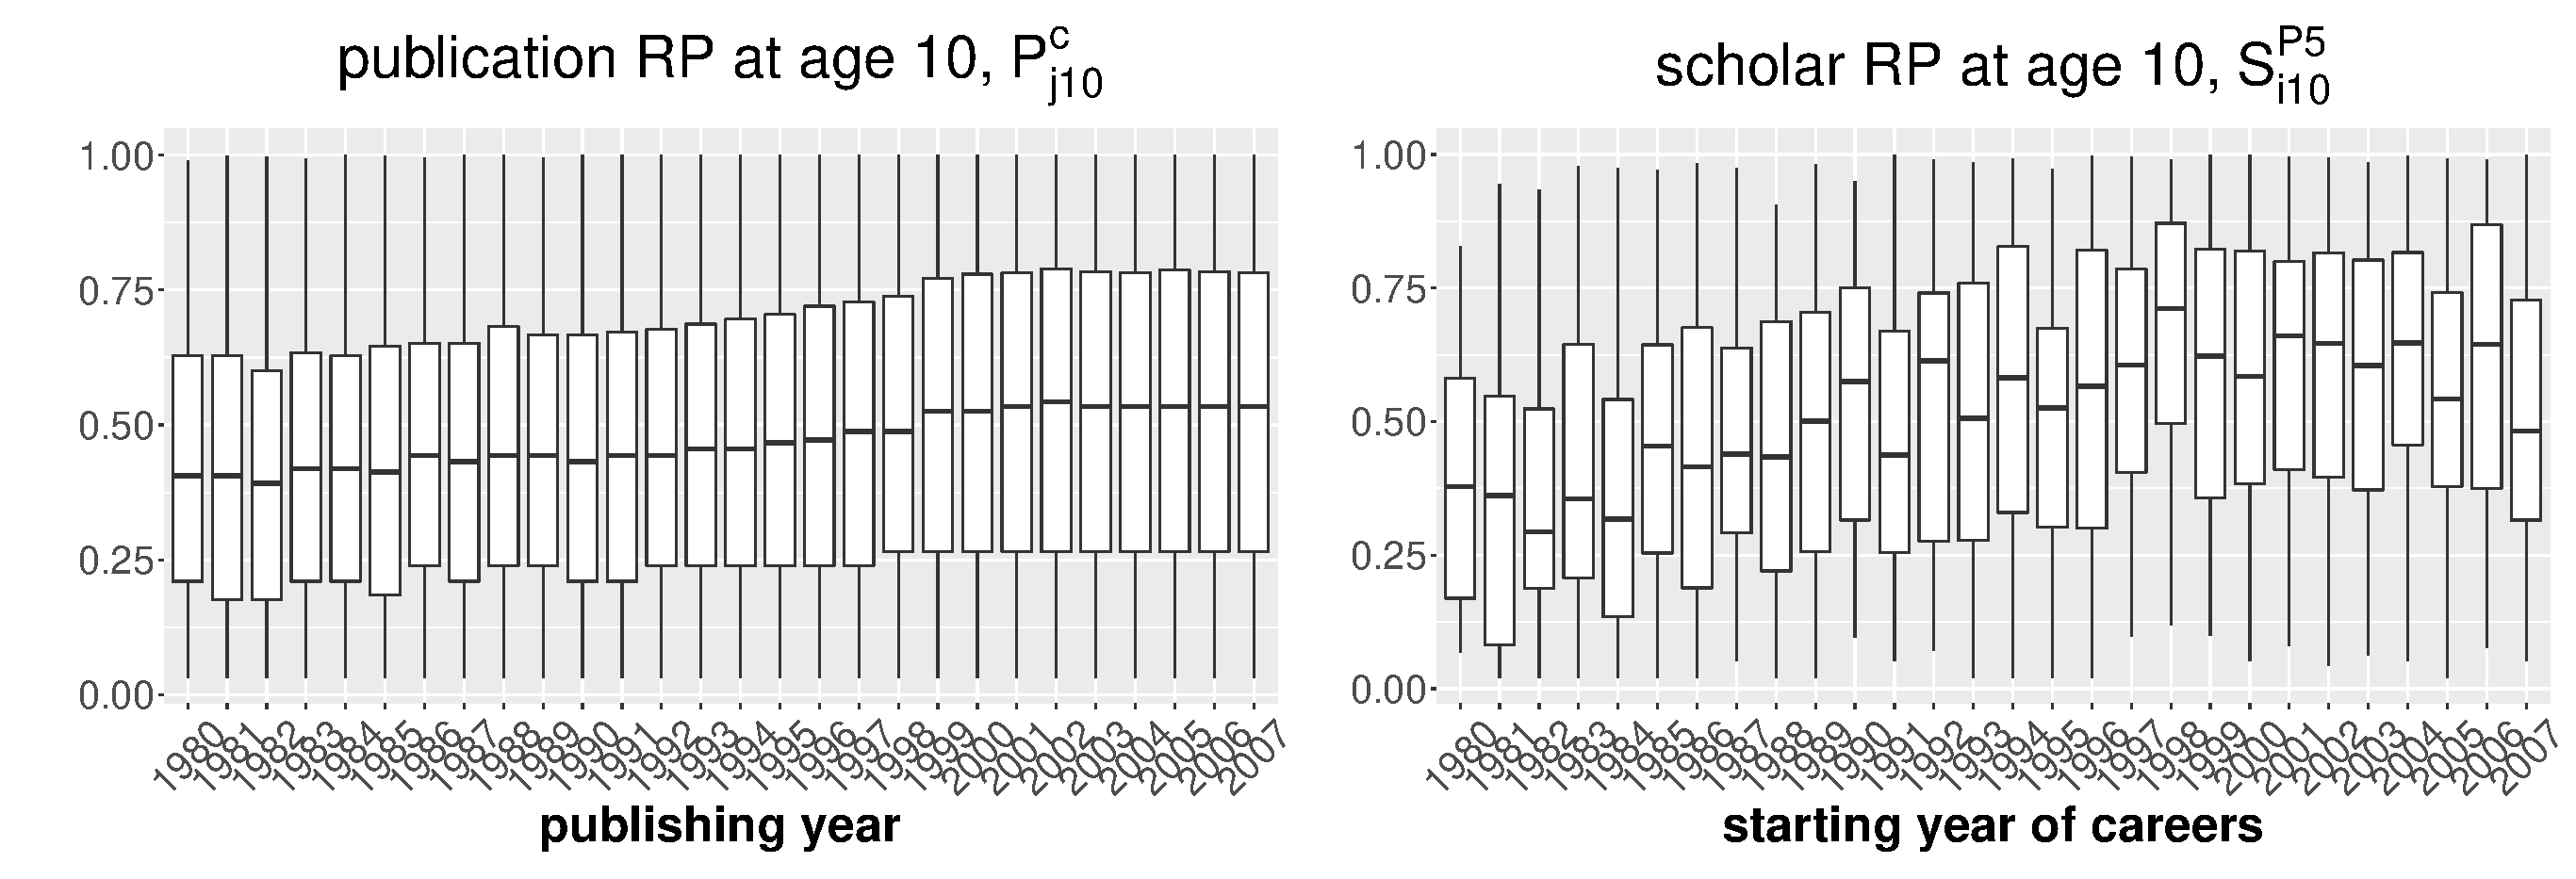
\includegraphics[width=\textwidth]{figures/exploratory/stationarity.eps}
    \caption{P$_{i10}^c$ grouped by the publication years and and S$_{i10}^{P5}$ grouped by the starting years of academic careers. The benchmark contains professors from various disciplines who receive their tenureships in year $2016$ or pubRP .}
    \label{fig:stableness_rp}
\end{figure}


% fig:panos
% show Panos as an example
\begin{figure}[ht!]
    \centering
    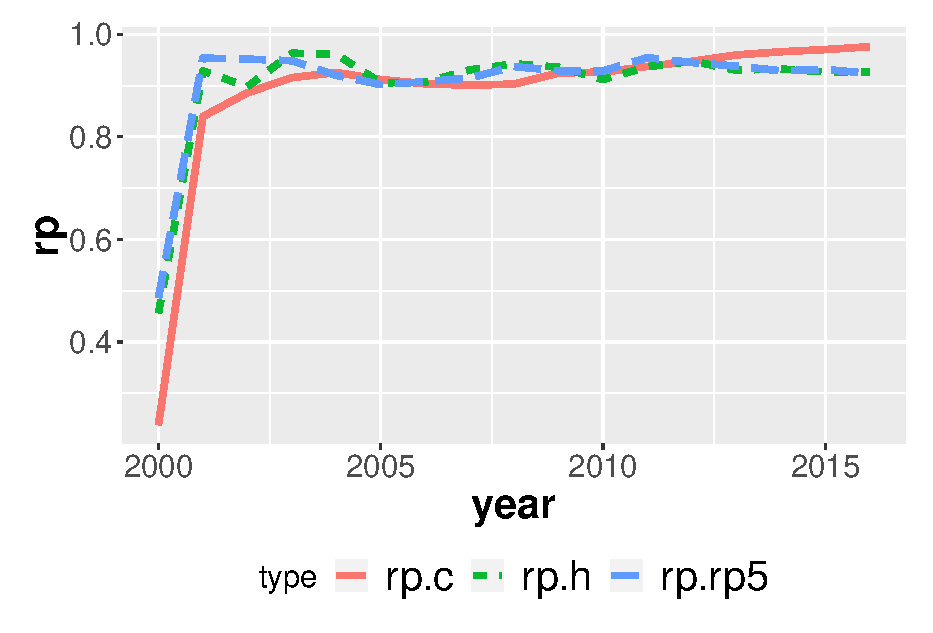
\includegraphics[width=0.7\textwidth]{figures/compare_autrp/panos.eps}
    \caption{The rank percentile indicators for Panos Ipeirotis. The benchmark contains all tenured professors by $2016$.}
    \label{fig:panos}
\end{figure}


% fig:simulated_authors
% show the difference between various author rp
\begin{figure}[ht!]
    \centering
    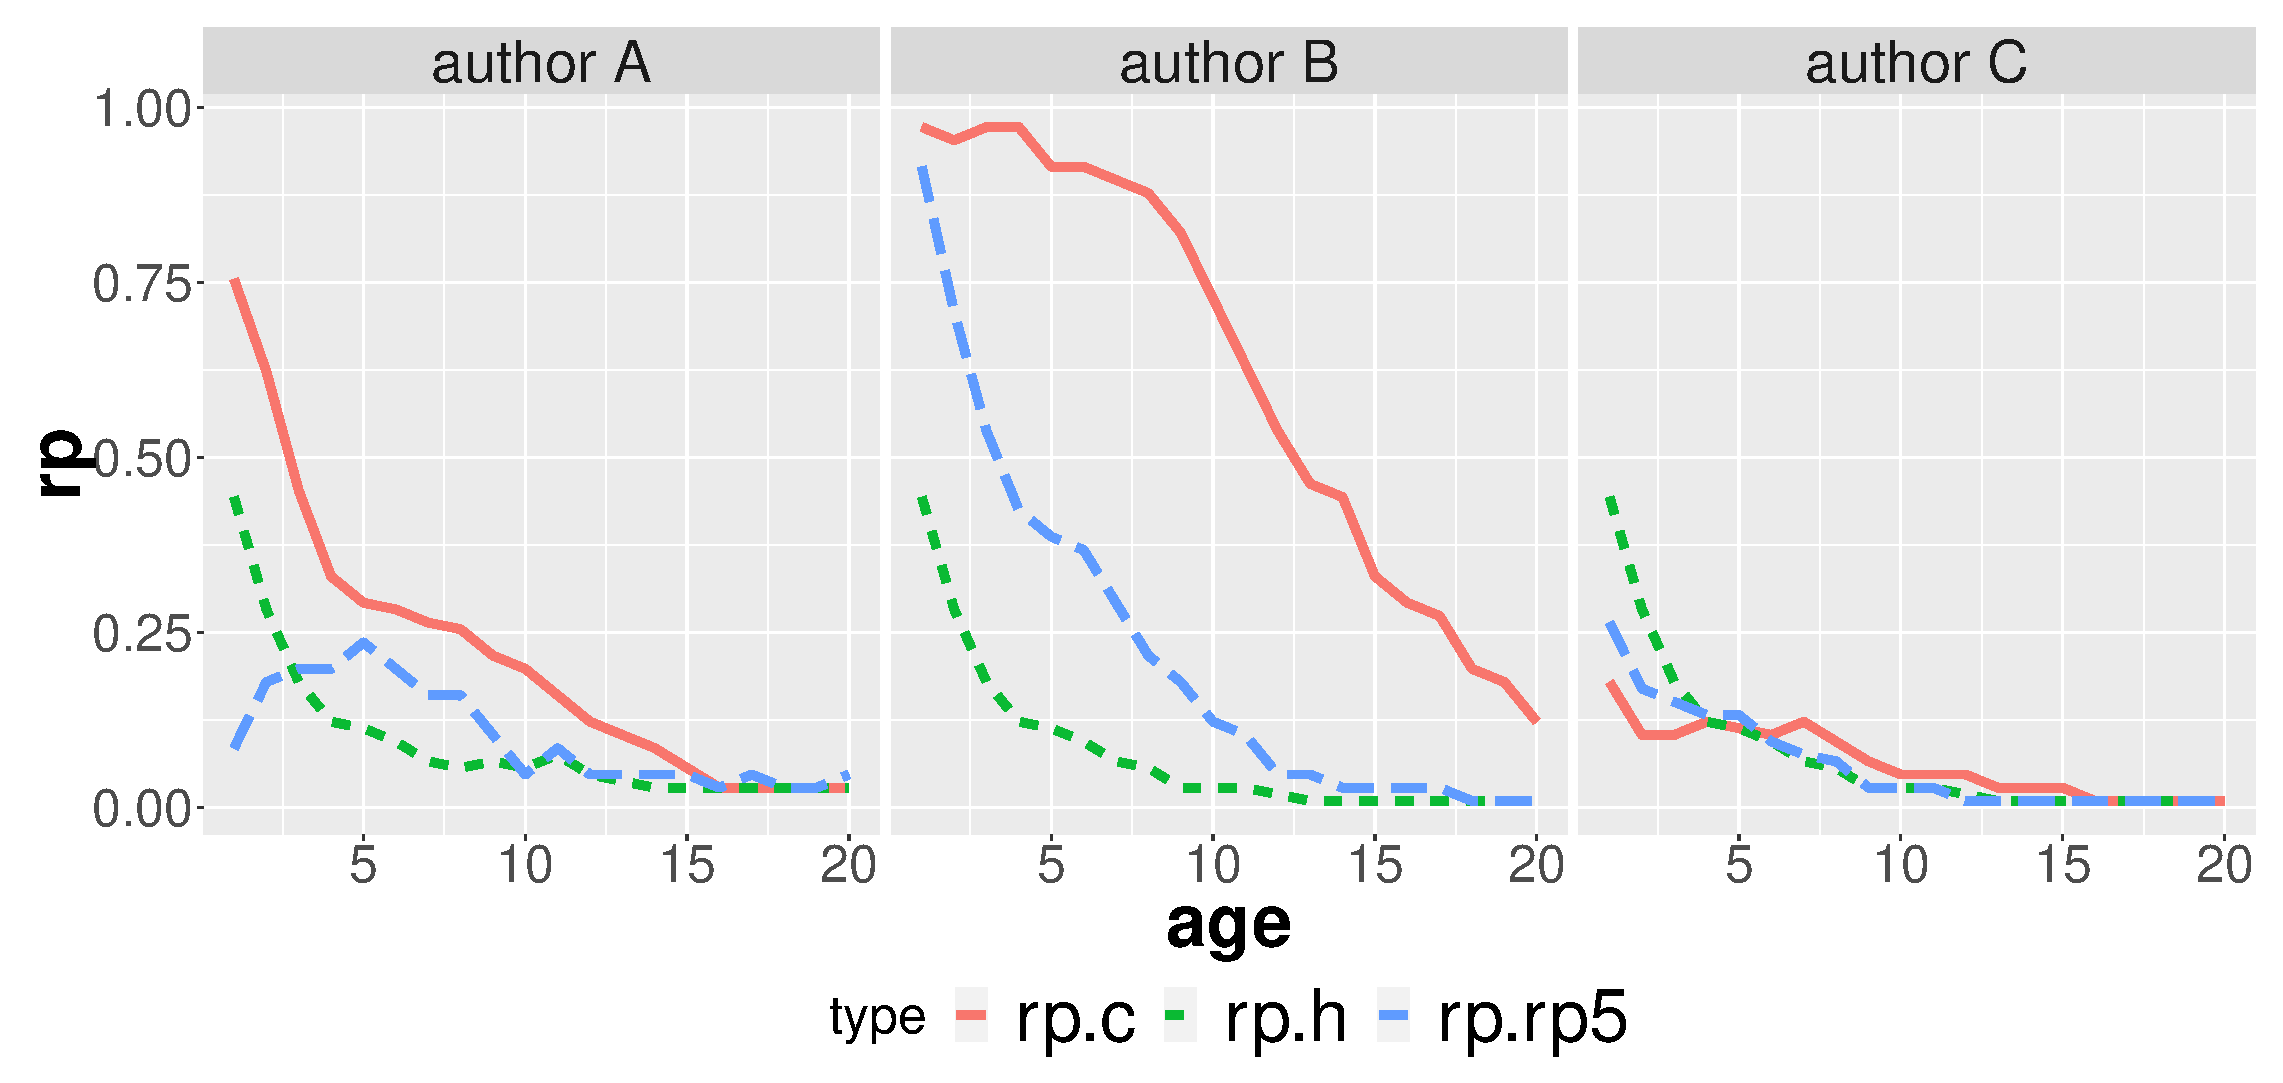
\includegraphics[width=\textwidth]{figures/compare_autrp/simulated_authors.eps}
    \caption{Three artificial authors to illustrate the difference between various types of author rank percentile indicators. Author A is highly productive at all ages but all of the works have little impact. Author B and author C only publish one paper at age $1$ throughout the entire careers, where the paper of author B has very high impact while the paper of author C has medium impact. The h-index of all authors at all ages are $1$. The benchmark contains authors in biology who start their careers from year $1990$.}
    \label{fig:simulated_authors}
\end{figure}


% fig:aut_rp_class
% class agreement among all the author rp
\begin{figure}[ht!]
    \centering
    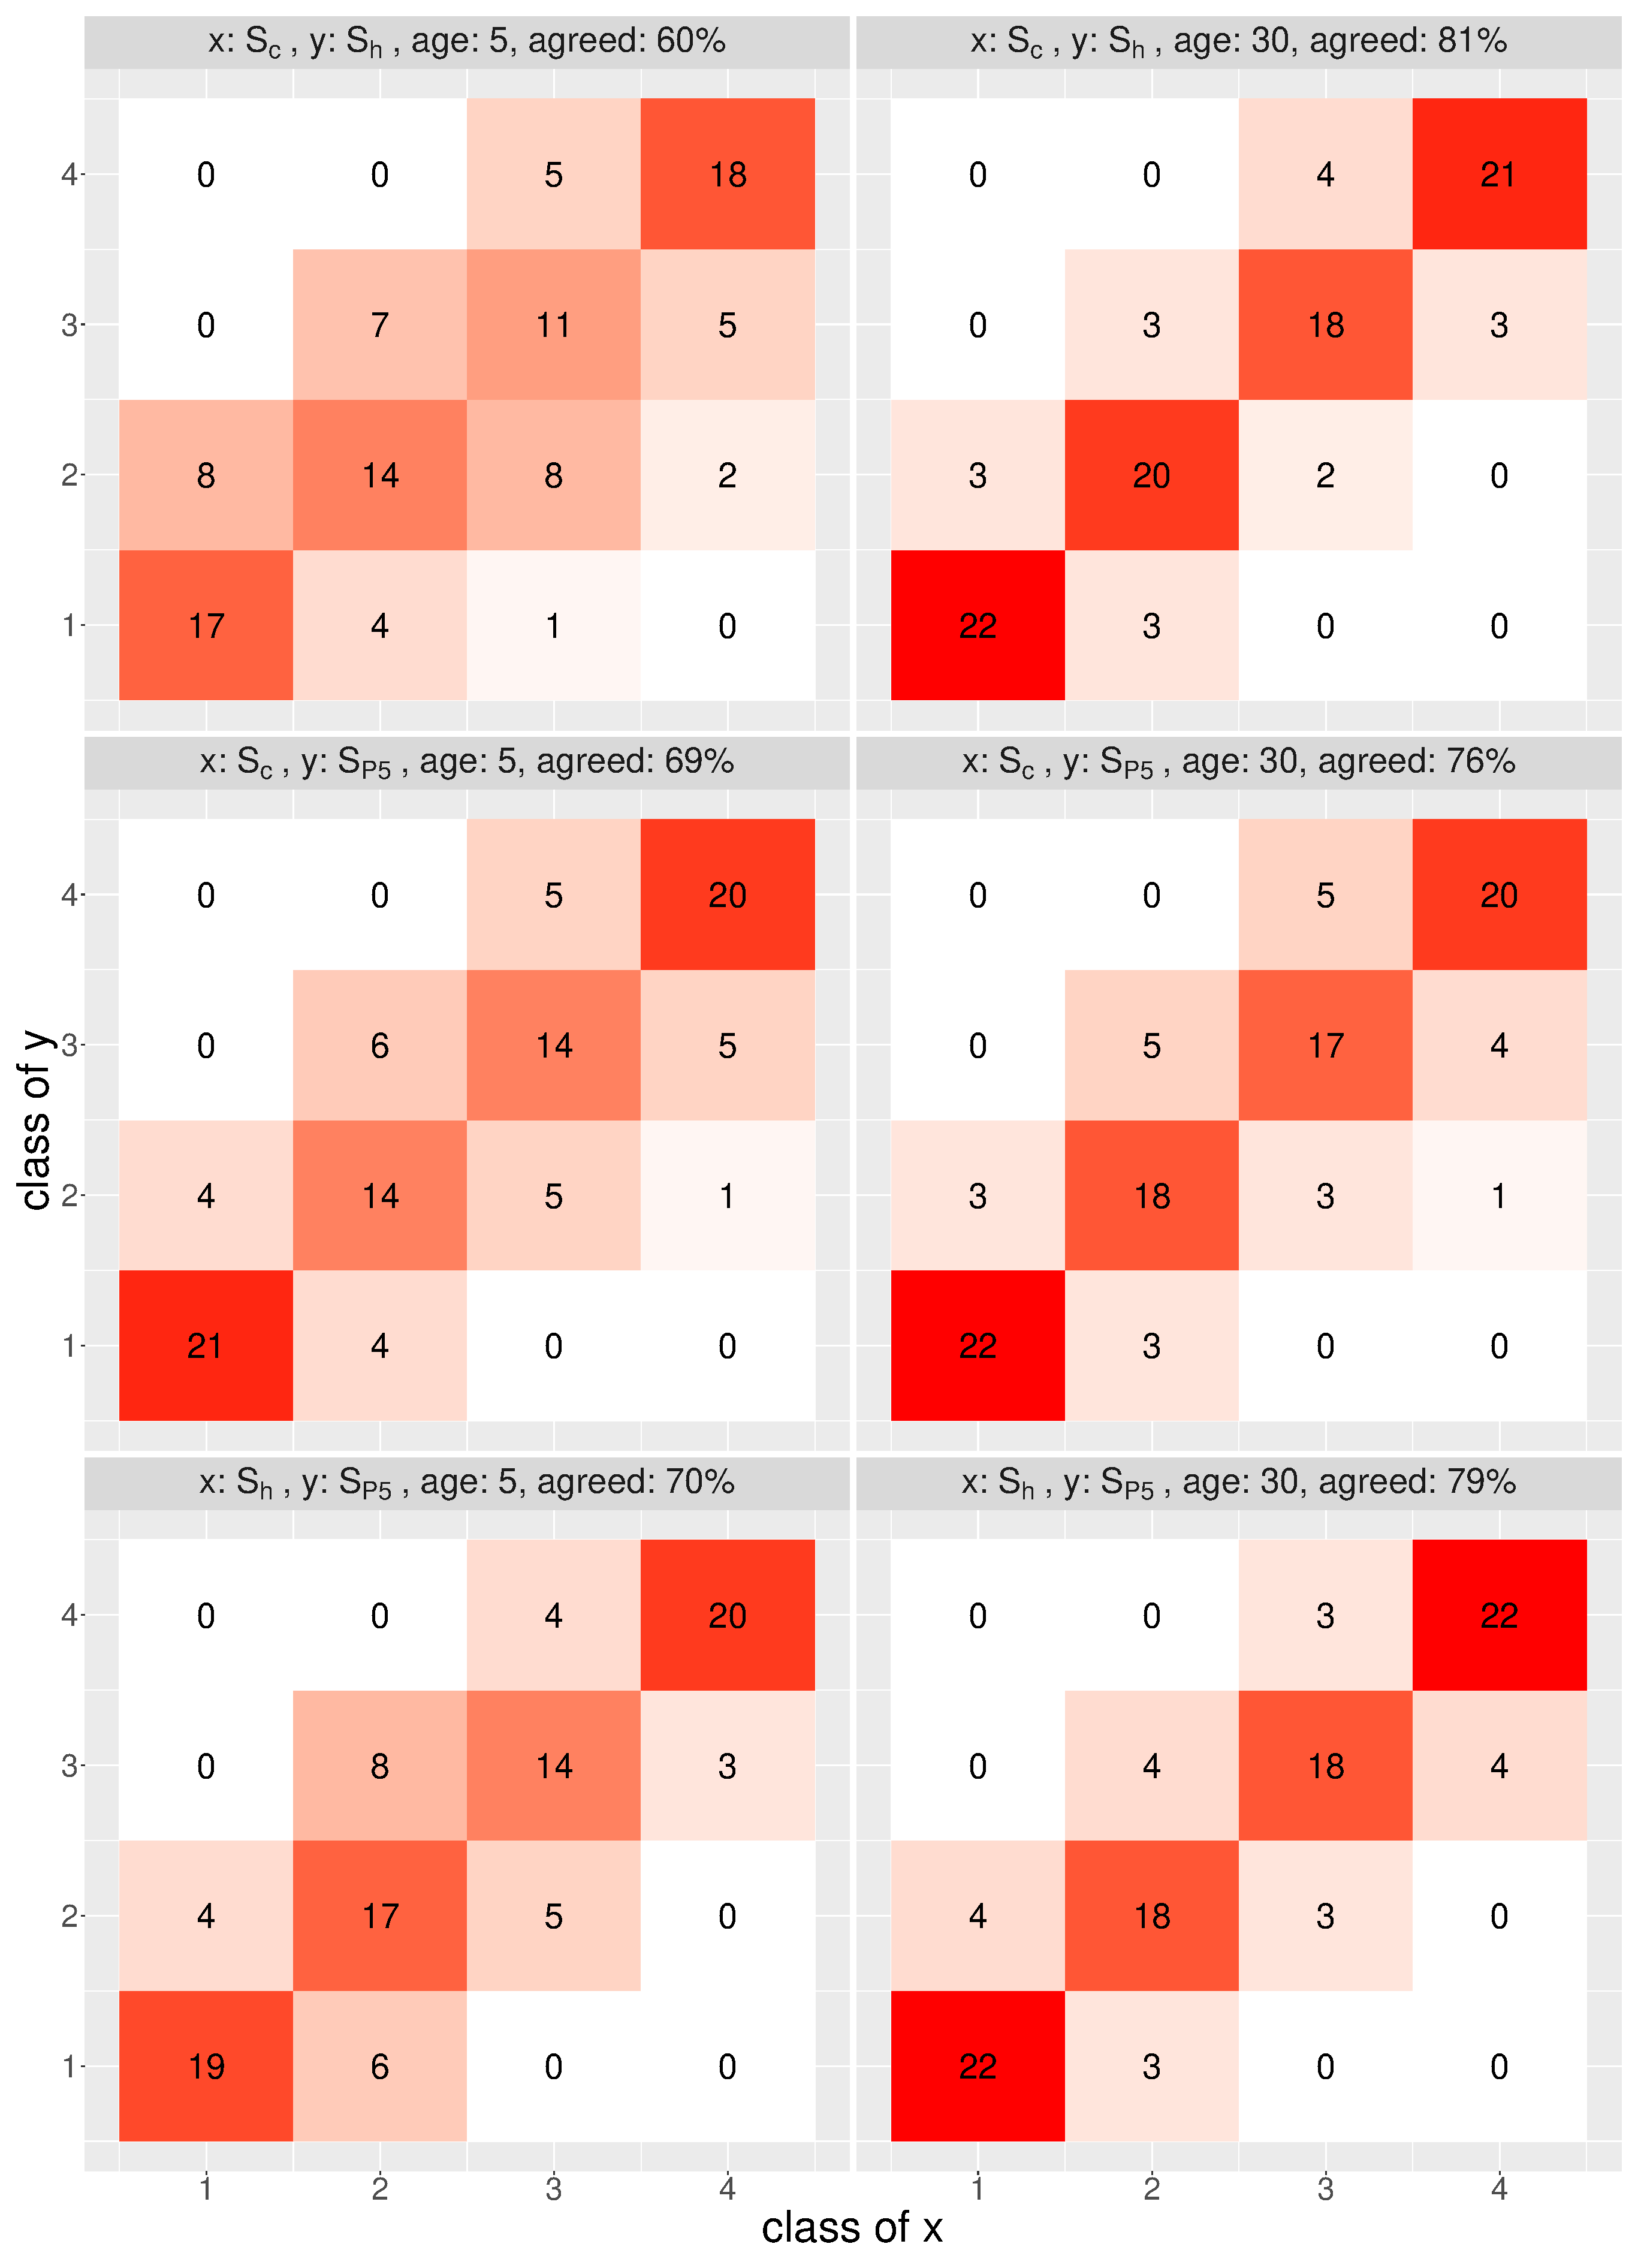
\includegraphics[width=0.88\textwidth]{figures/compare_autrp/heatmap_class_agreement.eps}
    \caption{Classifications of various types of author rp. Each rp is classified into four classes, class 1: $0 \le \text{rp} < 0.25$, class 2: $0.25 \le \text{rp} < 0.5$, class 3: $0.5 \le \text{rp} < 0.75$ and class 4: $0.75 \le \text{rp} \le 1$. The agreement of classifications (sum of the anti-diagonal elements) is displayed in the title of each panel. The benchmark is biology. The agreement for all three types is $51 \%$ at age $5$ and $68 \%$ at age $30$.}
    \label{fig:aut_rp_class}
\end{figure}

% publication rank percentile vs citations, predictability, Wang(2013)
\begin{figure}
     \centering
     \begin{subfigure}[b]{0.48\textwidth}
         \centering
         \includegraphics[width=\textwidth]{figures/pred_power/ncit_vs_pubrp/cit_age.pdf}
         \caption{}
         \label{fig:pred_cit_age}
     \end{subfigure}
     \hfill
     \begin{subfigure}[b]{0.48\textwidth}
         \centering
         \includegraphics[width=\textwidth]{figures/pred_power/ncit_vs_pubrp/rp_age.pdf}
         \caption{}
         \label{fig:pred_rp_age}
     \end{subfigure}
     \hfill
     \begin{subfigure}[b]{0.48\textwidth}
         \centering
         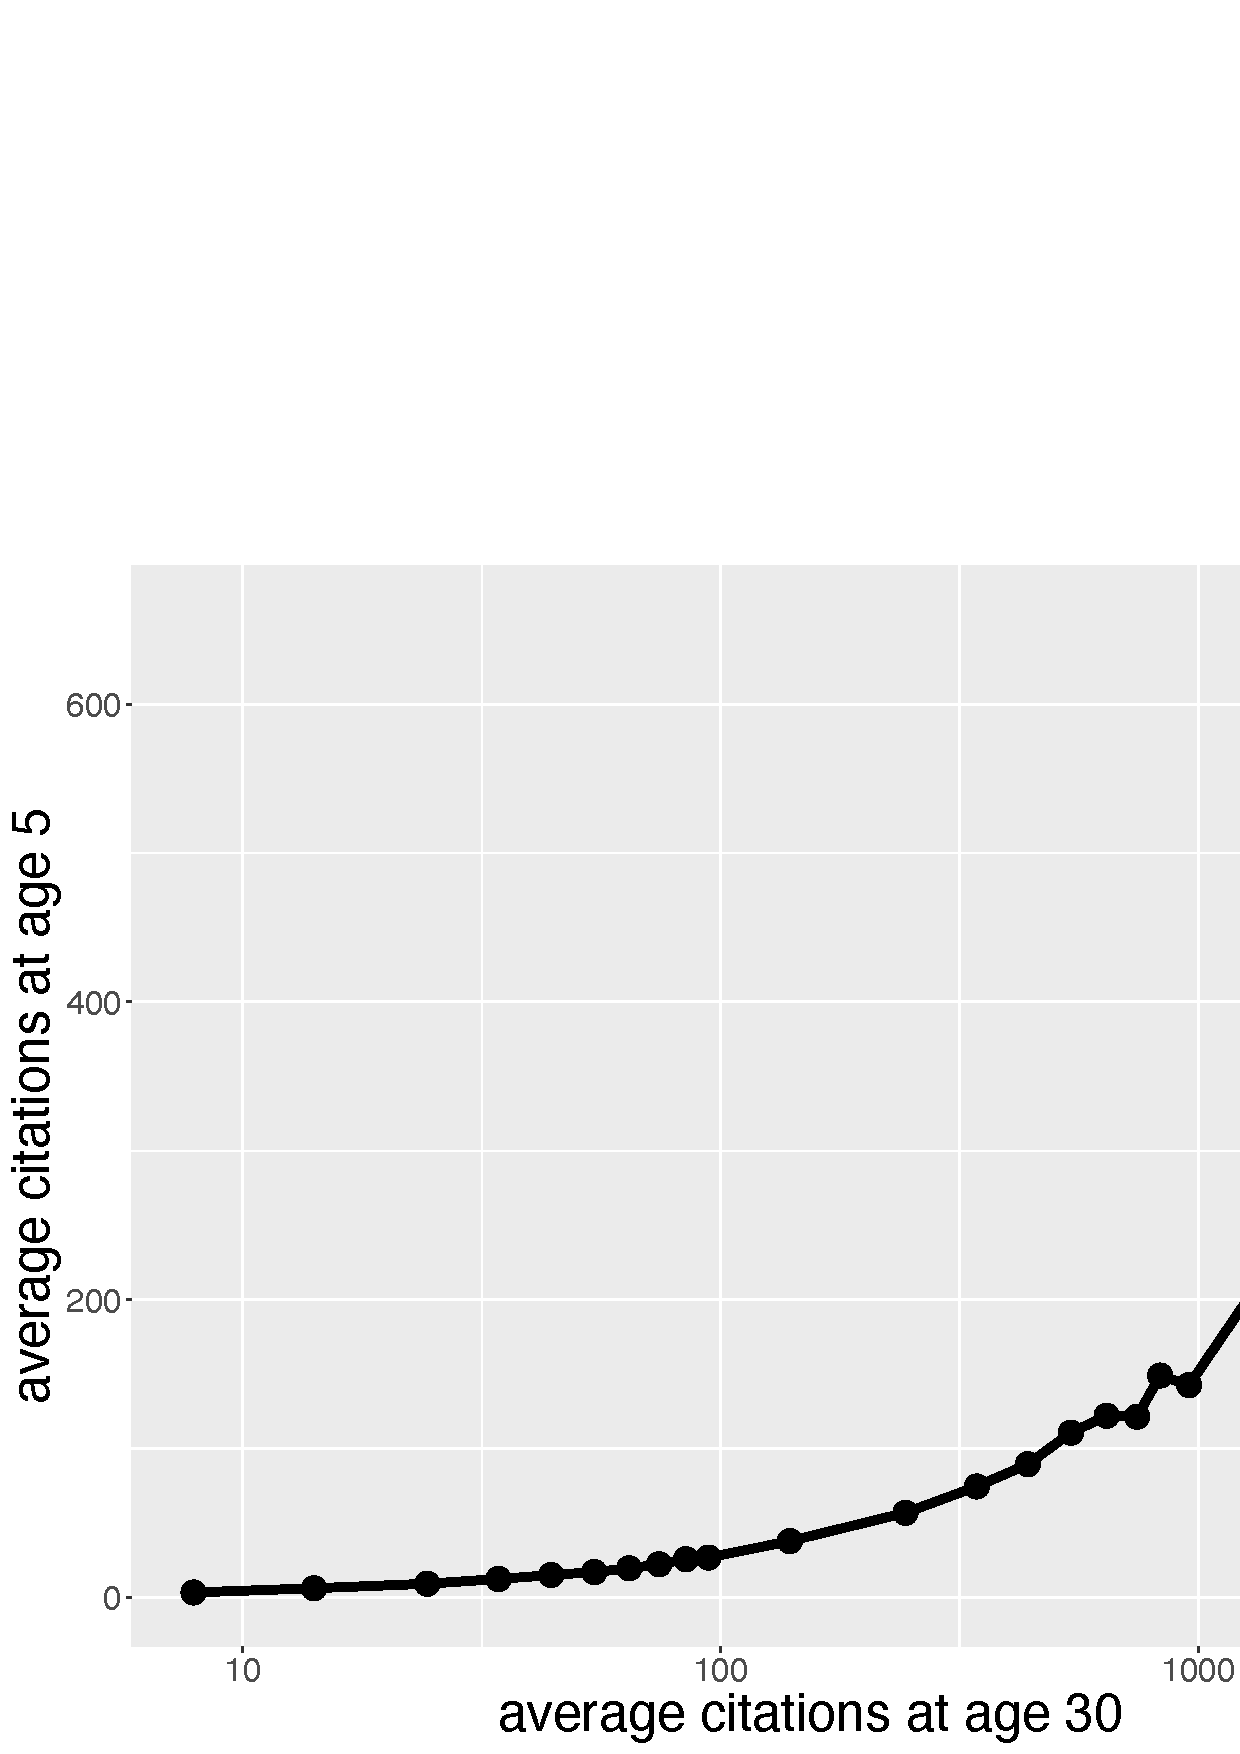
\includegraphics[width=\textwidth]{figures/pred_power/ncit_vs_pubrp/cit_cit.pdf}
         \caption{}
         \label{fig:pred_cit_cit}
     \end{subfigure}
     \hfill
     \begin{subfigure}[b]{0.48\textwidth}
         \centering
         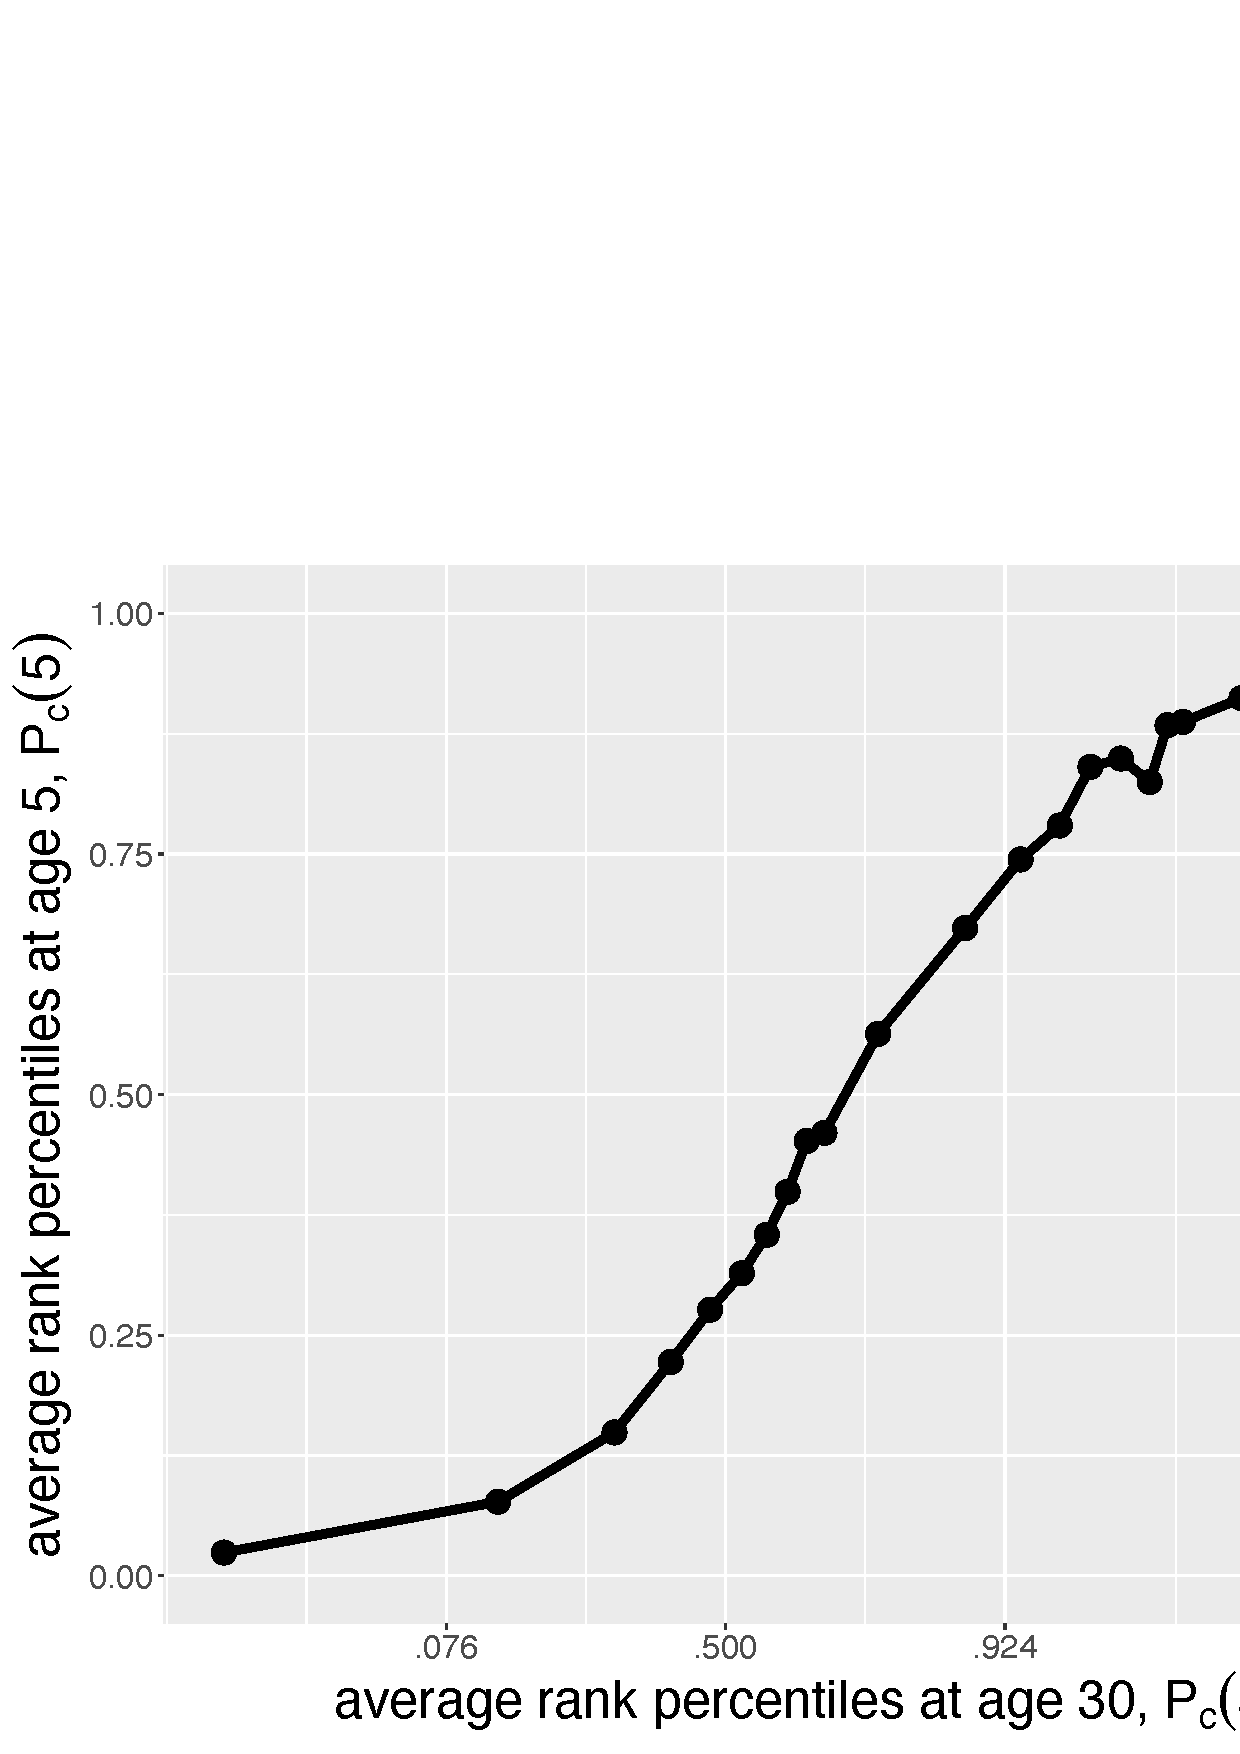
\includegraphics[width=\textwidth]{figures/pred_power/ncit_vs_pubrp/rp_rp.pdf}
         \caption{}
         \label{fig:pred_rp_rp}
     \end{subfigure}
        \caption{The predictability of citations and rank percentiles. The benchmark here is biology. Figure \ref{fig:pred_cit_age} and \ref{fig:pred_rp_age} show the cumulative citations and the corresponding rank percentiles for papers that have $50$ citations by age $5$. Figure \ref{fig:pred_cit_cit} displays the average citations by age $5$ over the average citations by age $30$, for sets of publications, which are pre-specified by dividing the range of $\overline{c_{j 30}}$ into equal intervals in the log scale. Figure \ref{fig:pred_rp_rp} shows the corresponding average rank percentiles for the same sets of publications. Note that we do not claim originality for these plots, as figures \ref{fig:pred_cit_age} and \ref{fig:pred_cit_cit} have been illustrated via a different dataset\supercite{Wang2013}.}
        \label{fig:pub_cit_rp_pred}
\end{figure}


% publication rank percentile, heat map of correlations
\begin{figure}[ht!]
    \centering
    \begin{subfigure}[b]{0.8\textwidth}
        \centering
             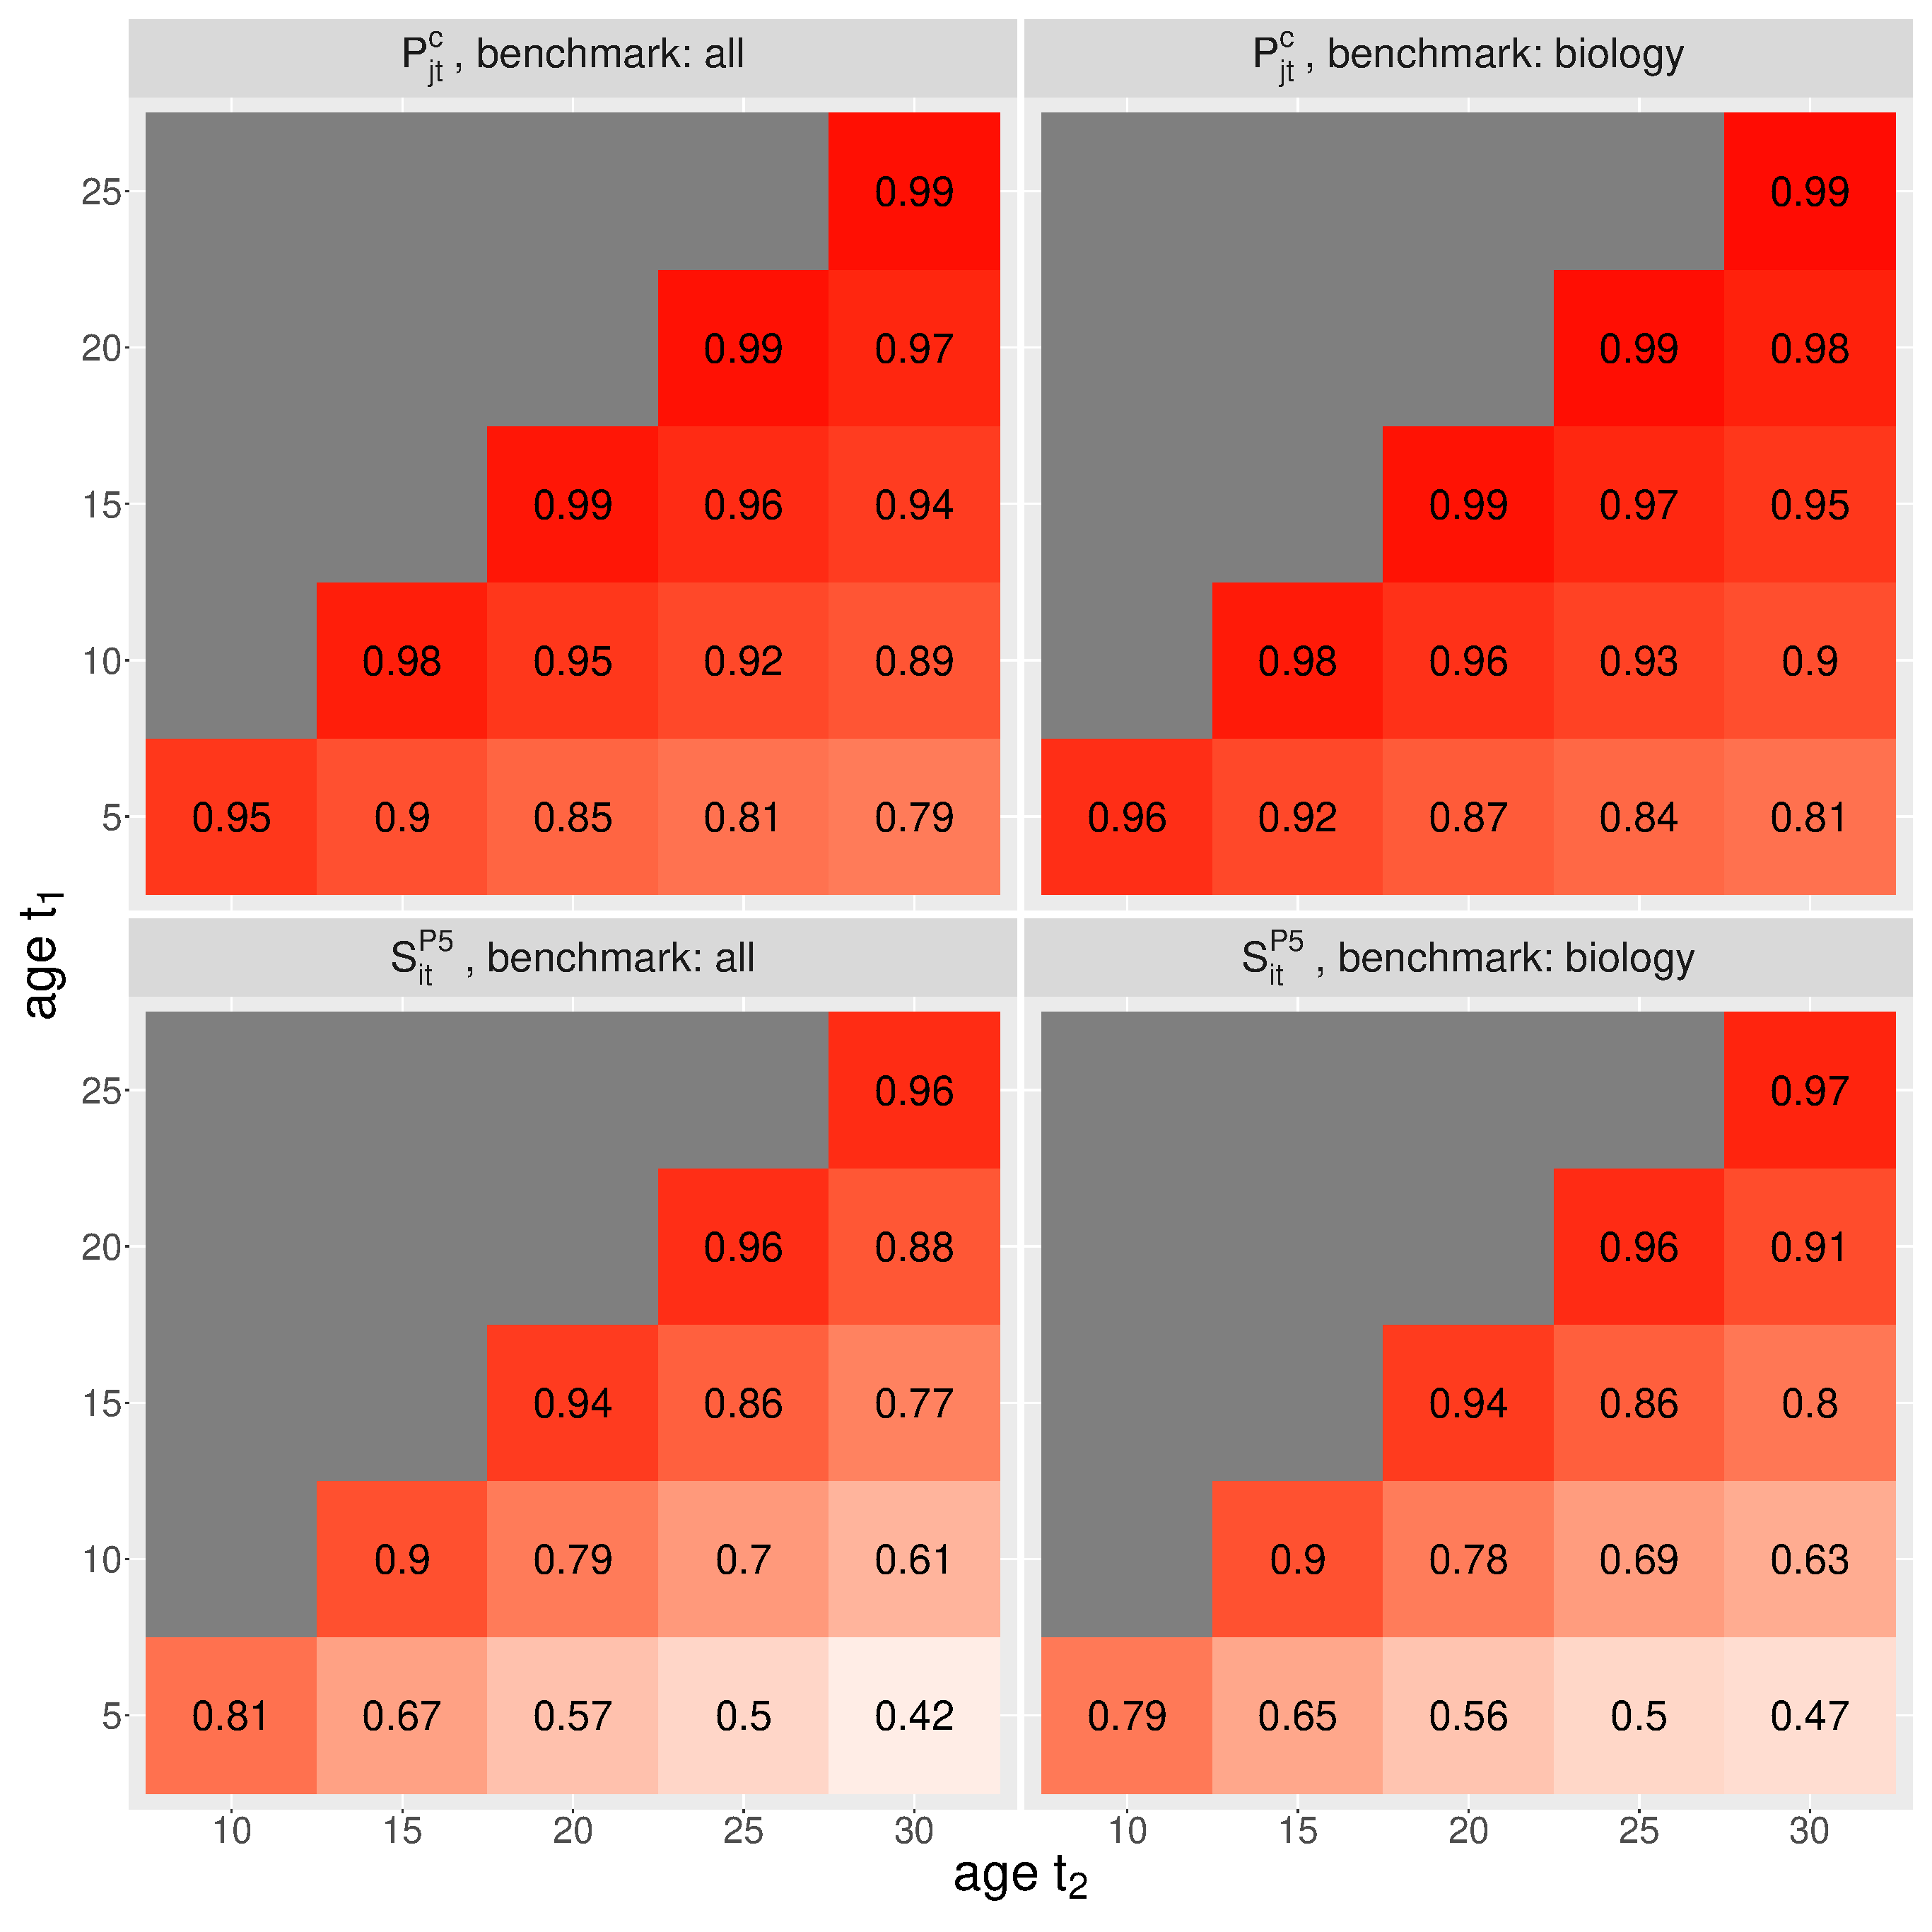
\includegraphics[width=\textwidth]{figures/pred_power/current/heatmap_cor.eps}
         \caption{Predict the cumulative impacts}
         \label{fig:hm_rp_current}
    \end{subfigure}
    
    \begin{subfigure}[b]{0.8\textwidth}
        \centering
             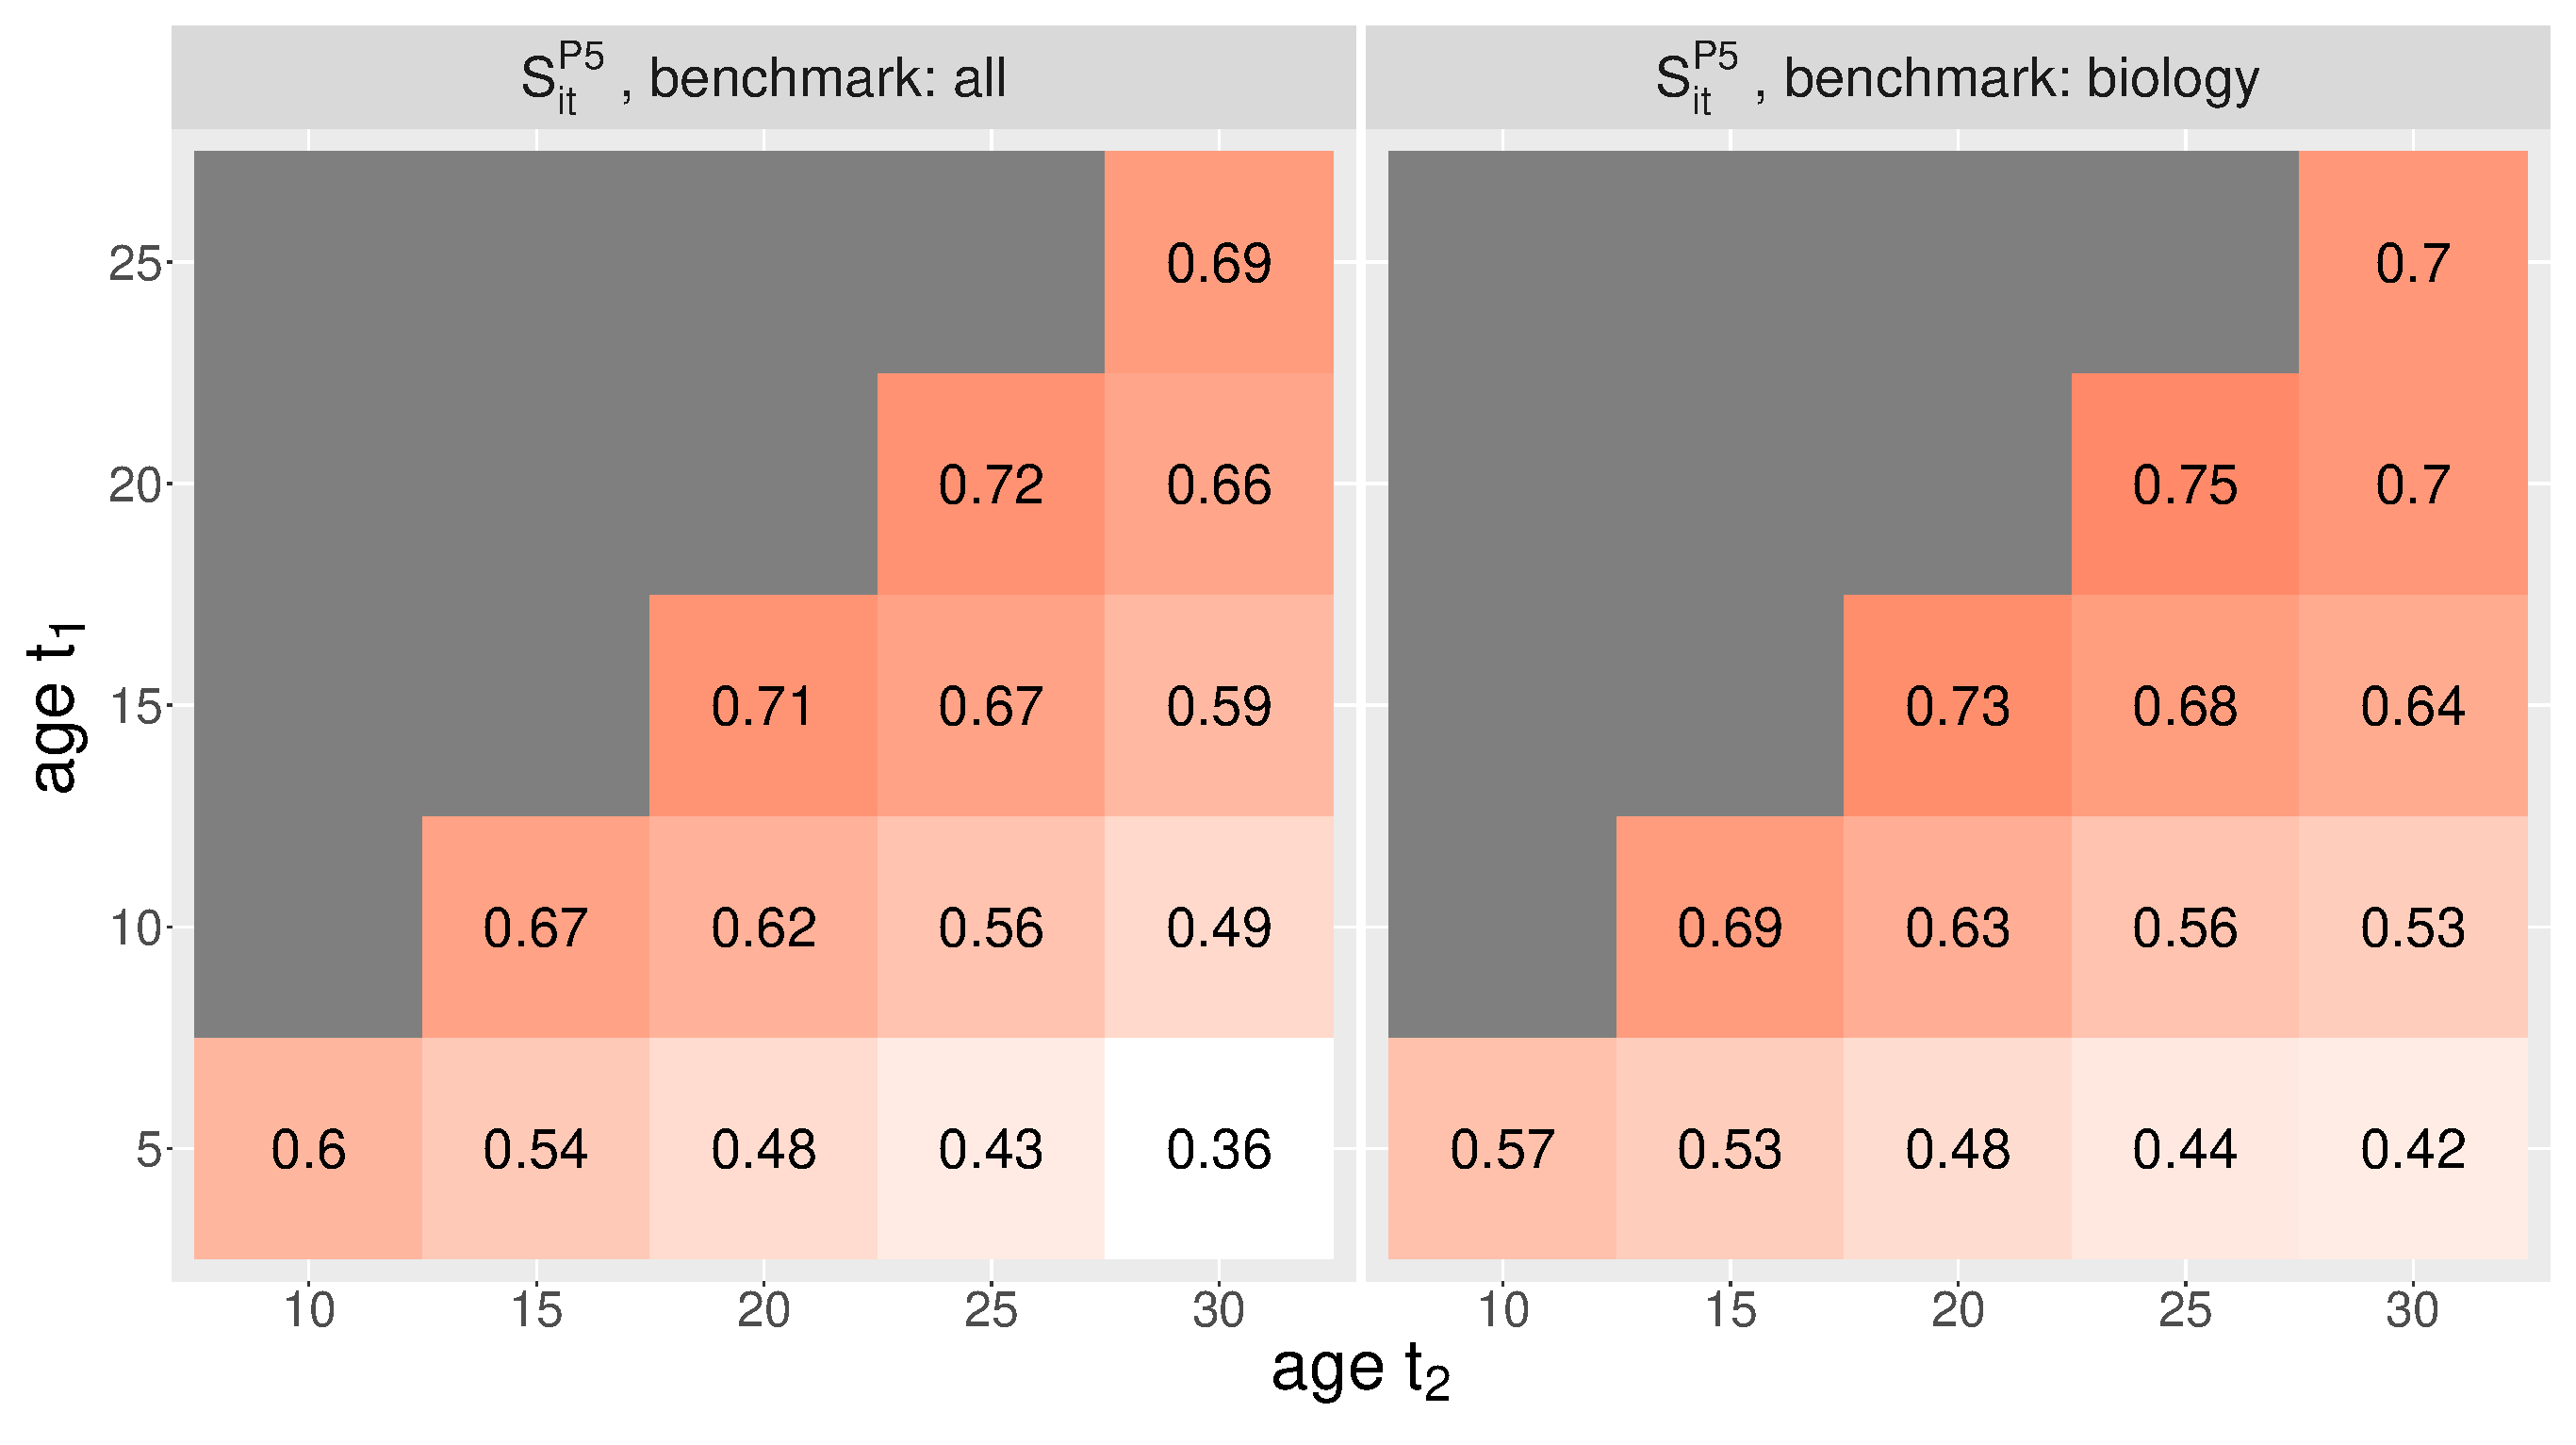
\includegraphics[width=\textwidth]{figures/pred_power/future/heatmap_cor.eps}
         \caption{Predict the future scientific output}
         \label{fig:hm_rp_future}
    \end{subfigure}
    \caption{The Pearson's correlation between rp indicators at two different ages. }
    \label{fig:hm_rp}
\end{figure}
\begin{figure}[ht!]
    \centering
    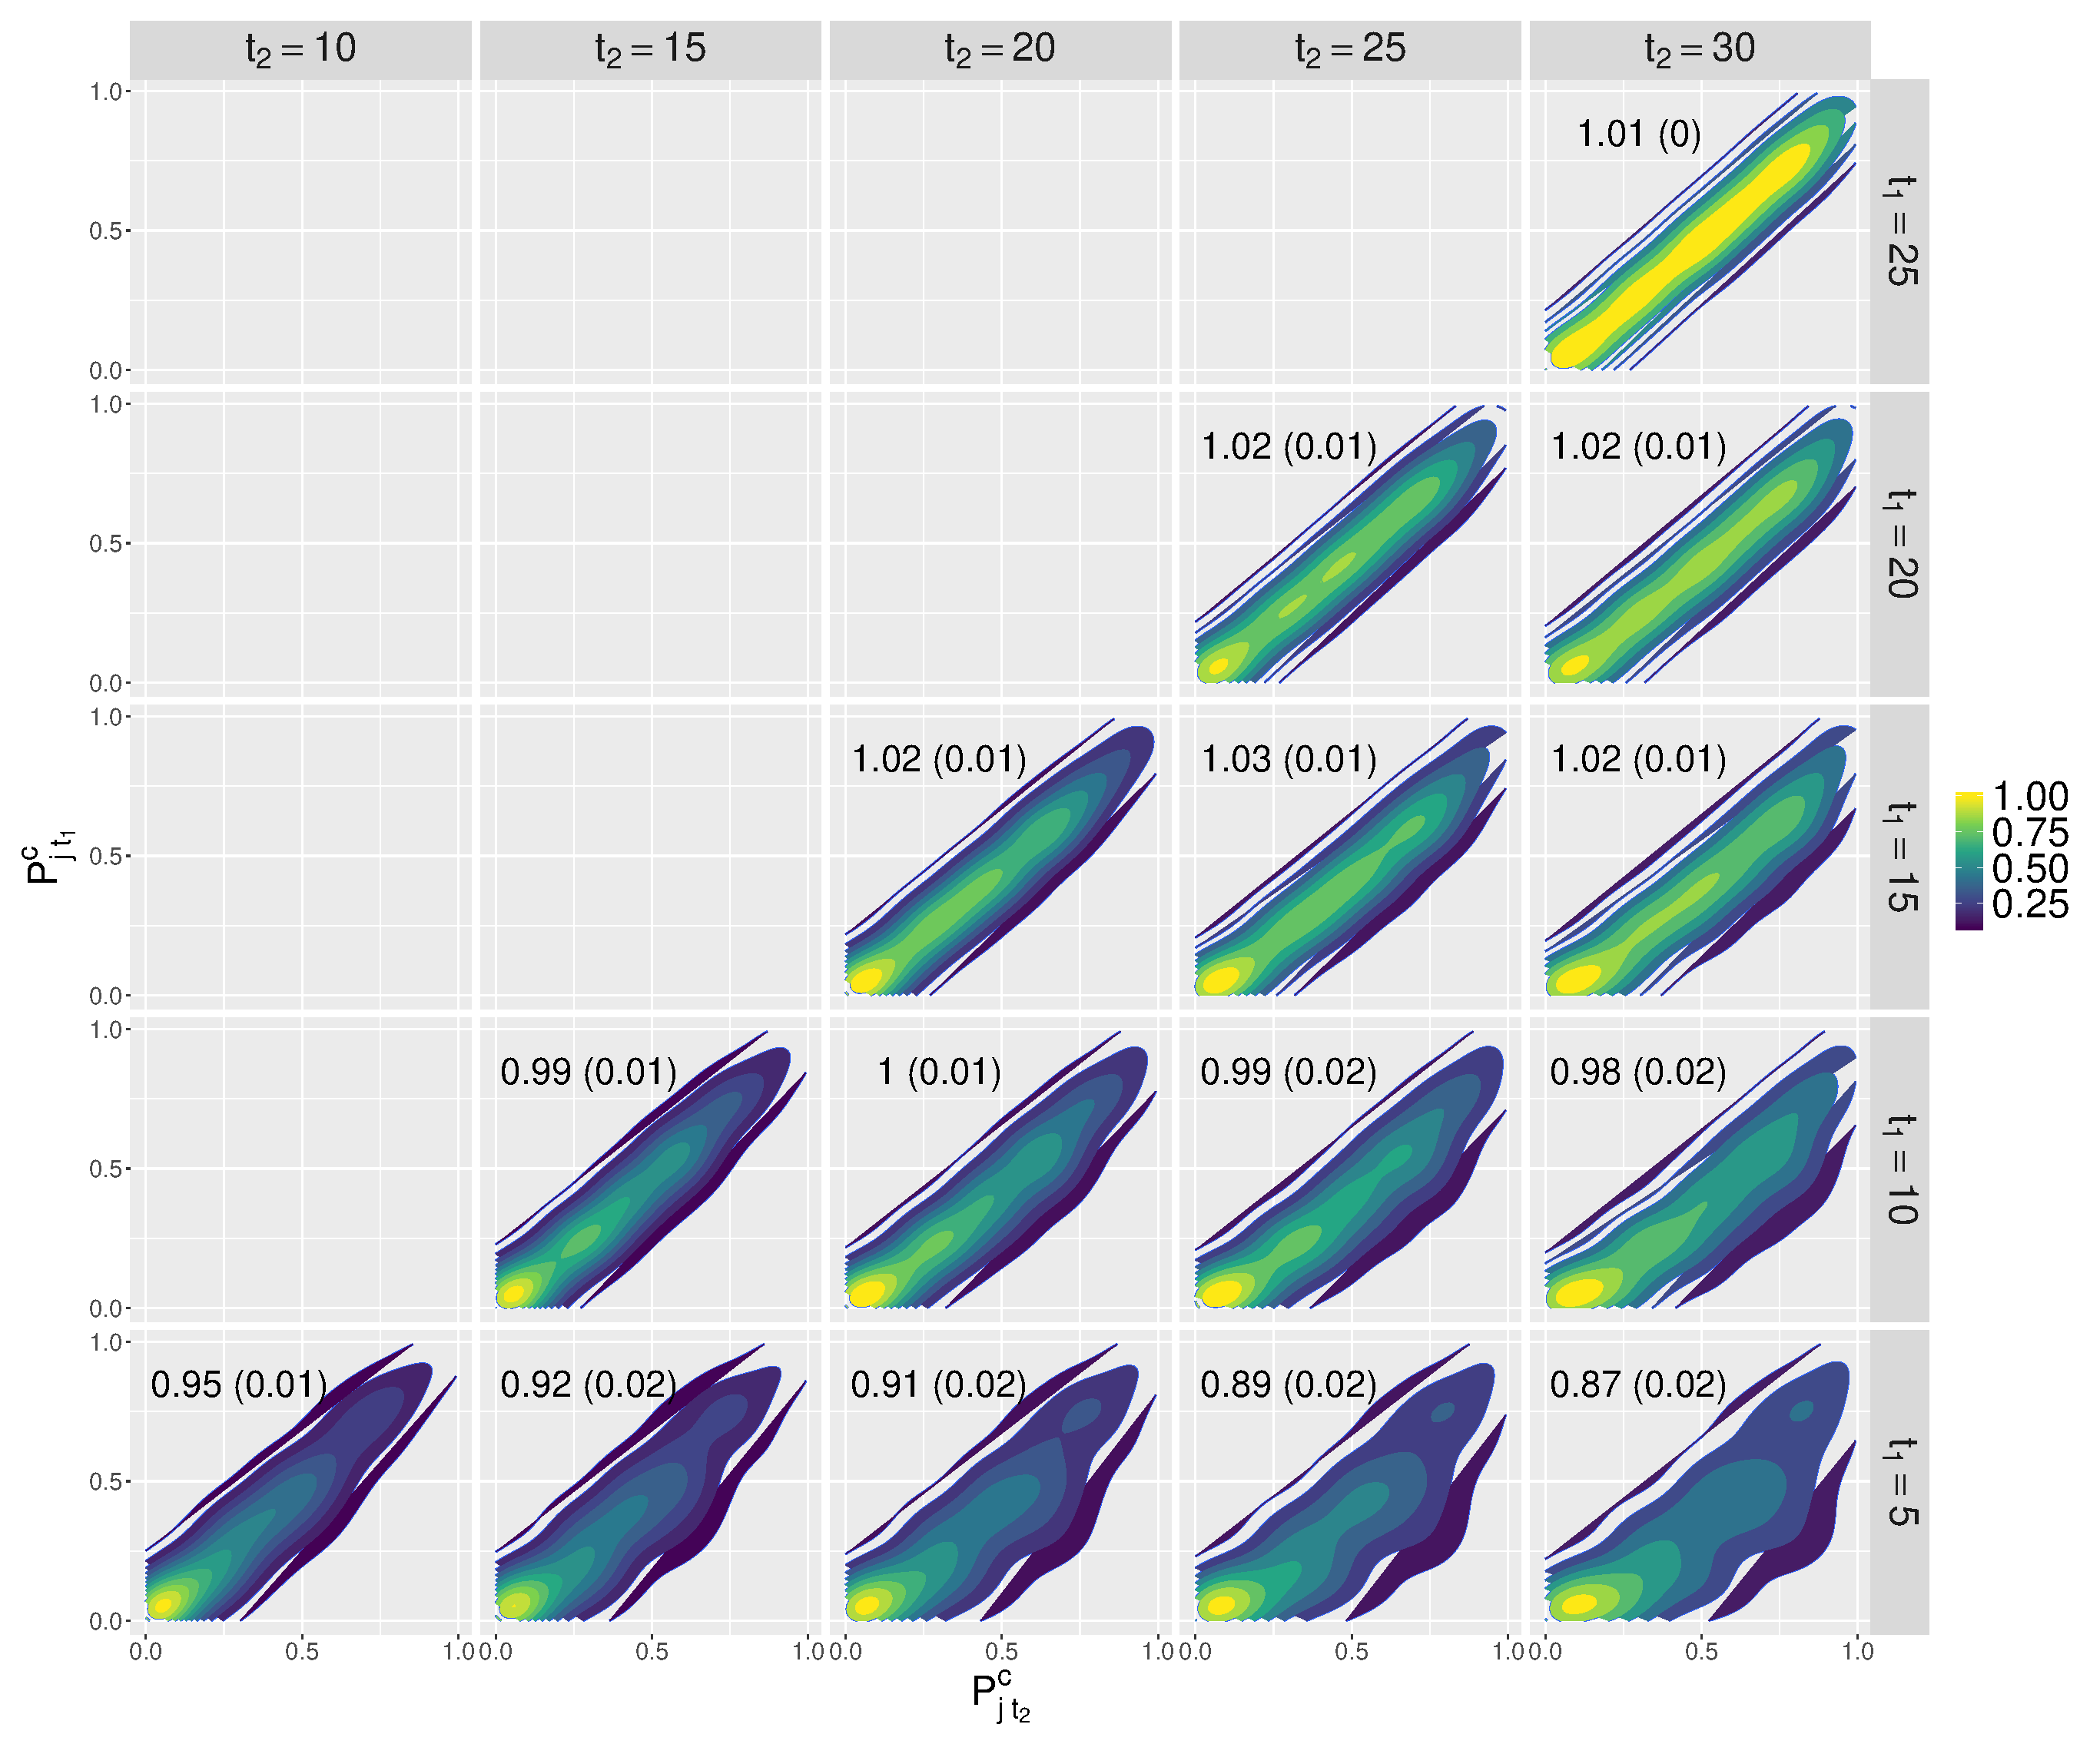
\includegraphics[width=\textwidth]{figures/pred_power/pubrp/scatter_bio1980.eps}
    \caption{Kernel density estimation of the scatters of rp.c$_{\cdot \tau_1}$ and rp.c$_{\cdot \tau_2}$. Meanwhile, we fit a simple linear regression of rp.c$_{\cdot \tau_2}$ upon rp.c$_{\cdot \tau_1}$. The estimated coefficient of rp.c$_{\cdot \tau_1}$ and the corresponding standard error (in the bracket) are displayed in each facet. The benchmark here includes all publications in biology and written in $1980$.}
    \label{fig:scatter_pubrp_bio1980}
\end{figure}

\iffalse
% author rank percentile, heat map of correlations
\begin{figure}[ht!]
    \centering
    \includegraphics[width=\textwidth]{figures/pred_power/autrp/heatmap_cor_all.eps}
    \caption{The Pearson's correlation between rp at two different ages, for various types of author rp. The benchmark includes all the authors.}
    \label{fig:hm_autrp_all}
\end{figure}
\begin{figure}[ht!]
    \centering
    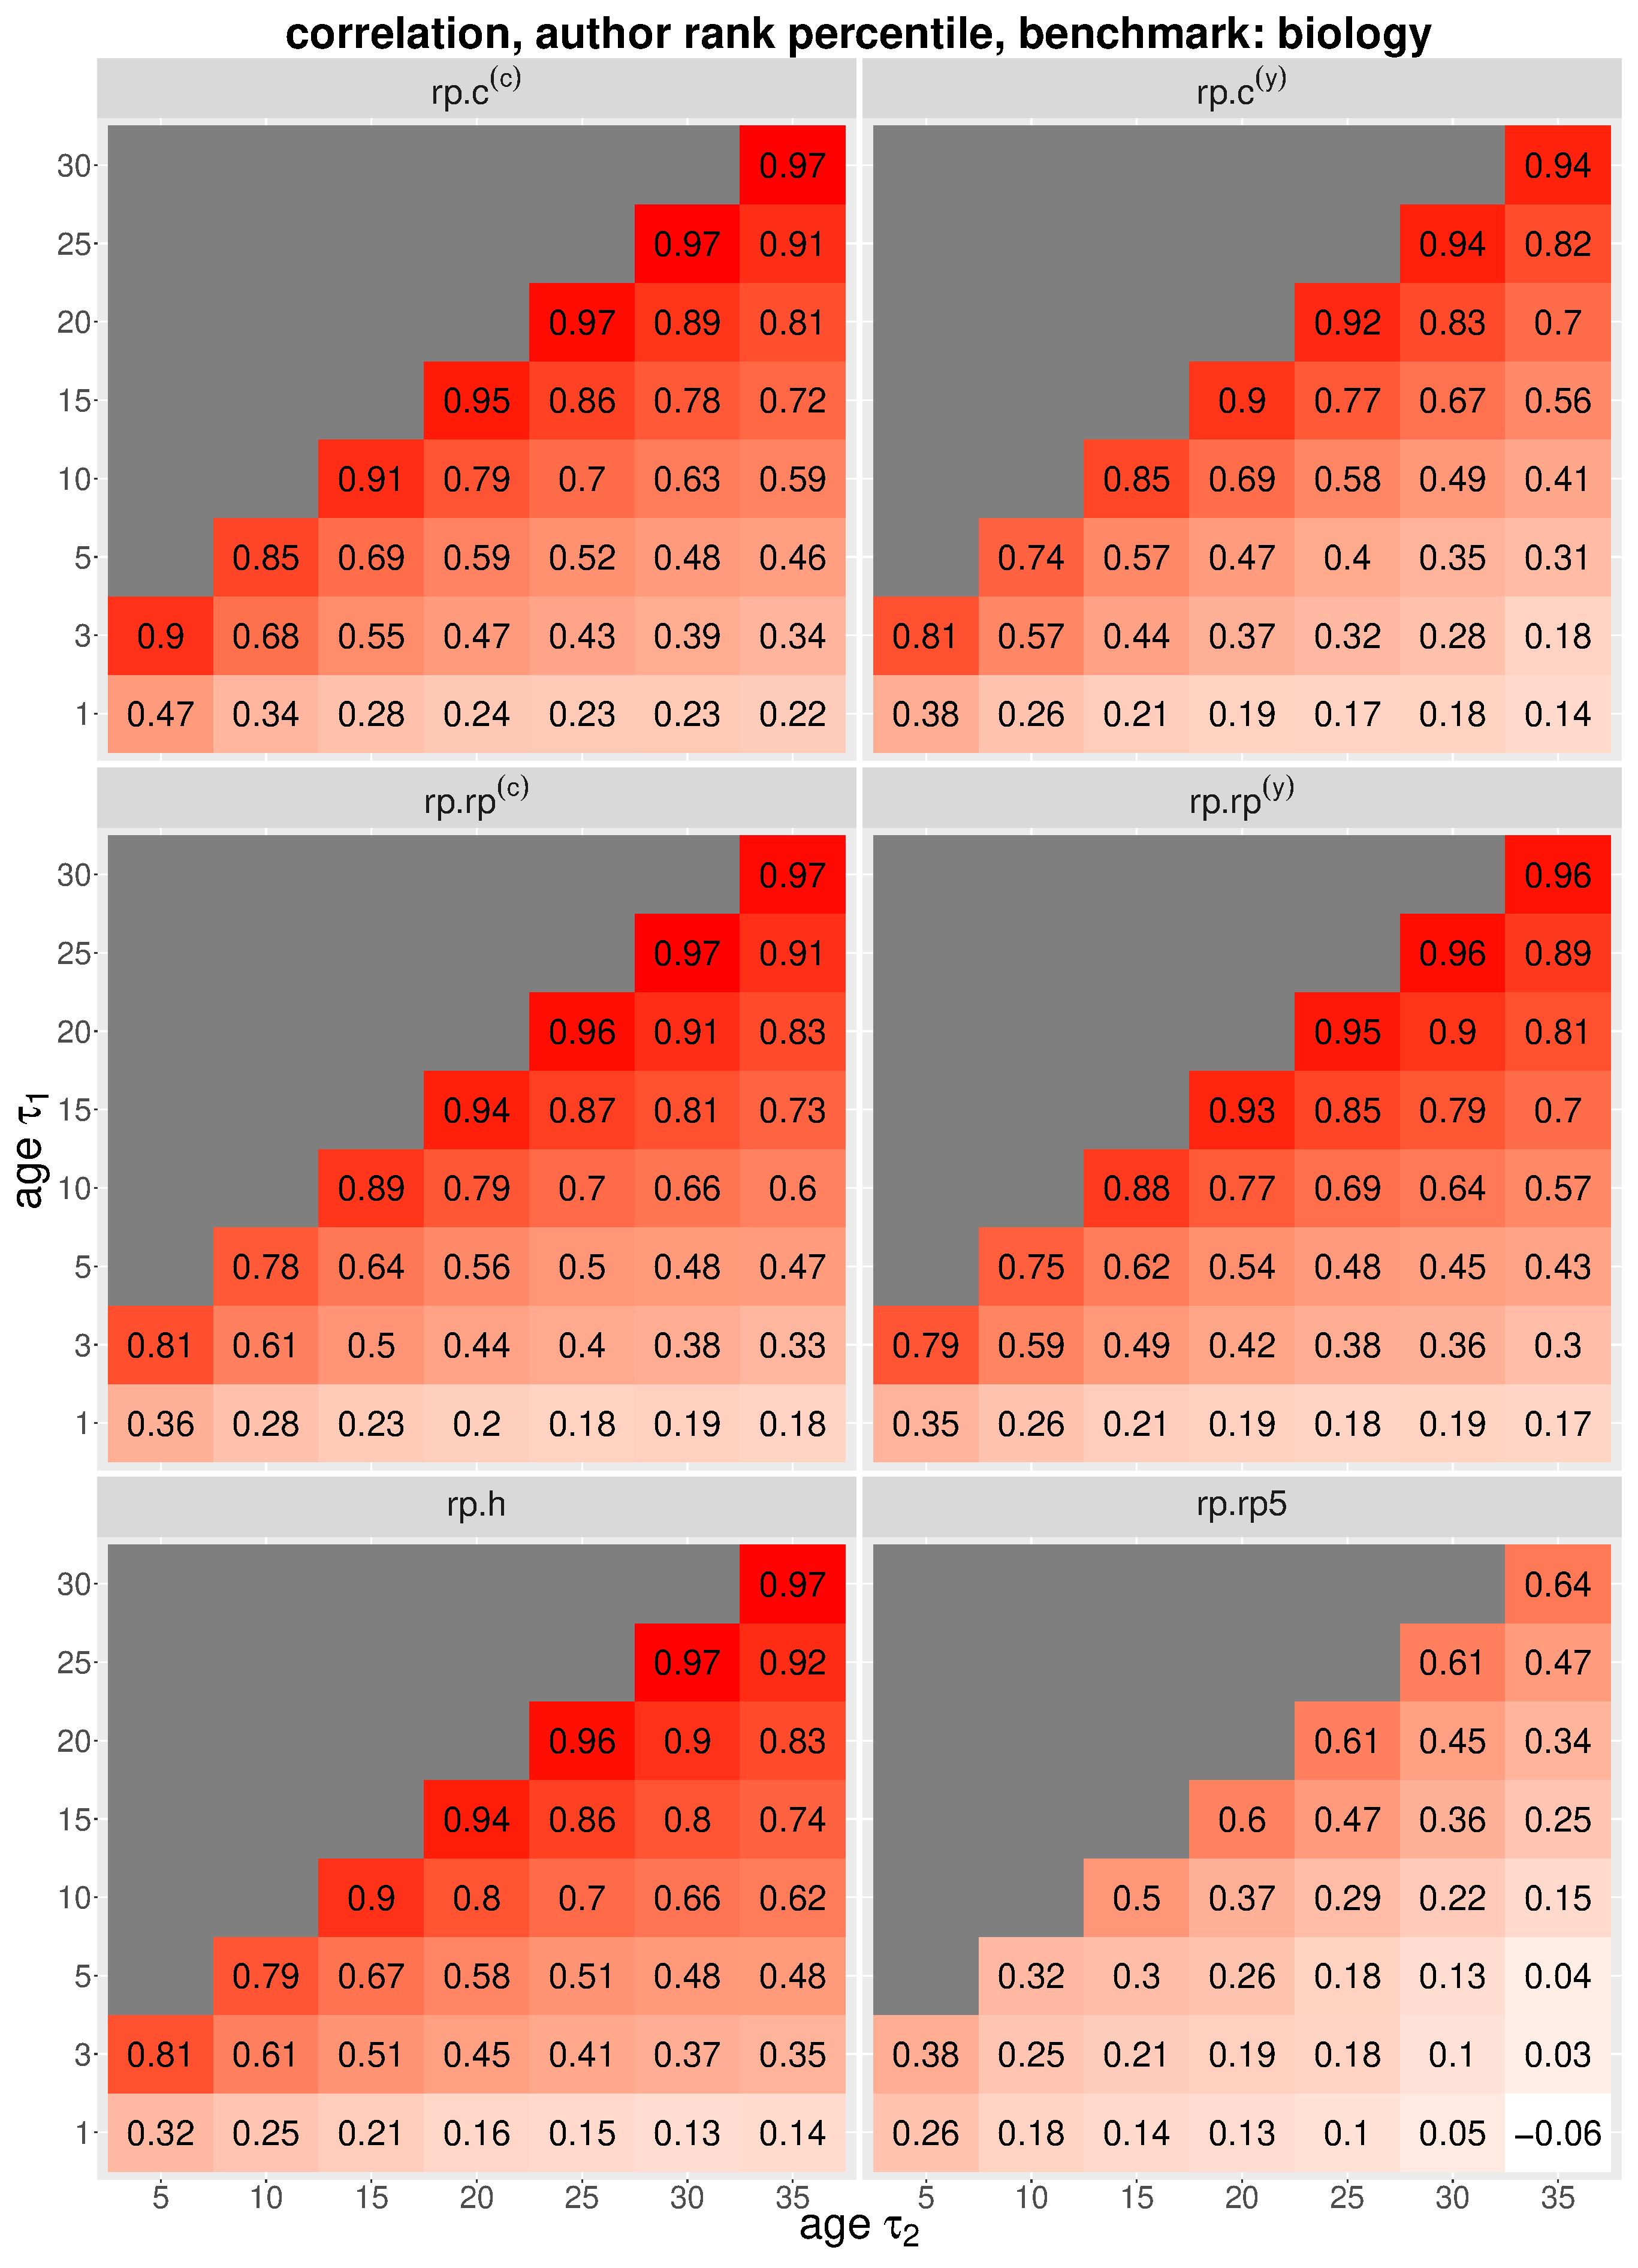
\includegraphics[width=\textwidth]{figures/pred_power/autrp/heatmap_cor_bio.eps}
    \caption{The Pearson's correlation between rp at two different ages, for various types of author rp. The benchmark includes only authors in biology.}
    \label{fig:hm_autrp_biology}
\end{figure}

\begin{figure}[ht!]
    \centering
    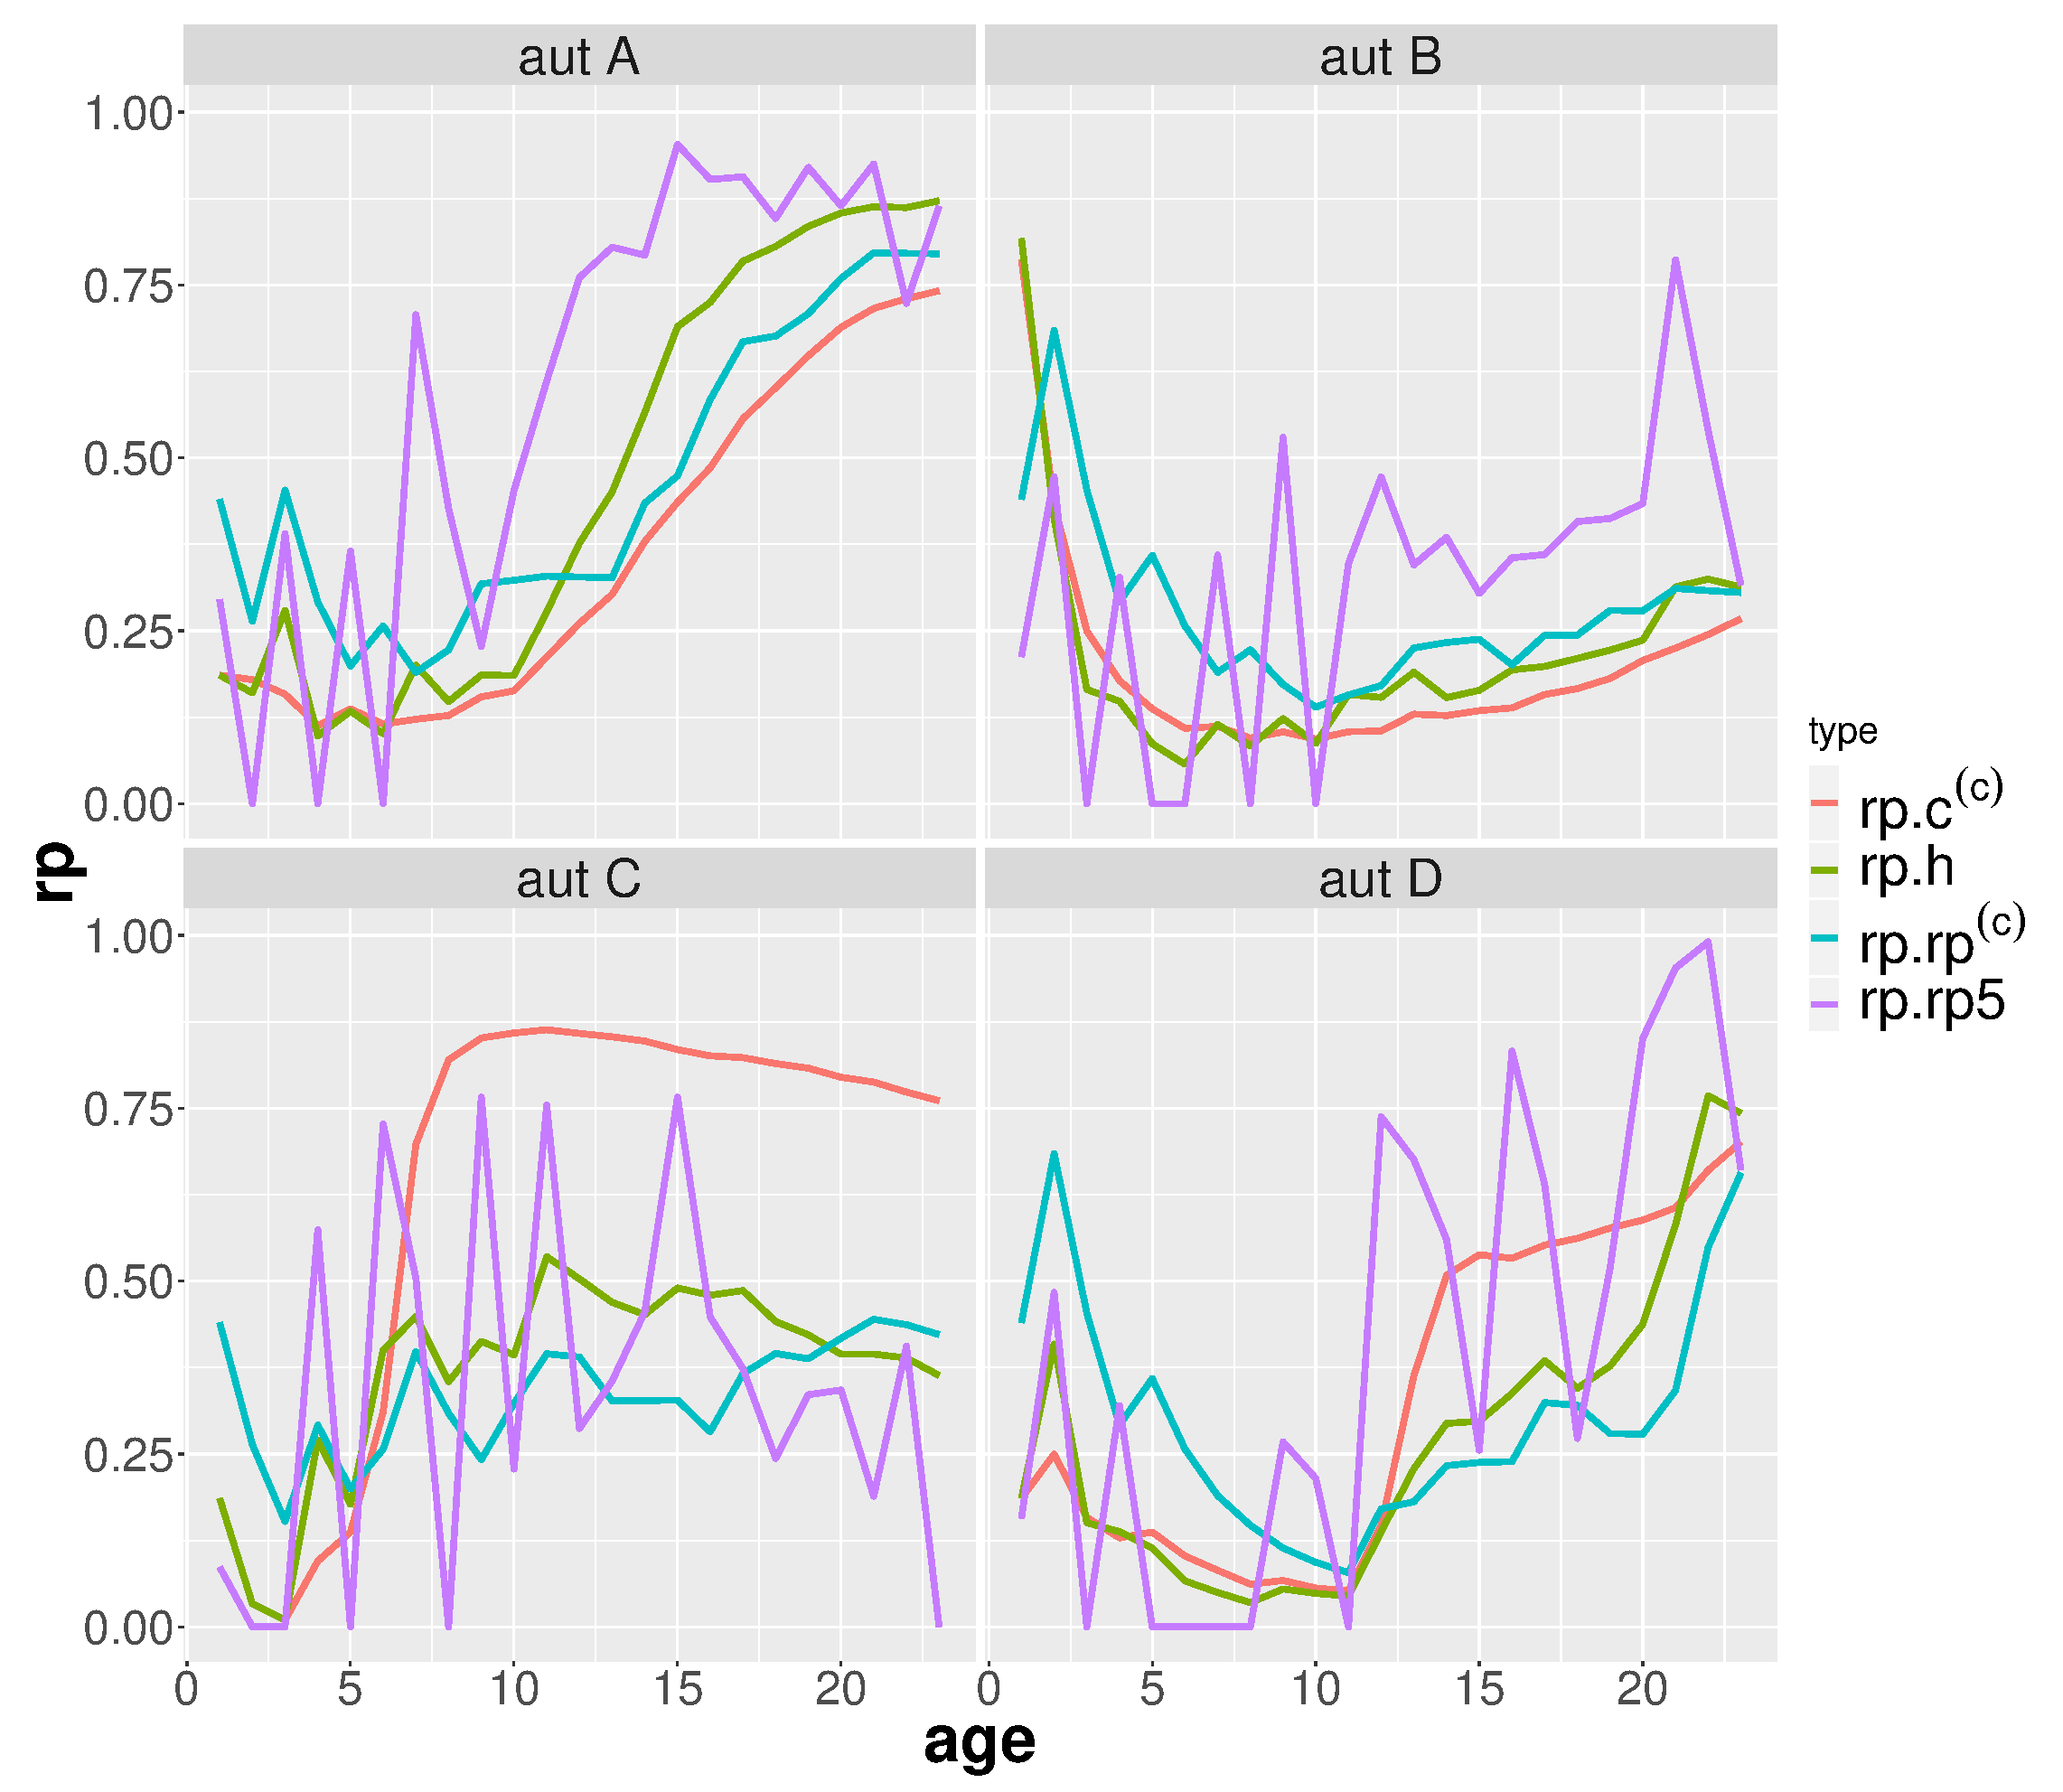
\includegraphics[width=\textwidth]{figures/exploratory/autrp_examples.eps}
    \caption{Examples of various types of author rank percentile over age. The $4$ authors shown in the figure have the same $\text{rp}^{(c)}_{i 5}$ and are all starting their careers from year $1990$. }
    \label{fig:aut_examples}
\end{figure}
\fi

\begin{figure}[ht!]
    \centering
    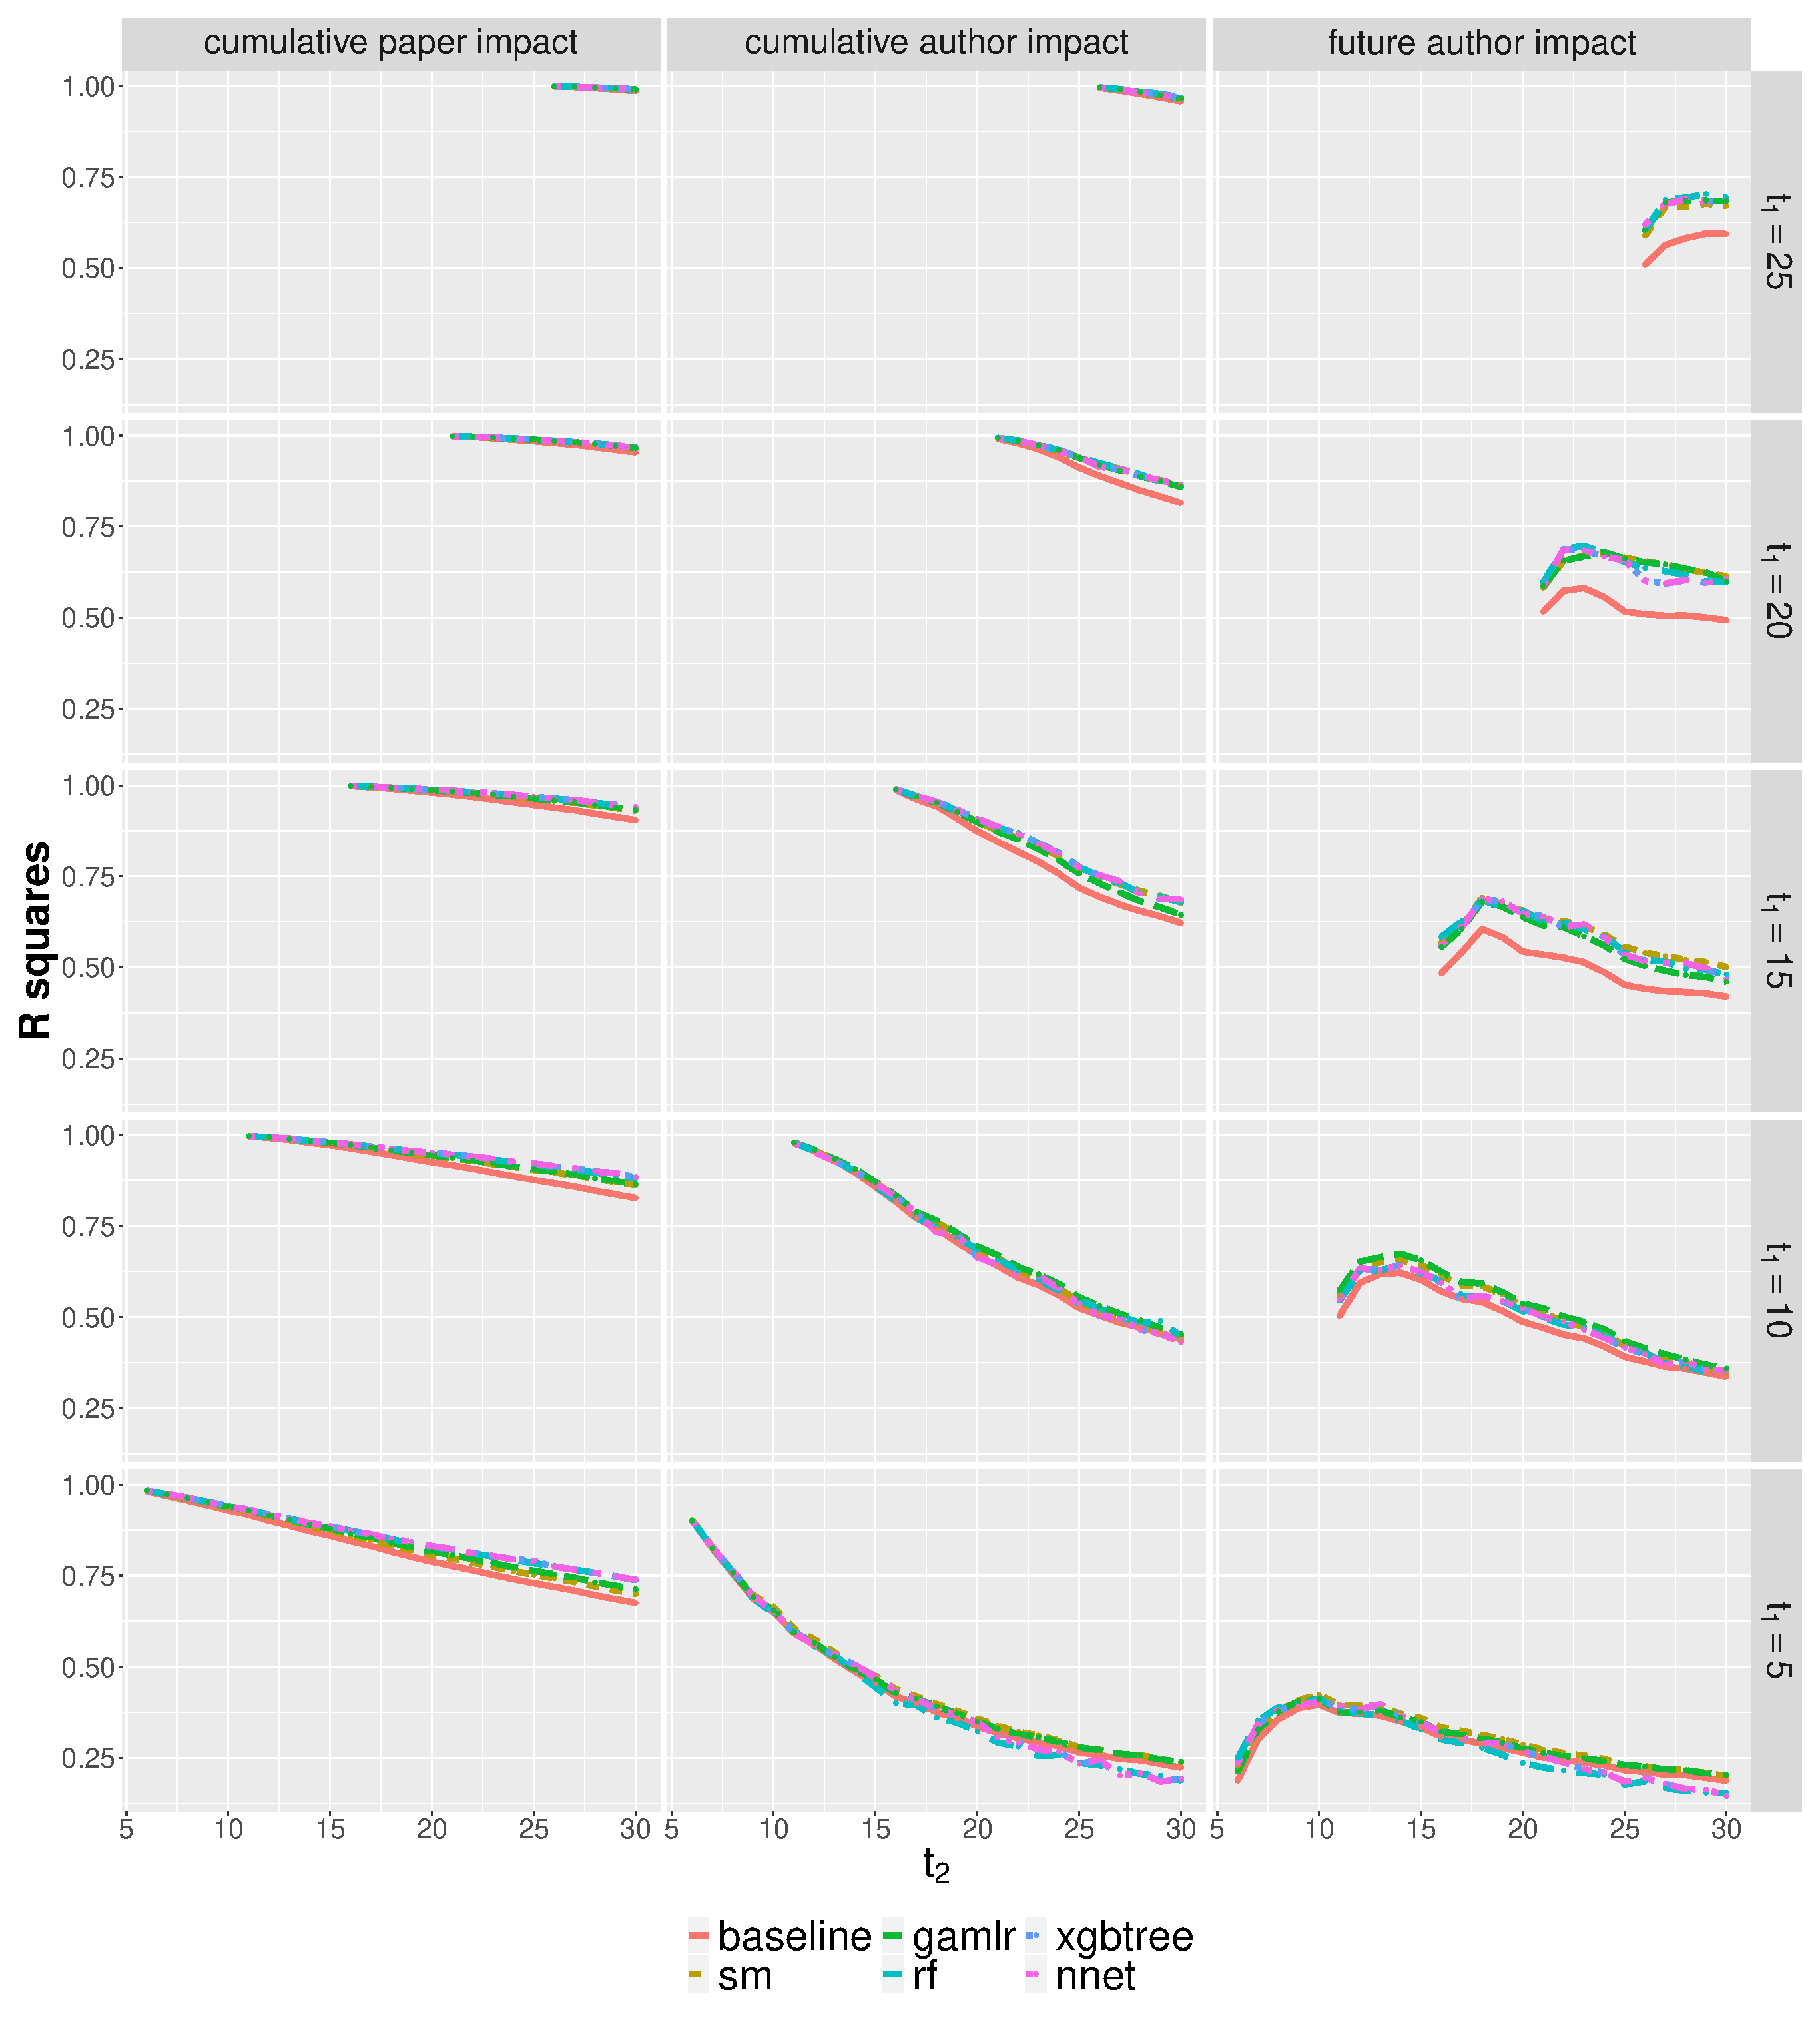
\includegraphics[width=\textwidth]{figures/pred_model/r2_diff.eps}
    \caption{Testing R squares of the predictive models. LASSO, ridge and elastic net are outperformed by Gamma LASSO, and hence are ignored for a better visualization.}
    \label{fig:pred_r2}
\end{figure}


\iffalse
\begin{figure}[ht!]
    \centering
        \begin{subfigure}[t]{0.8\textwidth}
        \centering
        \includegraphics[width=\textwidth]{figures/pred_model/pub/bio/importance.pdf}
        \caption{Top 5 features for predicting publication rp}
    \end{subfigure}%
    
    \begin{subfigure}[t]{0.8\textwidth}
        \centering
        \includegraphics[width=\textwidth]{figures/pred_model/aut/all/importance.pdf}
        \caption{Top 5 features for predicting author rp}
    \end{subfigure}

    \caption{Random permutation importance of features for predicting rank percentiles given by the random forest models. The top 5 features are selected based on the median of their importance values. }
    \label{fig:pred_model_importance}
\end{figure}
\fi



%!TEX root = ms.tex
\clearpage
\begin{refsection}
%\renewcommand*{\thepage}{A\arabic{page}}
\beginsupplement
\appendix
\pagenumbering{arabic}
\begin{center}
\textbf{\large Supplemental Material: \\ On the usage of rank percentile in evaluating and predicting the scientific impact}

Sen Tian, Panos Ipeirotis
\end{center}

\section{Rank percentile indicators for scholars}
\label{sec:suppl_similarity_autrp}

We consider the benchmark being the area of biology. In order to study the agreement of various indicators, for each indicator, we classify the scholars into four classes, class $1$: $0\le \text{S}_m^{ib}(t) < 0.25$, class $2$: $0.25\le \text{S}_m^{ib}(t) < 0.5$, class $3$: $0.5 \le \text{S}_m^{ib}(t) < 0.75$ and class $4$: $0.75 \le \text{S}_m^{ib}(t) \le 1$. An agreement is when two (or three) different indicators belong to the same class. The overall agreement for all three indicators, S$_{P5}$, S$_c$, and S$_h$, is $51\%$ at age $5$ and $68\%$ at age $30$; that is, for about half of the scholars the three indicators agree with each other at age $5$, while that number becomes around two third at age $30$. Figure \ref{fig:aut_rp_class} displays pairwise agreement of the three indicators. We see that the agreement increases with the age. Furthermore, S$_{P5}$ has large agreement with both S$_{c}$ and S$_{h}$, which are $69\%$ and $67\%$, respectively, at age $5$, and $71\%$ and $81\%$, respectively, at age $30$. 

Figure \ref{fig:hm_autrp_current} shows the correlation between S$_c^{ib}(t_1)$ and S$_c^{ib}(t_2)$, and the correlation between S$_h^{ib}(t_1)$ and S$_h^{ib}(t_1)$. The magnitudes of correlations are similar to those for S$_{P5}$ as shown in Figure \ref{fig:hm_rp_aut}.

% fig:aut_rp_class
% class agreement among all the author rp
\begin{figure}[ht!]
    \centering
    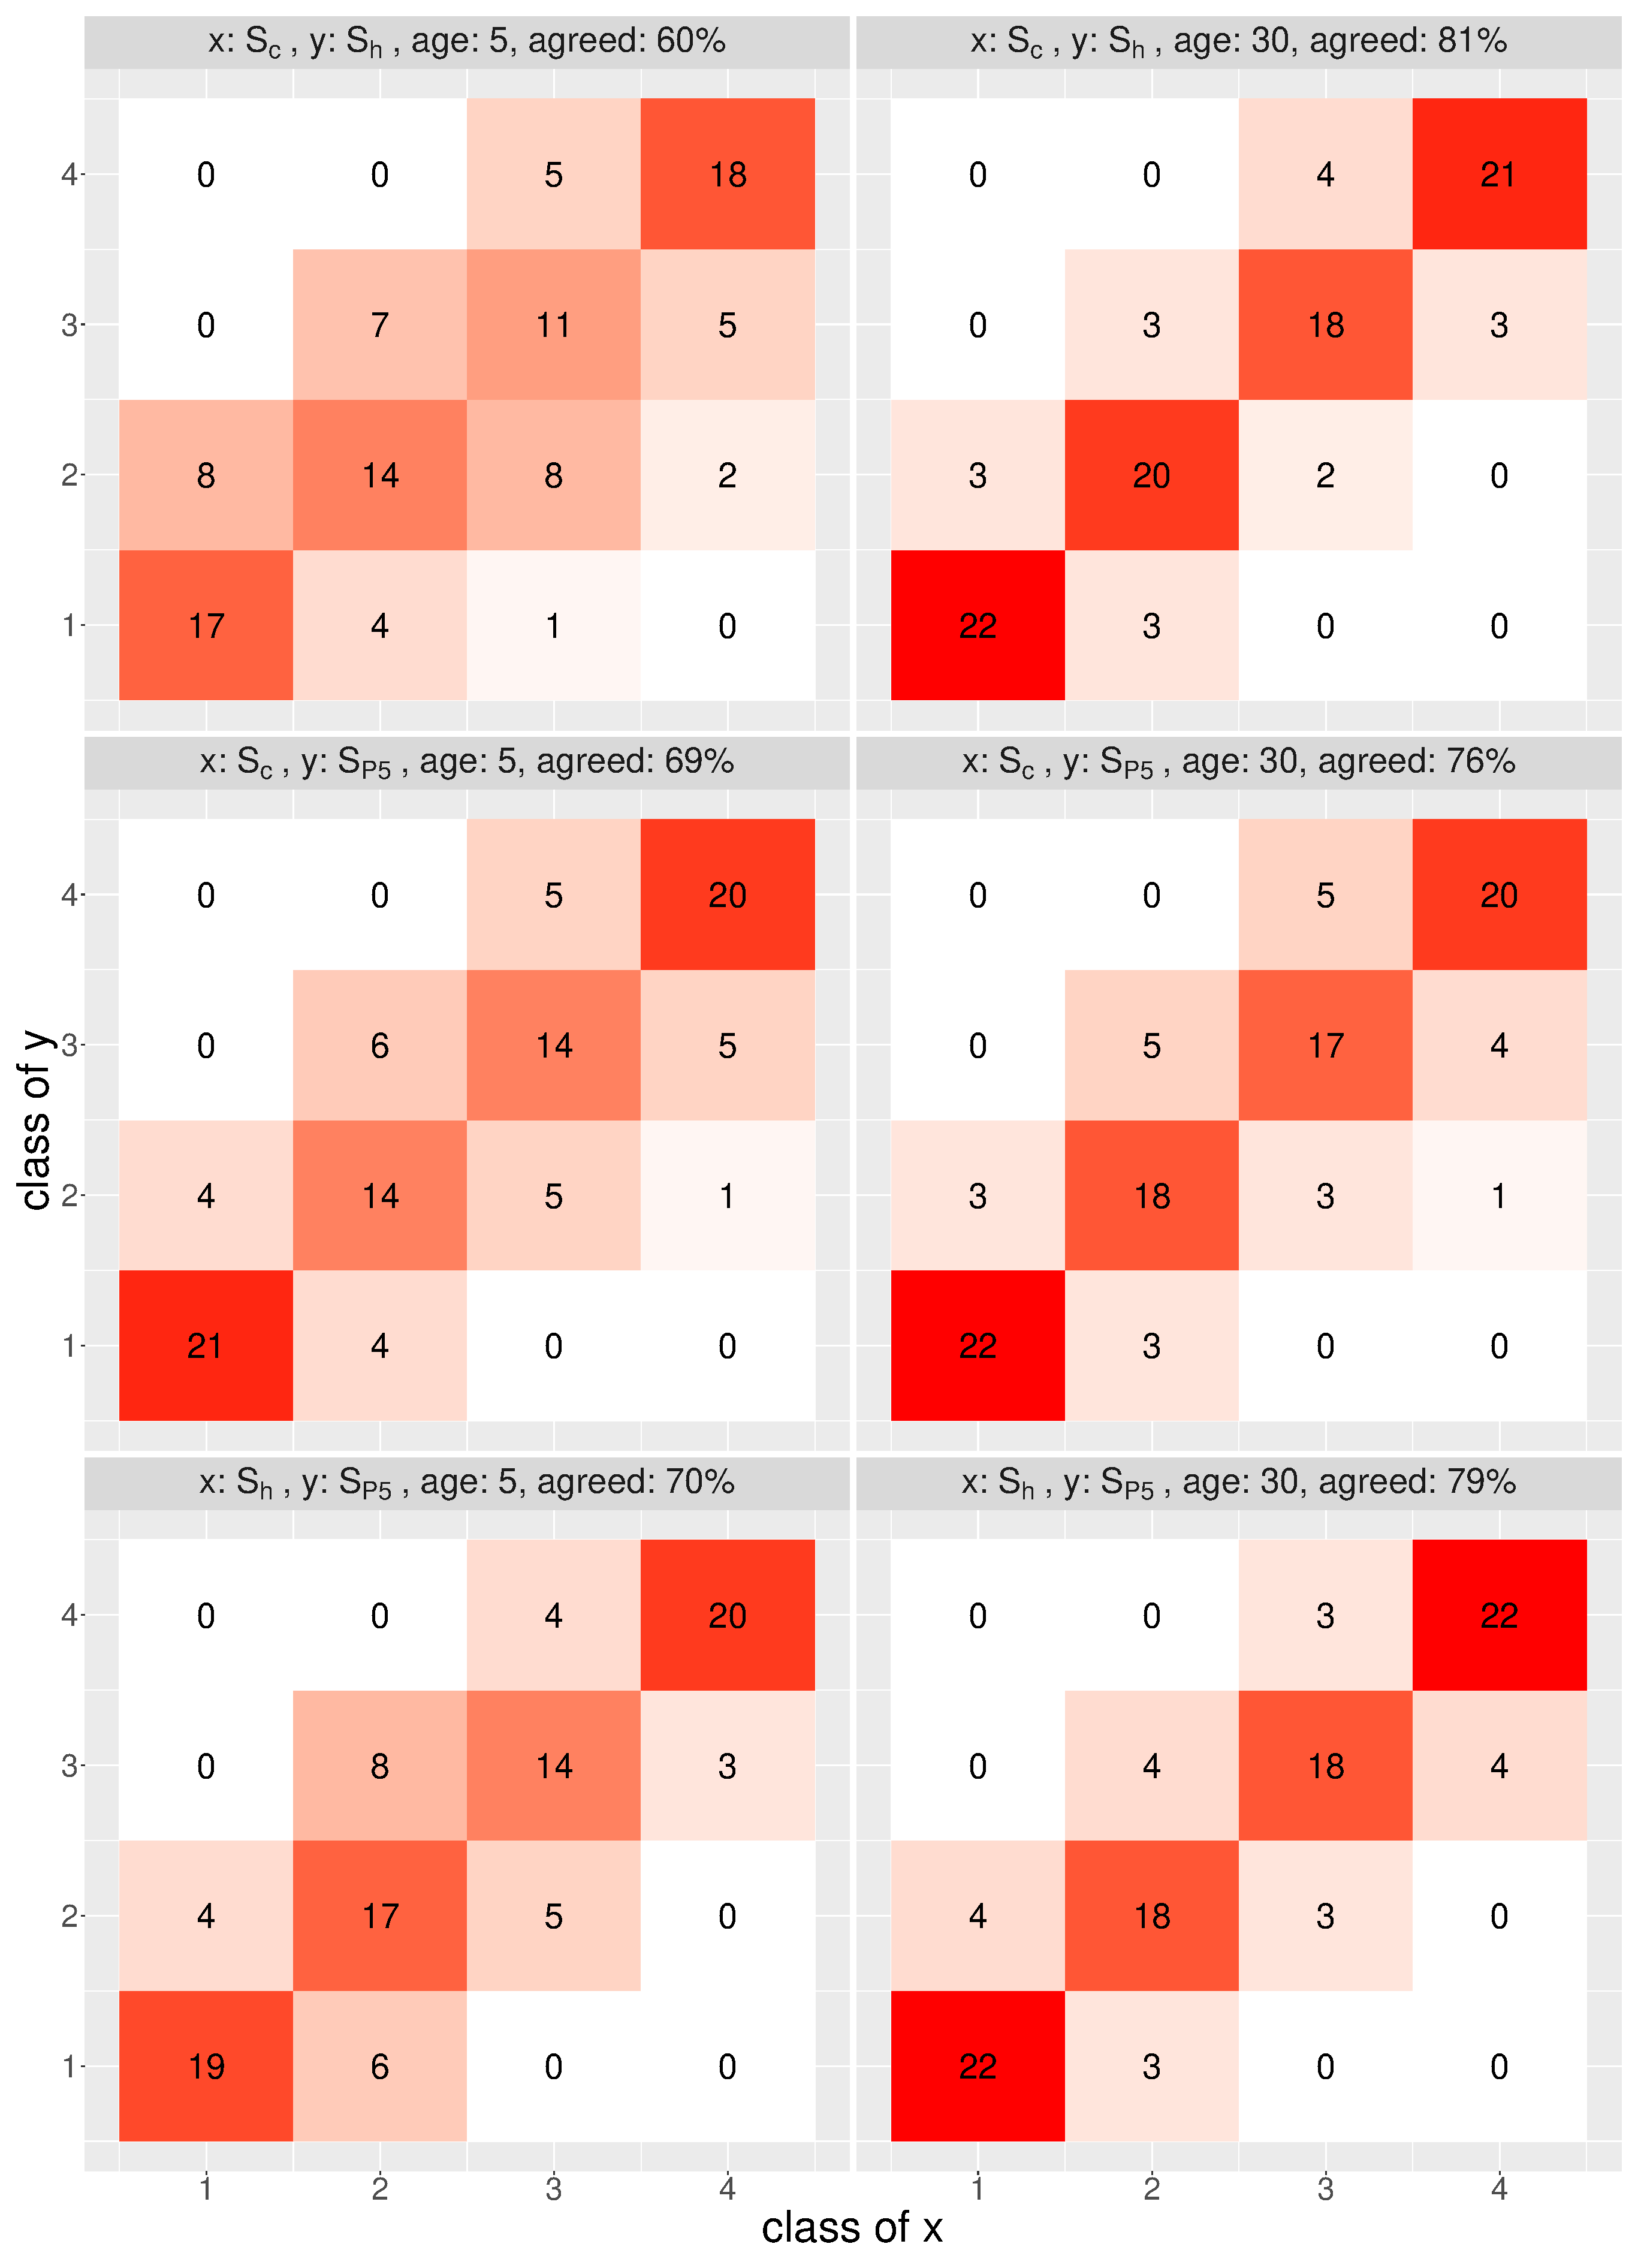
\includegraphics[width=0.88\textwidth]{figures/compare_autrp/heatmap_class_agreement.eps}
    \caption[The agreement of rank percentile indicators for scholars]{Rank percentile indicators are classified into four groups, that are class $1$: $0 \le \text{S}_m^{ib}(t) < 0.25$, class $2$: $0.25 \le \text{S}_m^{ib}(t) < 0.5$, class $3$: $0.5 \le \text{S}_m^{ib}(t) < 0.75$ and class $4$: $0.75 \le \text{S}_m^{ib}(t) \le 1$. The agreement of classes (sum of the anti-diagonal elements) is displayed in the title of each panel. The benchmark is biology. The agreement for all three indicators is $51 \%$ at age $5$ and is $68 \%$ at age $30$.}
    \label{fig:aut_rp_class}
\end{figure}

% publication rank percentile, heat map of correlations
\begin{figure}[ht!]
    \centering
    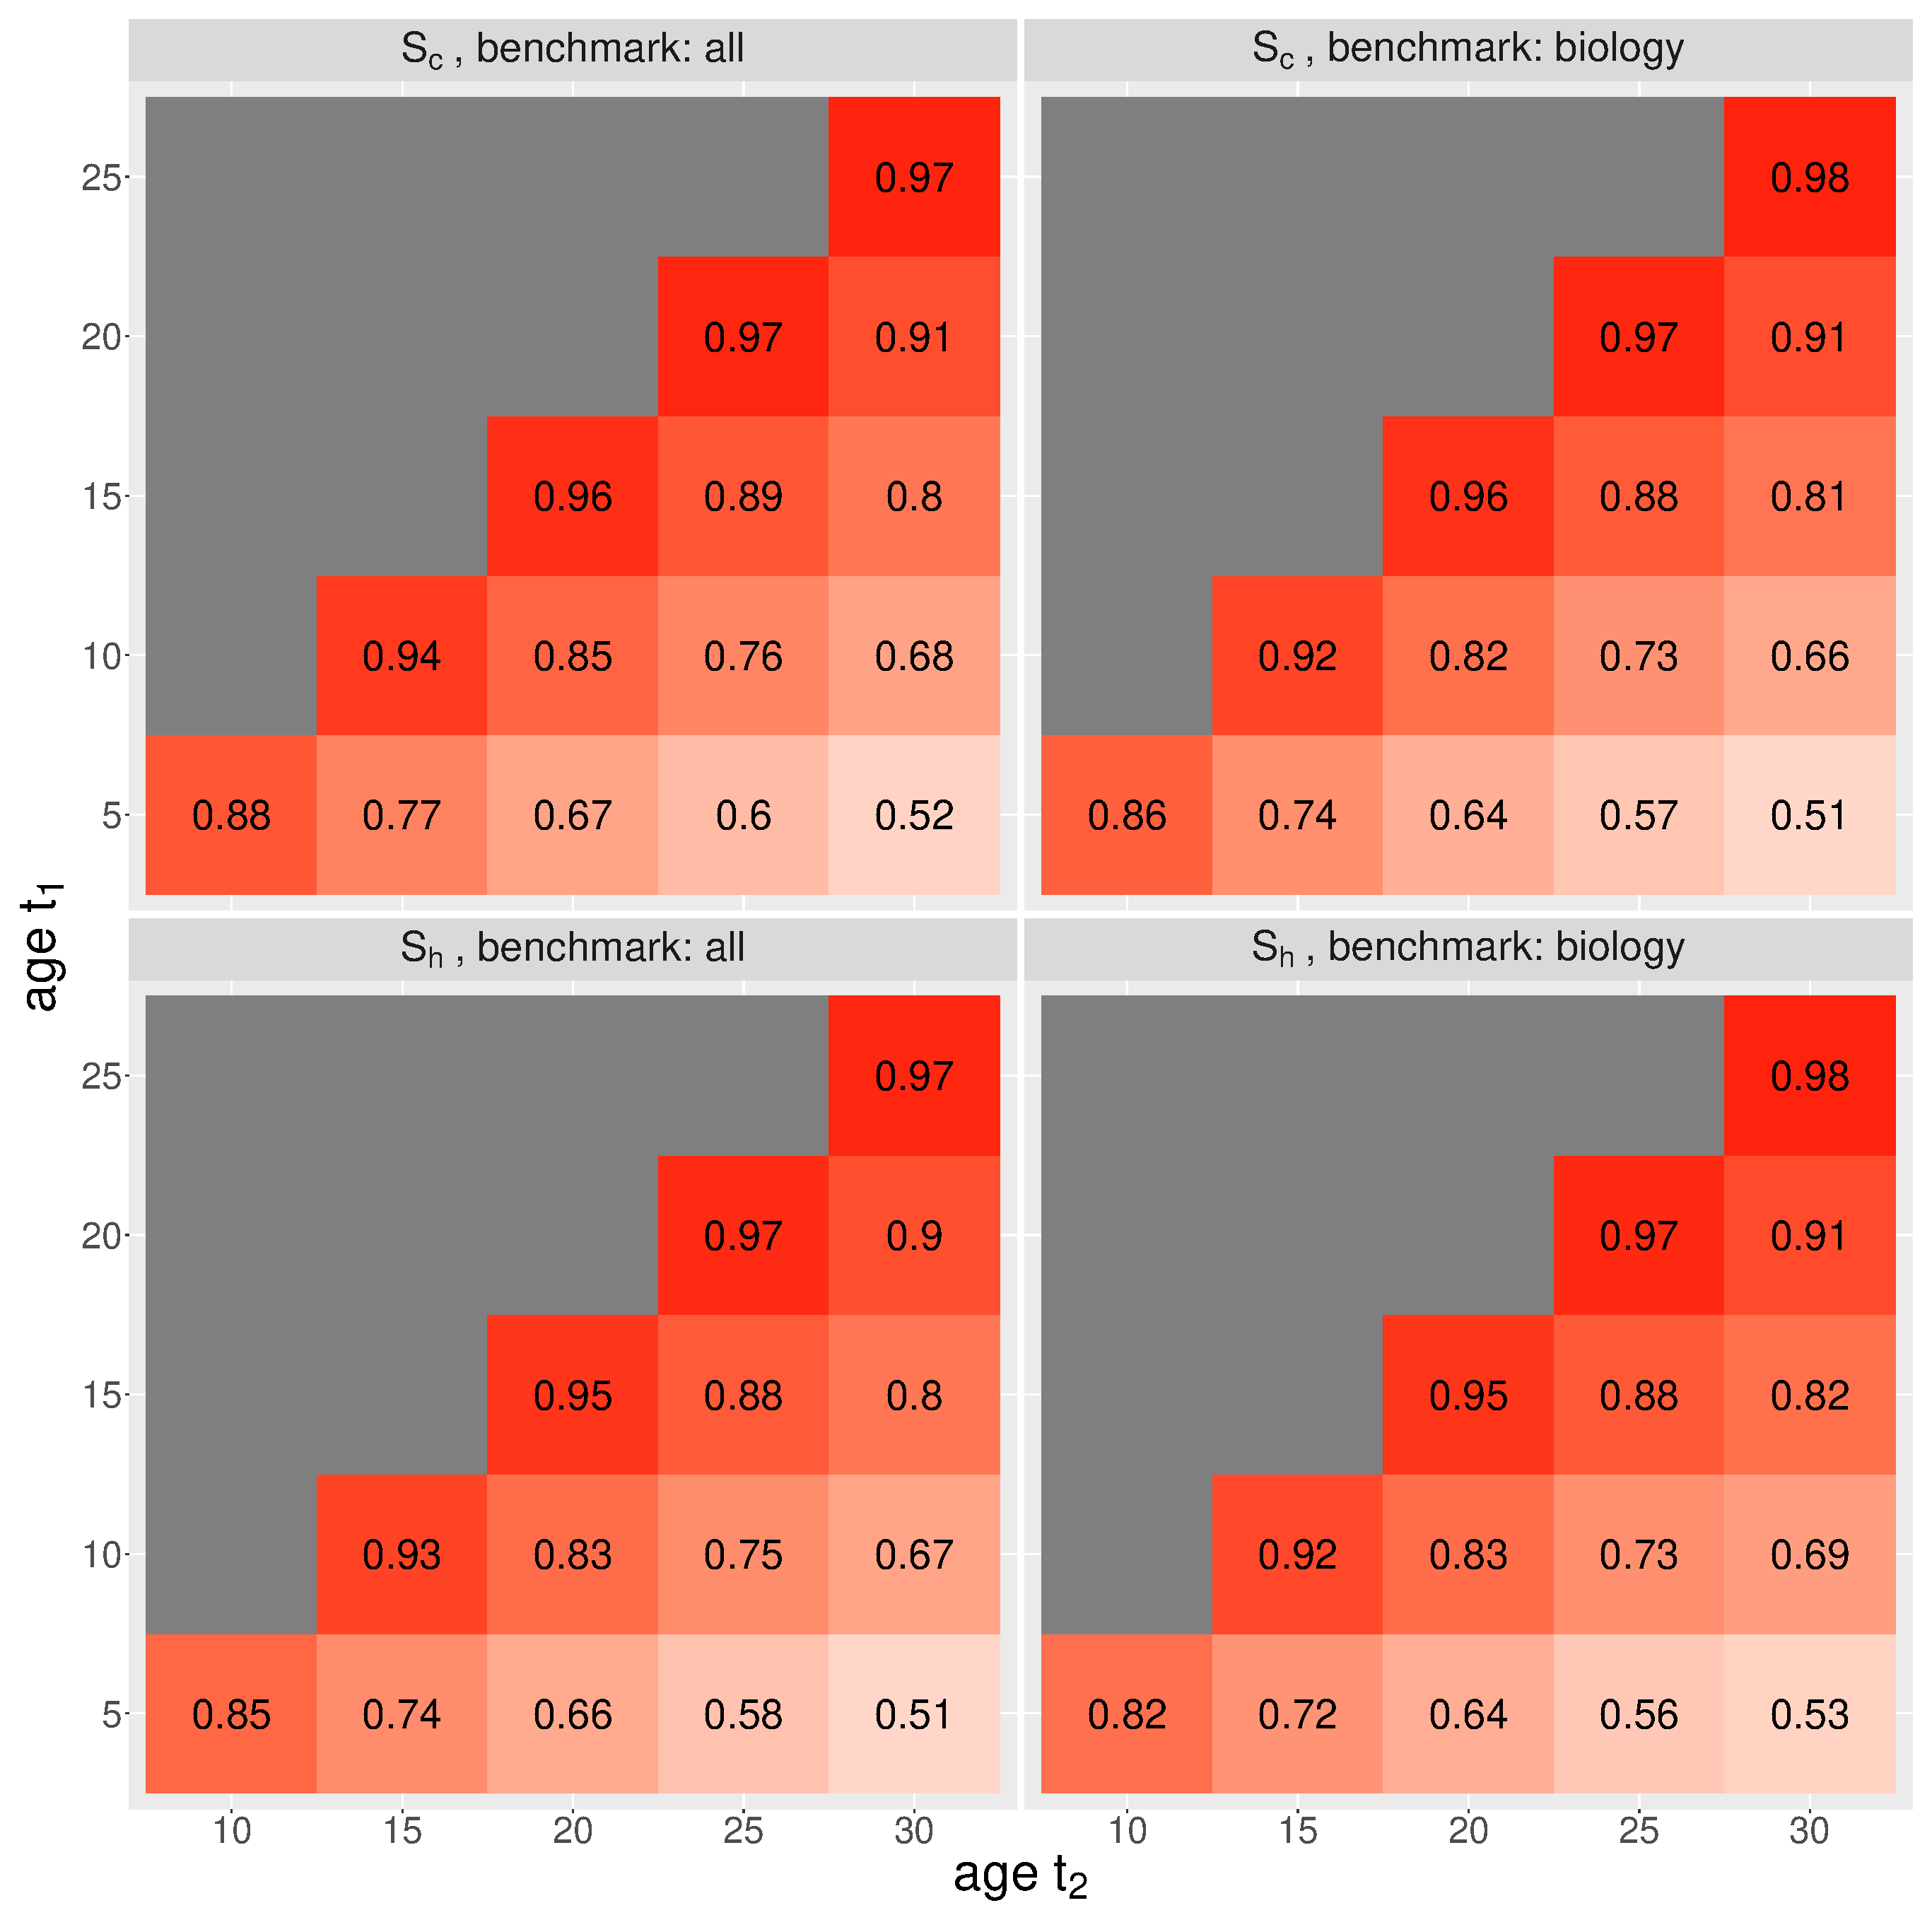
\includegraphics[width=\textwidth]{figures/pred_power/suppl_heatmap_cor_current.eps}
    \caption[Correlation heatmap for S$_c$ and S$_h$.]{The Pearson's correlation between rank percentile indicators at two different ages. }
    \label{fig:hm_autrp_current}
\end{figure}



\section{Robustness of \texorpdfstring{S$_{P5}$}{Lg}}
\label{sec:suppl_robustness_P5}

Recall that S$_{P5}^{ib}(t)$ is calculated based on an aggregation of the performances of publications that scholar $i$ publishes by age $t$. Denote $\text{m}_{P5}^{ib}(t)$ as the evaluation metric of scholar $i$ at age $t$ based on $\text{P}_{c}^{jb}(5)$, that is $\text{m}_{P5}^{ib}(t)= \sum_{j=1}^{N(t)} \text{P}_{c}^{jb}(5)$, where $N(t)$ is the total number of publications of scholar $i$ by age $t$. We illustrated in the paper that P$_c$ exhibits high stability, and hence P$_{c}^{jb}(5)$ can be applied to represent the performance of the publication. 

We further demonstrate the robustness of S$_{P5}$ by considering a longer citation history for each publication. Figure \ref{fig:robustness_test_cor} illustrates that m$_{P5}$ is highly correlated with m$_{P10}$ at age $t=1,\cdots,30$, where $\text{m}_{P10}^{ib}$t$= \sum_{j=1}^{N(t)} \text{P}_{c}^{jb}(10)$. We also consider the maximum, mean and median values of $\text{P}_{c}^{jb}(t)$, e.g. $\text{m}_{Pmax}^{ib}$t$= \sum_{j=1}^{N(t)} \max_{t^\prime}\text{P}_{c}^{jb}(t^\prime)$. We see from the figure that these metrics also exhibit high correlations with m$_{P5}$. Furthermore, we perform a Wilcoxon paired signed-rank test to compare the differences between S$_{P5}$ and S$_{P10}$ at each age $t=1,\cdots,30$, and the p-values are close to $1$; indicating that the differences are not statistically significant. Similar conclusions can be drawn for other indicators being considered.

\begin{figure}[ht!]
    \centering
    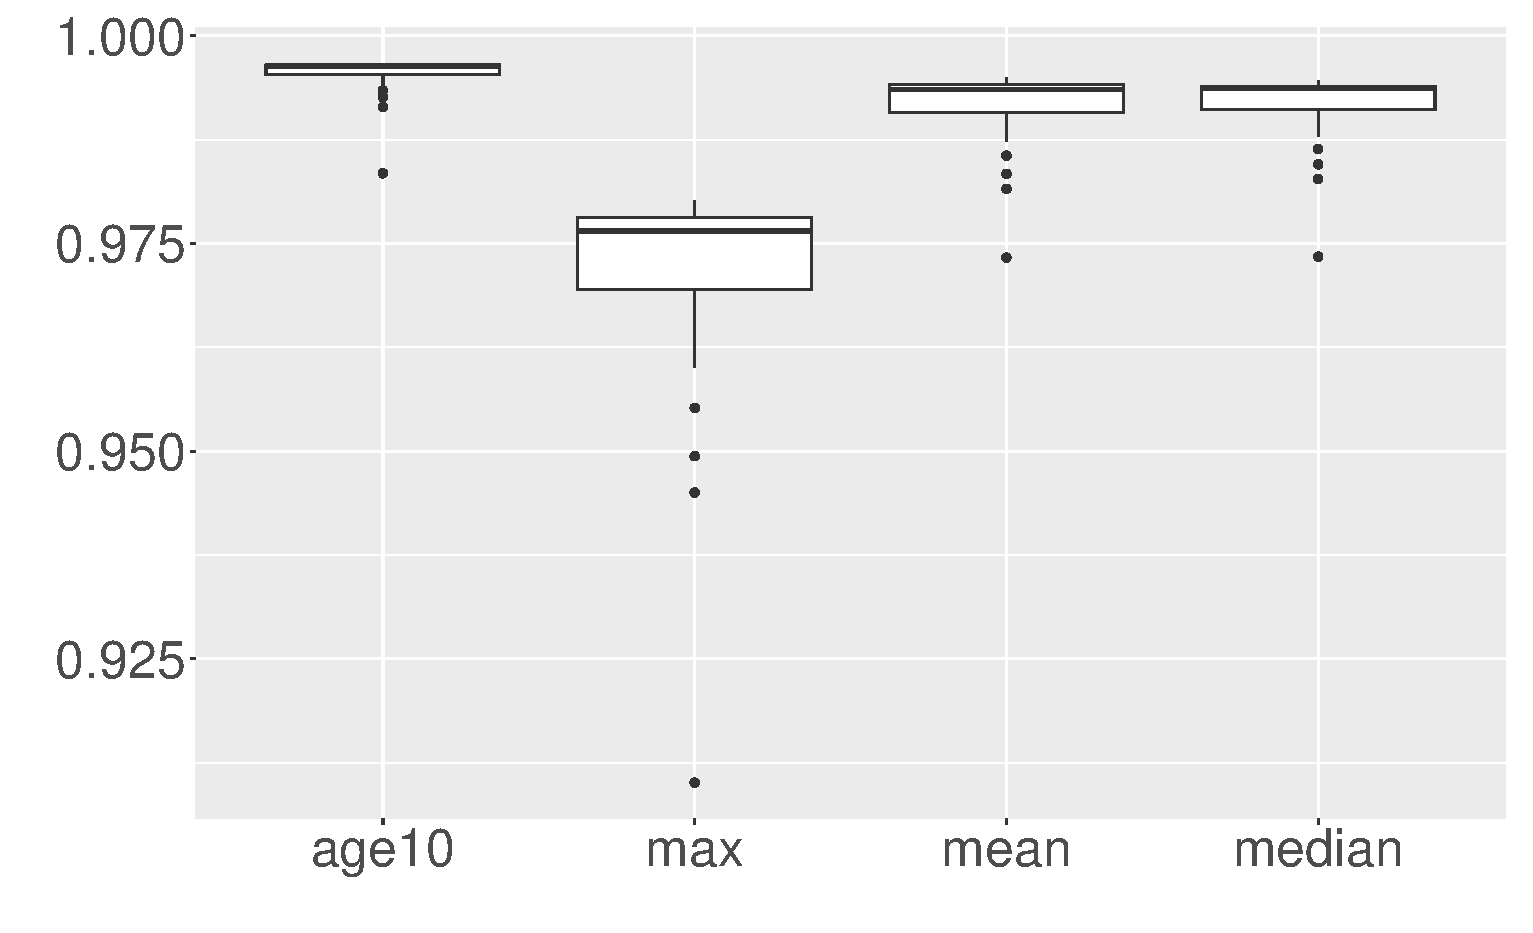
\includegraphics[width=0.7\textwidth]{figures/robustness/cor.eps}
    \caption[Correlation between m$_{P5}$ and other choices of evaluation metric]{Pearson's correlation between m$_{P5}$ and other choices of evaluation metric. Age $10$, max, mean and median correspond to m$_{P10}$, m$_{Pmax}$, m$_{Pmean}$ and m$_{Pmedian}$, respectively. The correlation is calculated at each age $t=1,\cdots,30$.}
    \label{fig:robustness_test_cor}
\end{figure}


\iffalse
\begin{equation}
\label{eq:rp_matrix}
\bordermatrix{
    & \text{age 1}     & \text{age 2}     & \cdots & \text{age $K$}     \cr
    \text{paper 1}     & \text{rp}_{11}^{(c)}     & \text{rp}_{12}^{(c)}     & \ldots & \text{rp}_{1 K}^{(c)}      \cr
    \text{paper 2}     & \text{rp}_{21}^{(c)}     & \text{rp}_{22}^{(c)}    & \ldots & \text{rp}_{2 K}^{(c)}     \cr
    \quad \vdots & \vdots & \vdots & \ddots & \vdots \cr
    \text{paper $N$}     & \text{rp}_{N 1}^{(c)}     & \text{rp}_{N 2}^{(c)}     & \ldots  & \text{rp}_{N K}^{(c)}    \cr
}
\end{equation}

We take the maximum performance for each of the $N$ papers, and sum them:
\begin{equation}
    \omega_{i \tau} = \sum_{j=1,\cdots,N} \max_{k=1,\cdots, K} \text{rp}_{j k} ^{(c)}.
\end{equation}
\fi

\section{Stationarity test}
\label{sec:suppl_stationarity}

Two commonly used statistical tests for stationarity are the Dicky-Fuller test~\cite{dickey1979distribution} and KPSS test~\cite{kwiatkowski1992testing}. These two tests formulate the hypothesis testing problems differently. Dicky-Fuller test assumes a unit root presented in the series. A unit root means that the series is $I(1)$, i.e. integrated order $1$ and the first differenced series is stationary. The more negative the test statistic is, the stronger the rejection of the null. On the other hand, KPSS test assumes the null as the series being stationary, i.e. $I(0)$. KPSS test is slightly more general since it allows testing a series being non-stationary but does not present a unit root. The more positive the test statistic is, the stronger the rejection of the null. Both tests include the drift in the test equations but exclude the trend, since we do not observe significant trends in the series. 

The test statistics are shown in Figure \ref{fig:stationarity_test}. The dashed lines indicate the critical values at $5 \%$ level. KPSS test indicates that P$_c$ and S$_{P5}$ are non-stationary series, and we do not have enough evidence to reject them being $I(1)$ according to the Dicky-Fuller test. Furthermore, the differenced series are stationary based on both tests.


\begin{figure}[ht!]
    \centering
    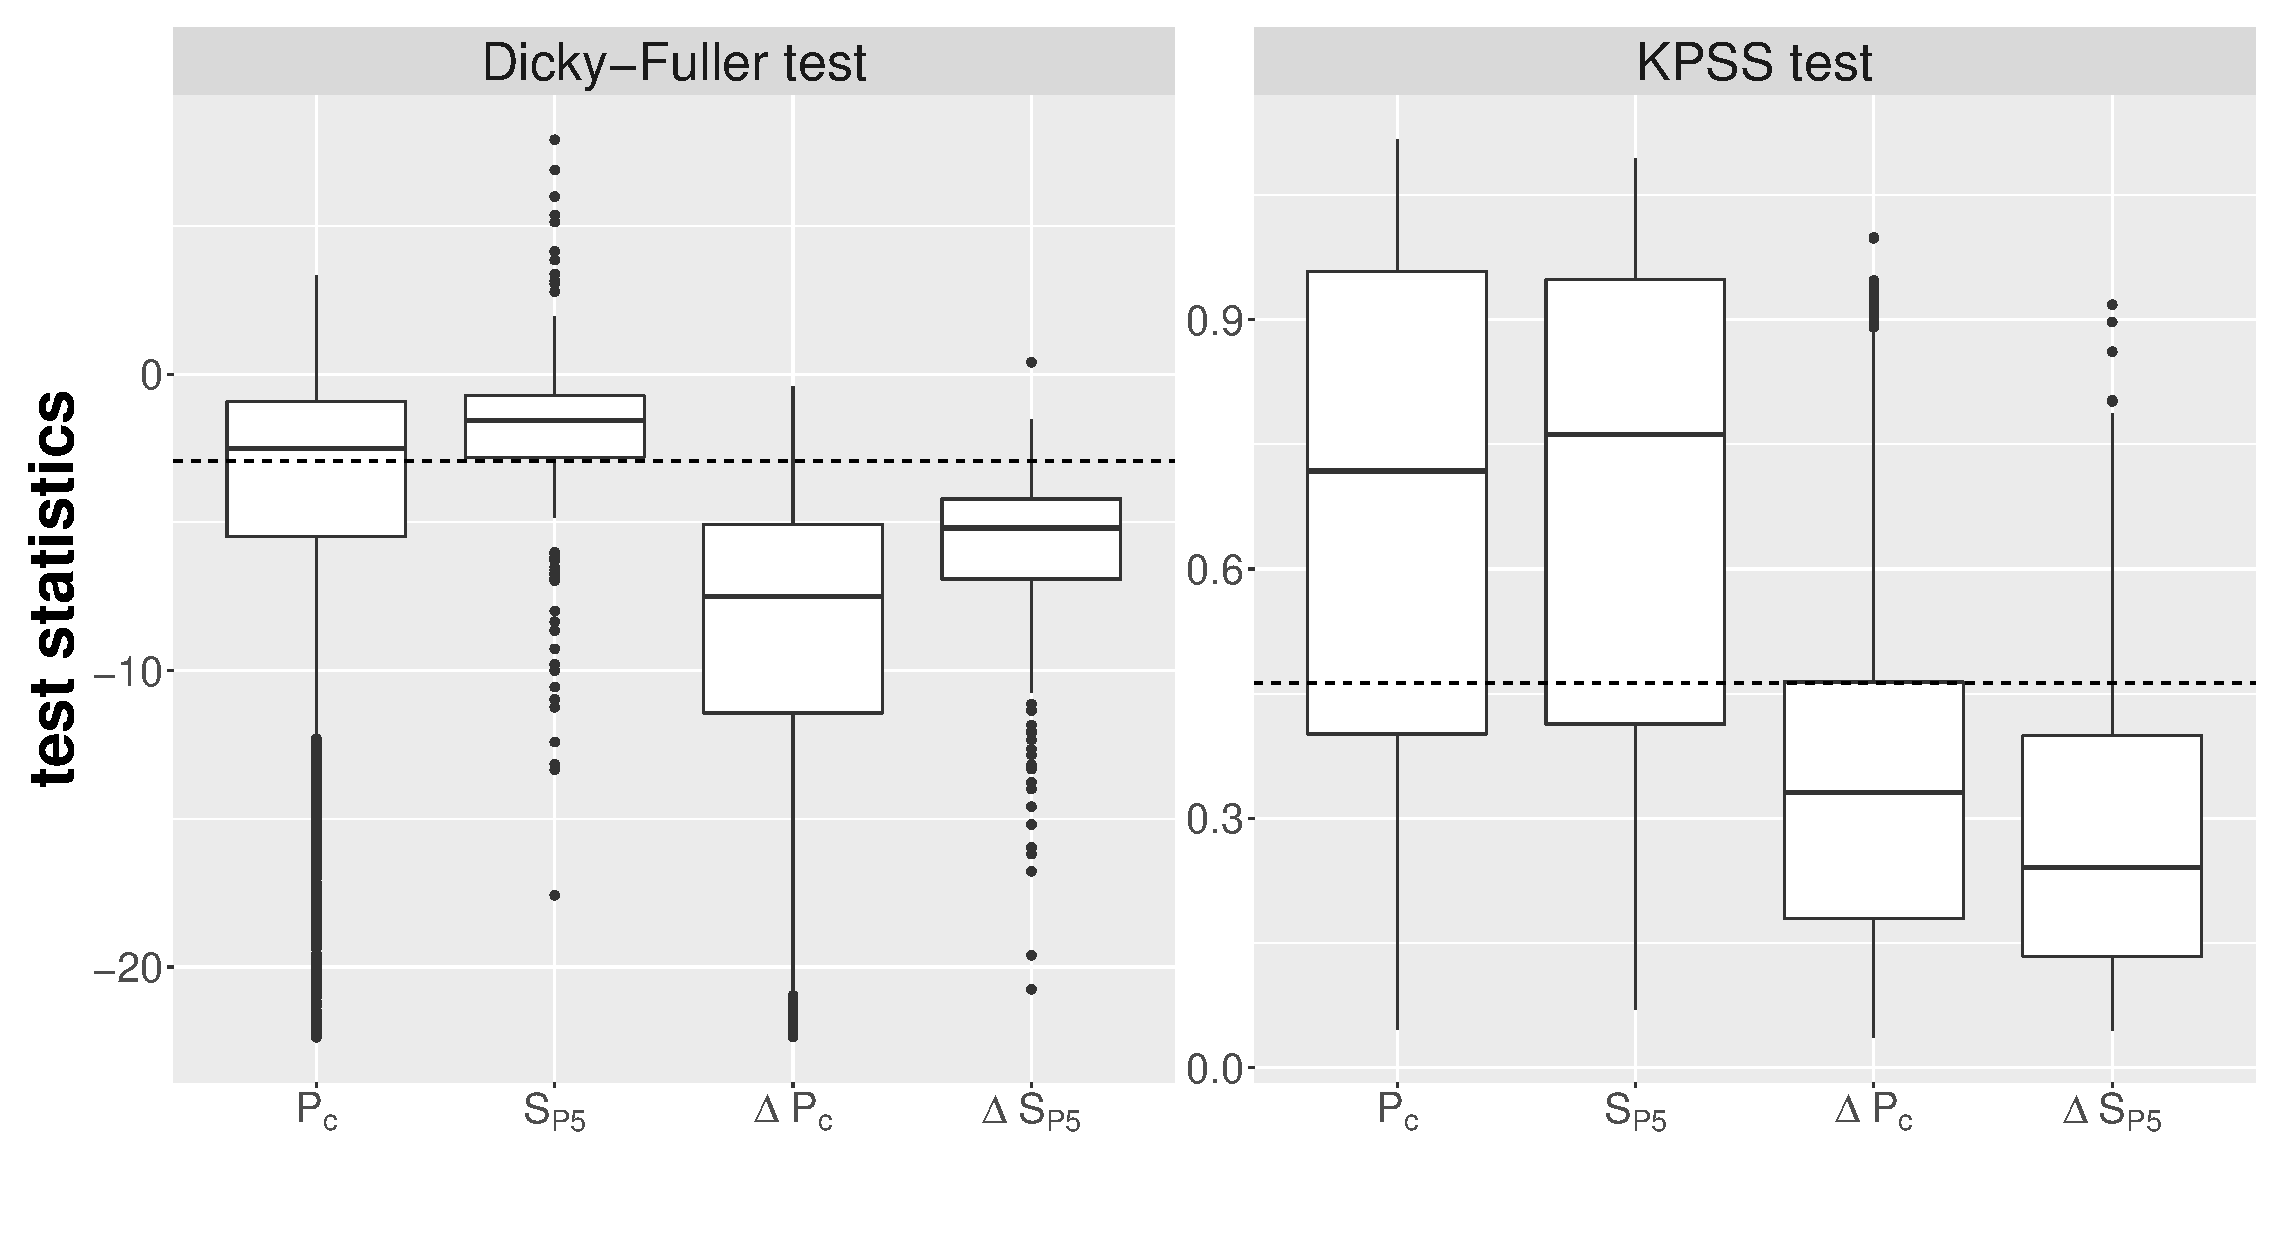
\includegraphics[width=\textwidth]{figures/stationarity/df_kpss.eps}
    \caption[Stationarity test of rank percentile series]{Statistical tests for the stationarity of rank percentile series. Both tests are applied on every individual series, and the test statistics are presented. The $5\%$ critical value for each test is illustrated by the dashed horizontal line. Both tests suggest that publication indicator P$_c$ and scholar indicator S$_{P5}$ are non-stationary, while their differenced series are stationary. }
    \label{fig:stationarity_test}
\end{figure}

\iffalse
\section{Details of the predictive models}
\label{sec:suppl_details_predmodel}

The details of the predictive models are described below.
\begin{itemize}
    \item Baseline: simple linear regression of P$_{it_2}^c$ on P$_{it_1}^c$. Same applies for S$_{it}^{P5}$.
    \item Simple Markov model (sm): linear regression of P$_{it_2}^c$ on P$_{it_1}^c$ and the change of P$_{it}^c$ over the last $2$ ages, i.e. P$_{it_1}^c$-P$_{it_1-2}^c$. Same applies for S$_{it}^{P5}$.
    \item Penalized linear regression models, including the ridge, lasso, elastic net (enet) and the Gamma lasso (gamlr): linear models with different penalties on the regression coefficients. All of these methods shrink the coefficients towards zero, and the later three methods can provide sparse solutions (shrink the coefficients to be exactly zeros). 
    \item Ensemble methods of regression trees, including the random forest (rf) and extreme gradient boosting trees (xgbtree): rf is a bagging of regression trees with a subset of randomly selected features chosen at each split to avoid overfitting. xgbtree is a fast implementation of gradient boosting on regression trees with a model formation that emphasizes the role of regularizations to avoid overfitting.
    %\item Support vector regression (svr)~\cite{drucker1997support}: 
    \item Neural networks (nnet): feedforward networks with multiple hidden layers, and using dropout and $l_2$ regularization to avoid overfitting.
\end{itemize}
\fi


\begin{table}[htbp]
  \centering
    \begin{tabular}{l|l}
    Method & Tuning parameters \\
    \midrule
    Lasso & Penalty strength parameter \\
    \midrule
    Ridge & Penalty strength parameter \\
    \midrule
    \multirow{2}[2]{*}{Elastic net} & Penalty strength parameter \\
          & Penalty gap parameter \\
    \midrule
    \multirow{2}[2]{*}{Gamma lasso} & Penalty strength parameter \\
          & Convexity parameter \\
    \midrule
    \multirow{3}[2]{*}{Random forest} & Number of trees to grow \\
          & Number of variables used at each split \\
          & Minimum number of observations in a node \\
    \midrule
    \multirow{9}[2]{*}{xgbtree} & Maximum number of iterations \\
          & Learning rate \\
          & Regularization parameter \\
          & Maximum depth of the tree \\
          & Minimum number of observations in each child leaf \\
          & Number of observations supplied to a tree \\
          & Number of features supplied to a tree \\
          & Regularization parameter for ridge penalty \\
          & Regularization parameter for LASSO penalty \\
    \midrule
    \multirow{5}[1]{*}{Deep neural network} & Number of layers  \\
          & Learning rate \\
          & Number of hidden units at each layer \\
          & Dropout rate \\
          & Regularization parameter \\
    \end{tabular}%
  \caption[Hyperparameter(s) of the machine learning models]{Hyperparameter(s) of the machine learning models.}
  \label{tab:hyperpara}%
\end{table}%

\begin{table}[htbp]
  \centering
    \begin{tabular}{l|l}
    Feature & Description \\
    \midrule
    pub\_cit\_cumulative & total citations of publication $j$ \\
    pub\_cit\_yearly & yearly citations of publication $j$ received in $t_1$ \\
    pub\_cit\_peryear & average citations of publication $j$ over age \\
    pub\_rp\_cumulative & rank percentile indicator calculated based on total citations, i.e. P$_c^{jb}(t_1)$ \\
    pub\_rp\_yearly & rank percentile indicator calculated based on yearly citations at $t_1$\\
          &  \\
    aut\_cit\_cumulative          & total citations of author $i$ \\
    aut\_cit\_yearly          & yearly citations of author $i$ at $t_1$ \\
    aut\_npub\_cumulative & total number of publications of author $i$ \\
    aut\_npub\_yearly & yearly number of publications of author $i$ at $t_1$ \\
    aut\_cit\_perpaper & average citations per paper for author $i$  \\
    aut\_h\_index & h-index of author $i$  \\
    aut\_g\_index & g-index of author $i$ \\
    aut\_maxcit\_pub & largest citation that a single paper of author $i$ has received \\
    aut\_rprp5\_cumulative & rank percentile calculated based on all papers, i.e. S$_{P5}^{ib}(t_1)$ \\
    aut\_rprp5\_yearly & rank percentile calculated based on just papers written at $t_1$ \\
          &  \\
    *\_delta & the difference over the last two ages for each of the above features \\
    \end{tabular}%
  \caption[Features for predicting the publication impact]{Features for predicting the impact of publication $j$ of scholar $i$. The features are created at $t_1$.}
  \label{tab:features_pubrp}%
\end{table}%

\begin{table}[htbp]
  \centering
    \begin{tabular}{l|l}
    Feature & Description \\
    \midrule
    aut\_cit\_cumulative & total citations of author $i$ \\
    aut\_cit\_yearly & yearly citations of author $i$ at age $t_1$ \\
    aut\_npub\_cumulative & number of publications of author $i$ \\
    aut\_npub\_yearly & yearly number of publications of author $i$ at age $t_1$ \\
    aut\_h\_index & h-index of author $i$ \\
    aut\_g\_index & g-index of author $i$ \\
    aut\_cit\_peryear & average citations per age of author $i$ \\
    aut\_rprp5\_cumulative & rank percentile calculated using all publications, i.e. S$_{P5}^{ib}(t_1)$ \\
    aut\_rprp5\_yearly & rank percentile calculated using just publications written in age $t_1$ \\
          &  \\
    pub\_cit\_cumulative\_\{min,mean,max\} & citations received by each of the publications \\
    pub\_cit\_yearly\_\{min,mean,max\} & citations received by each of the publications written at age $t_1$ \\
    pub\_rp\_cumulative\_\{min,mean,max\} & publication rank percentiles calculated based on total citations \\
    pub\_rp\_yearly\_\{min,mean,max\} & publication rank percentiles calculated based on citations at age $t_1$ \\
          &  \\
    *\_delta & the difference over the last two ages for each of the above features \\
    \end{tabular}%
  \caption[Features for predicting the scholar impact]{Features for predicting the impact of scholar $i$. The features are created at $t_1$.}
  \label{tab:features_autrp}%
\end{table}%





\clearpage
\section{Other tables and figures}
% exploratory statistics of the data
\begin{table}[ht]
\centering
\begin{tabular}{c|c|c|c}
 benchmark     & all   & biology & tenured \\
\midrule
\# publications & 801239 & 194713 & 176404 \\
\# scholars & 14358 & 3410  & 2706 \\
\# citations per publication by age 5  & 45    & 56    & 49 \\
\# citations per scholar by age 5 & 172   & 209   & 332 \\
\end{tabular}%
\caption[Summary statistics of the dataset]{Summary statistics of the dataset. }
\label{tab:exploratory}
\end{table}

% exploratory plots of the data
\begin{figure}[ht!]
    \centering
    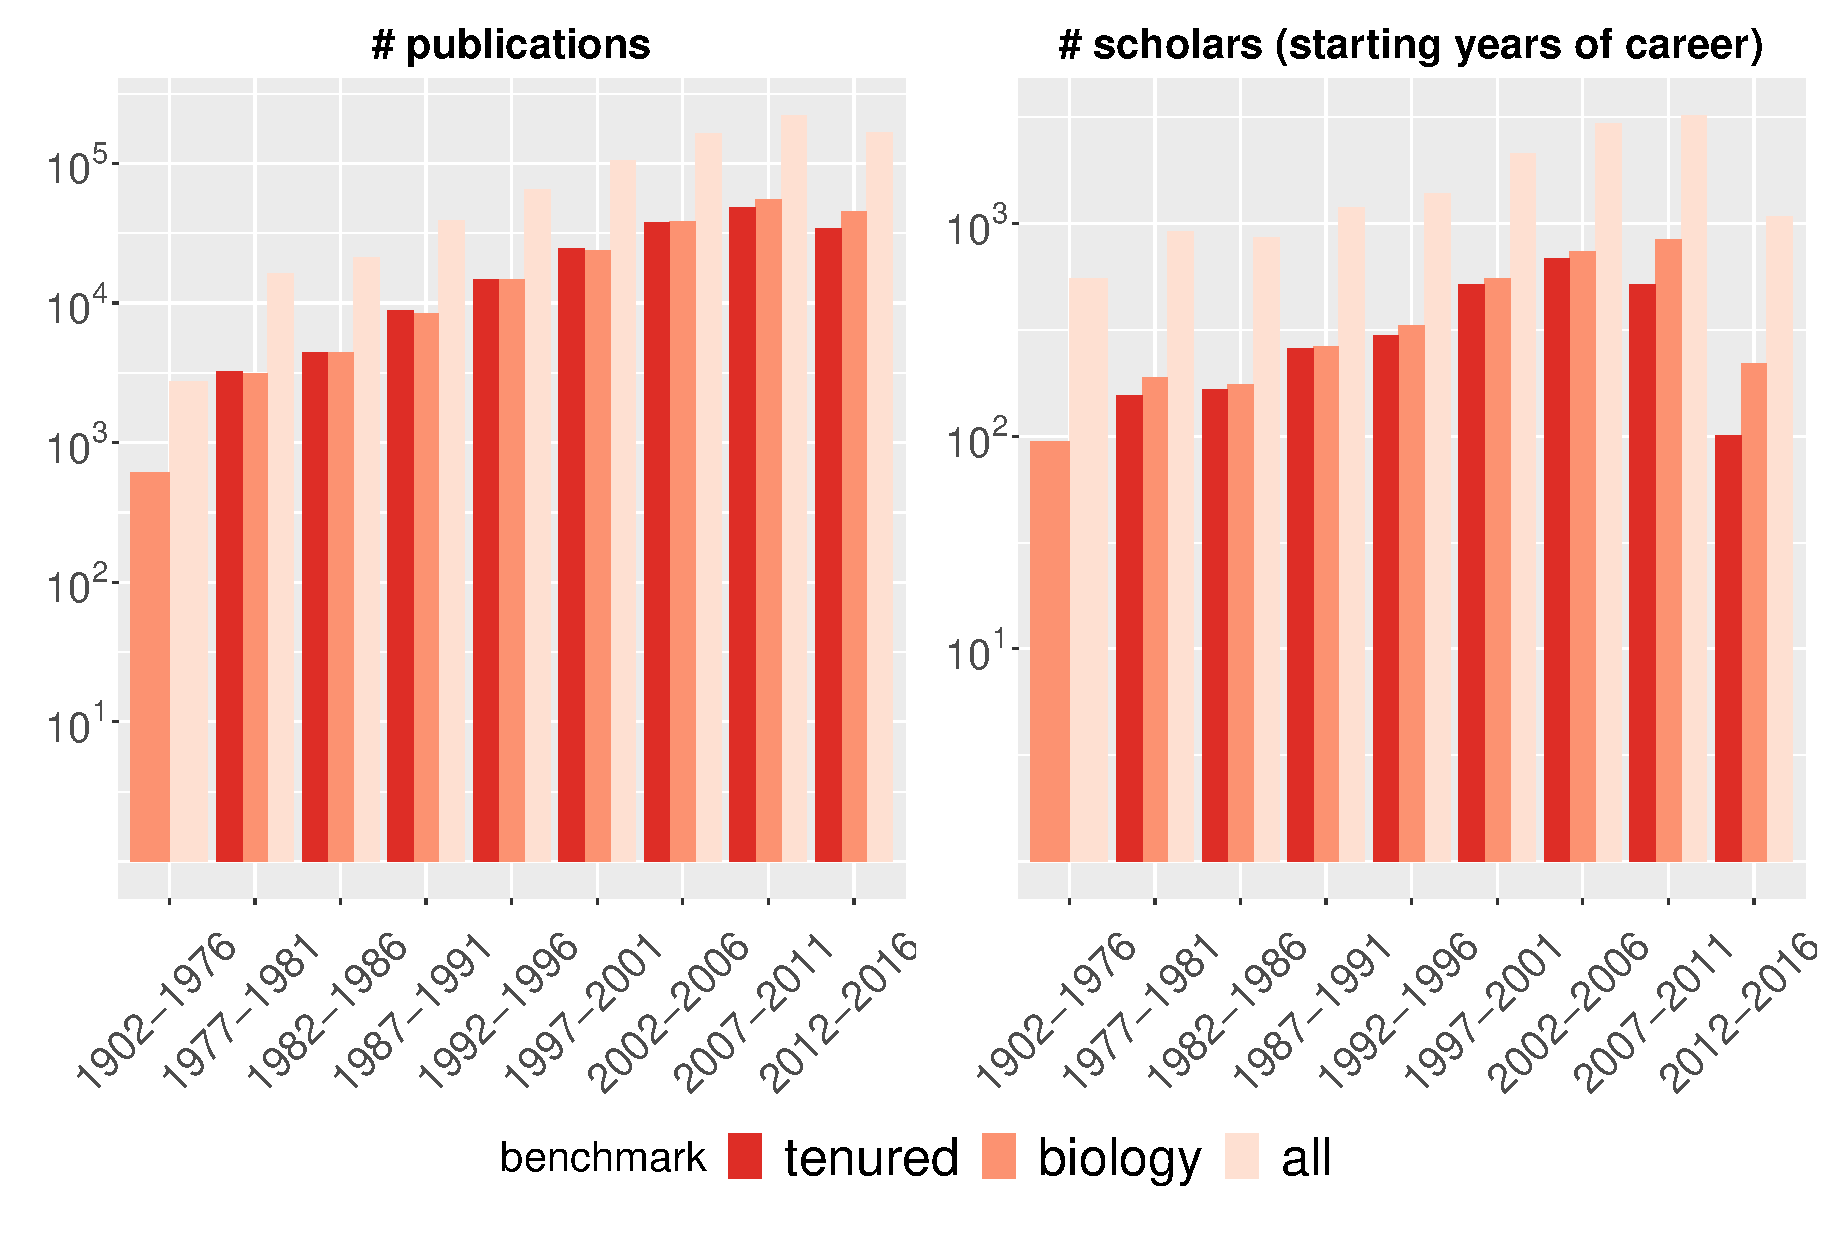
\includegraphics[width=0.8\textwidth]{figures/exploratory/npub_naut.eps}
    \caption[Exploratory statistics of the dataset]{\textbf{Left panel}: number of papers published in a certain period; \textbf{right panel}: number of authors who start their careers in a certain period. }
    \label{fig:exploratory}
\end{figure}

\begin{figure}[ht!]
    \centering
    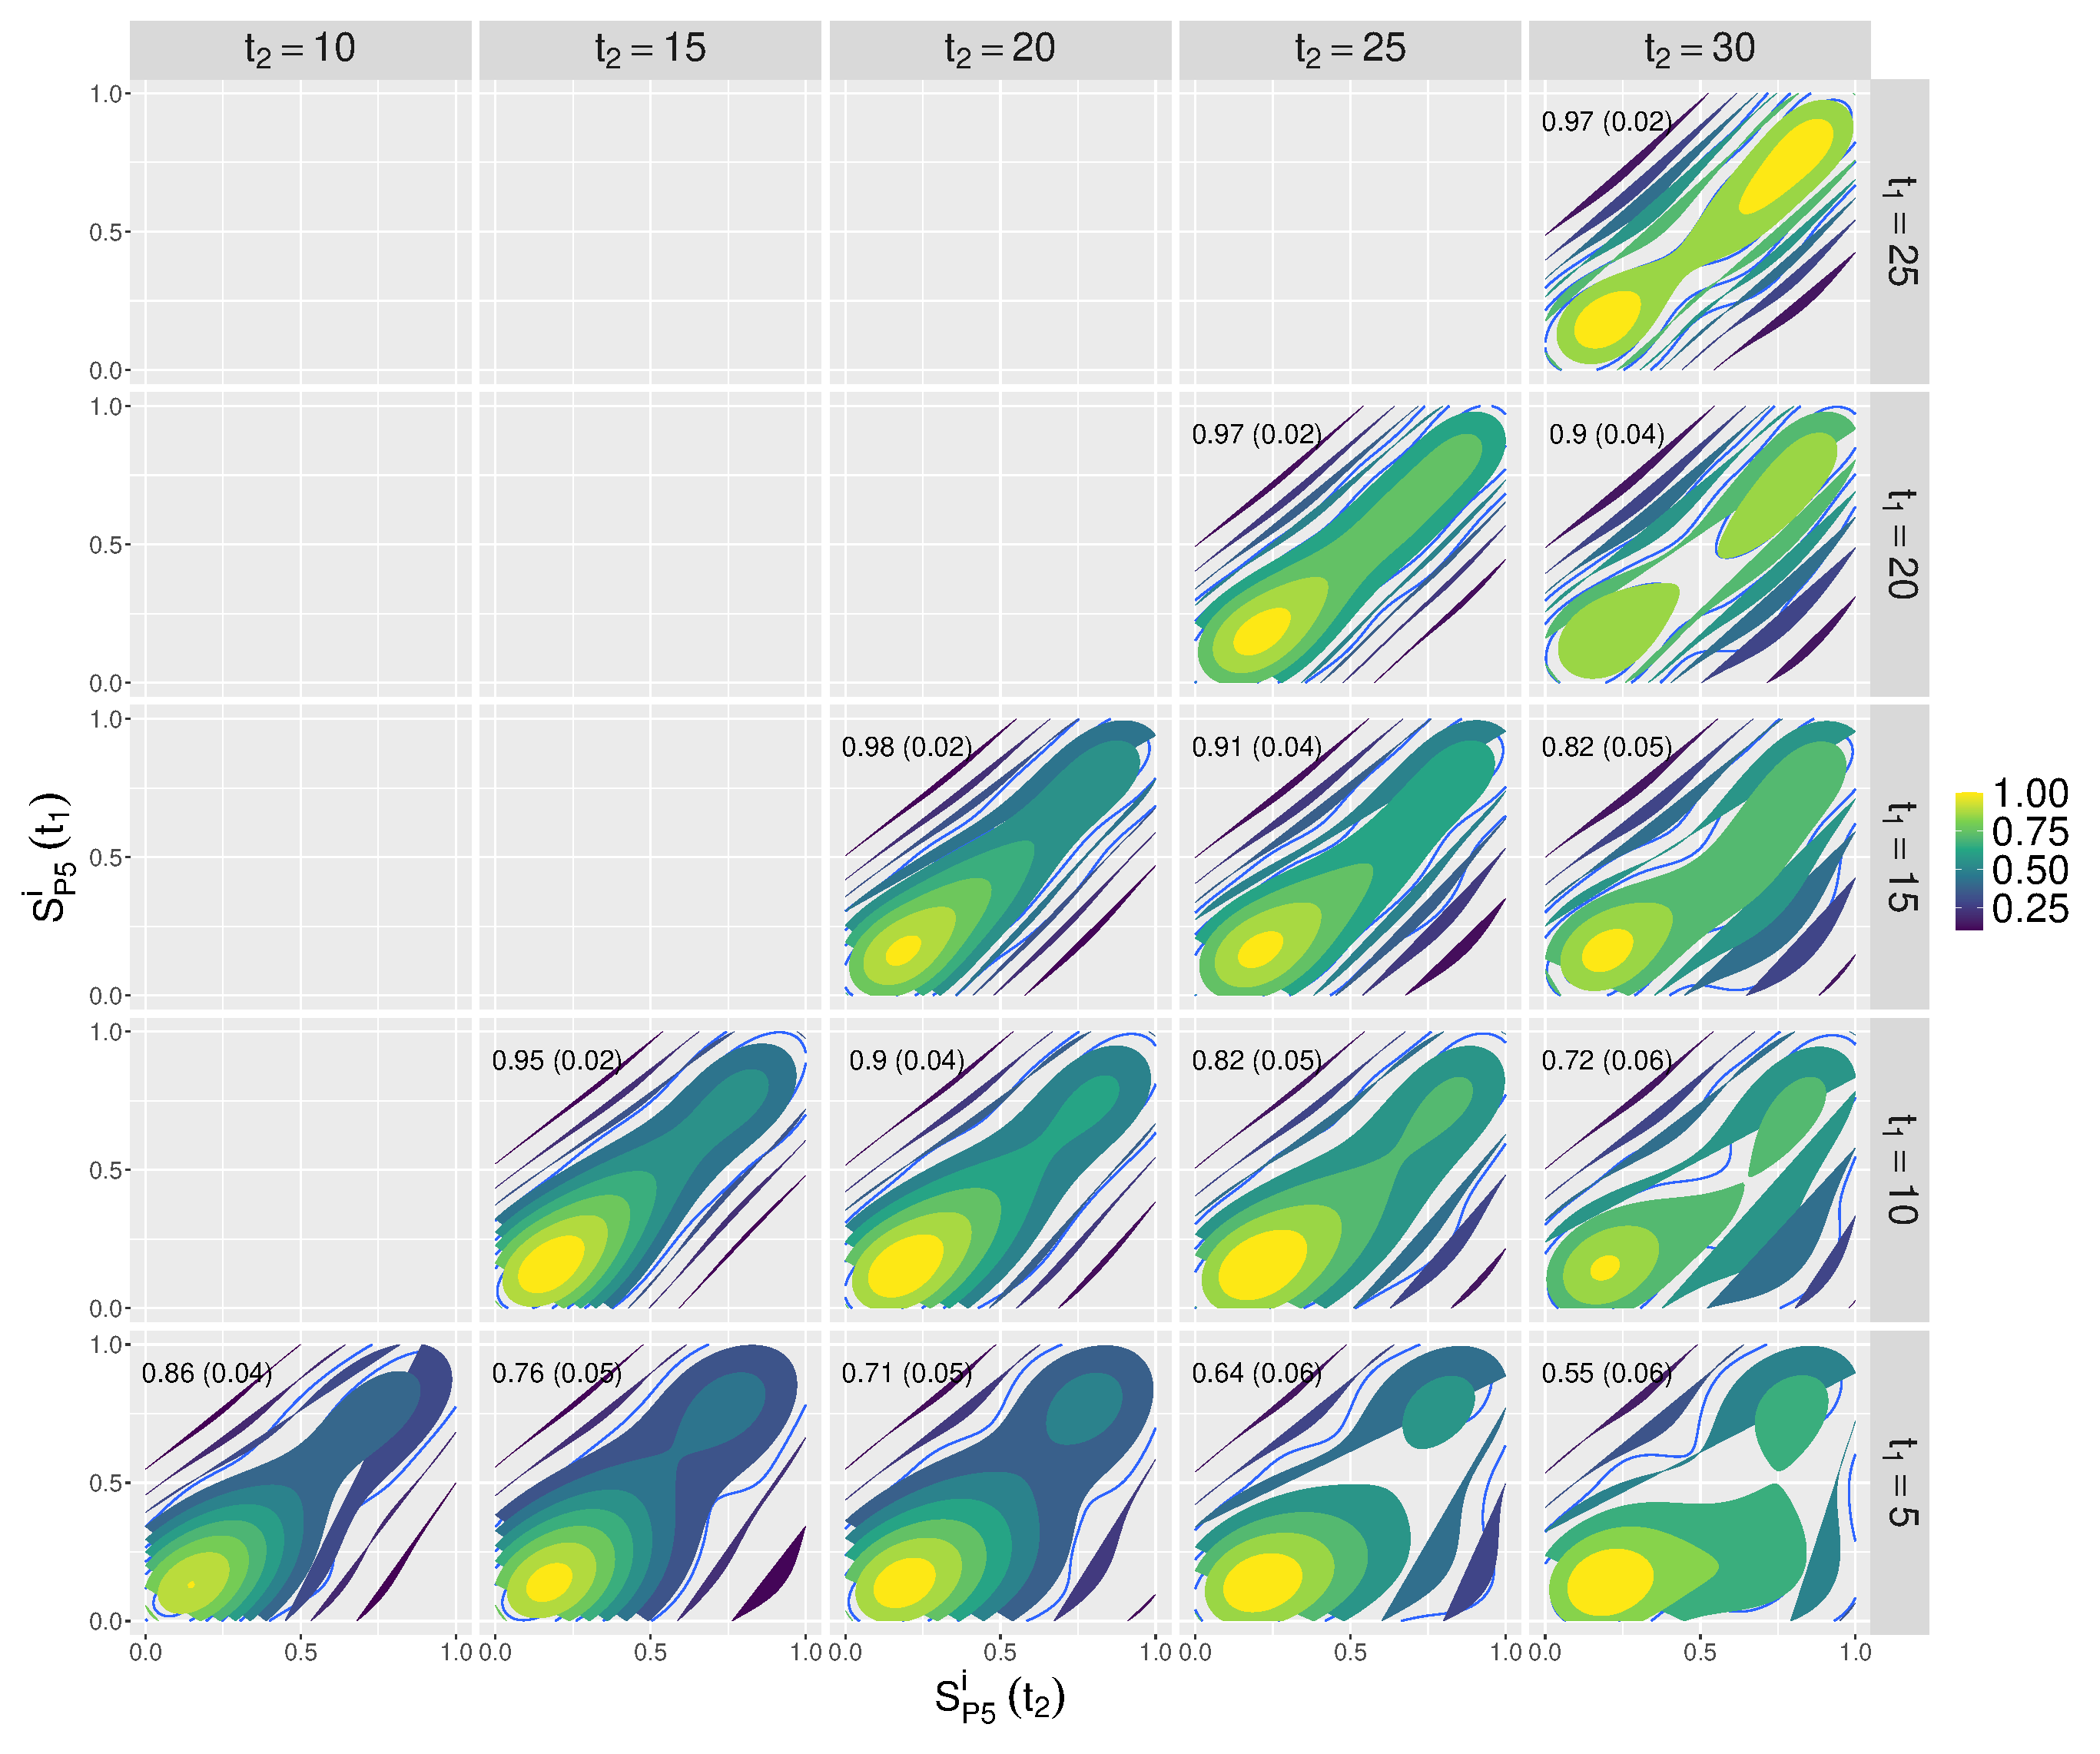
\includegraphics[width=\textwidth]{figures/pred_power/scatter_autrp_all.eps}
    \caption[Kernel density estimation for the scatters of S$_{P5}(t_1)$ and S$_{P5}(t_2)$]{Kernel density estimation for the scatter points of S$_{P5}^{ib}(t_1)$ and S$_{P5}^{ib}(t_2)$. We also fit a simple linear regression of S$_{P5}^{ib}(t_2)$ on S$_{P5}^{ib}(t_1)$. The estimated coefficient and the corresponding standard error (in the parentheses) are displayed in each plot.}
    \label{fig:scatter_autrp_all}
\end{figure}


\begin{figure}[ht!]
    \centering
    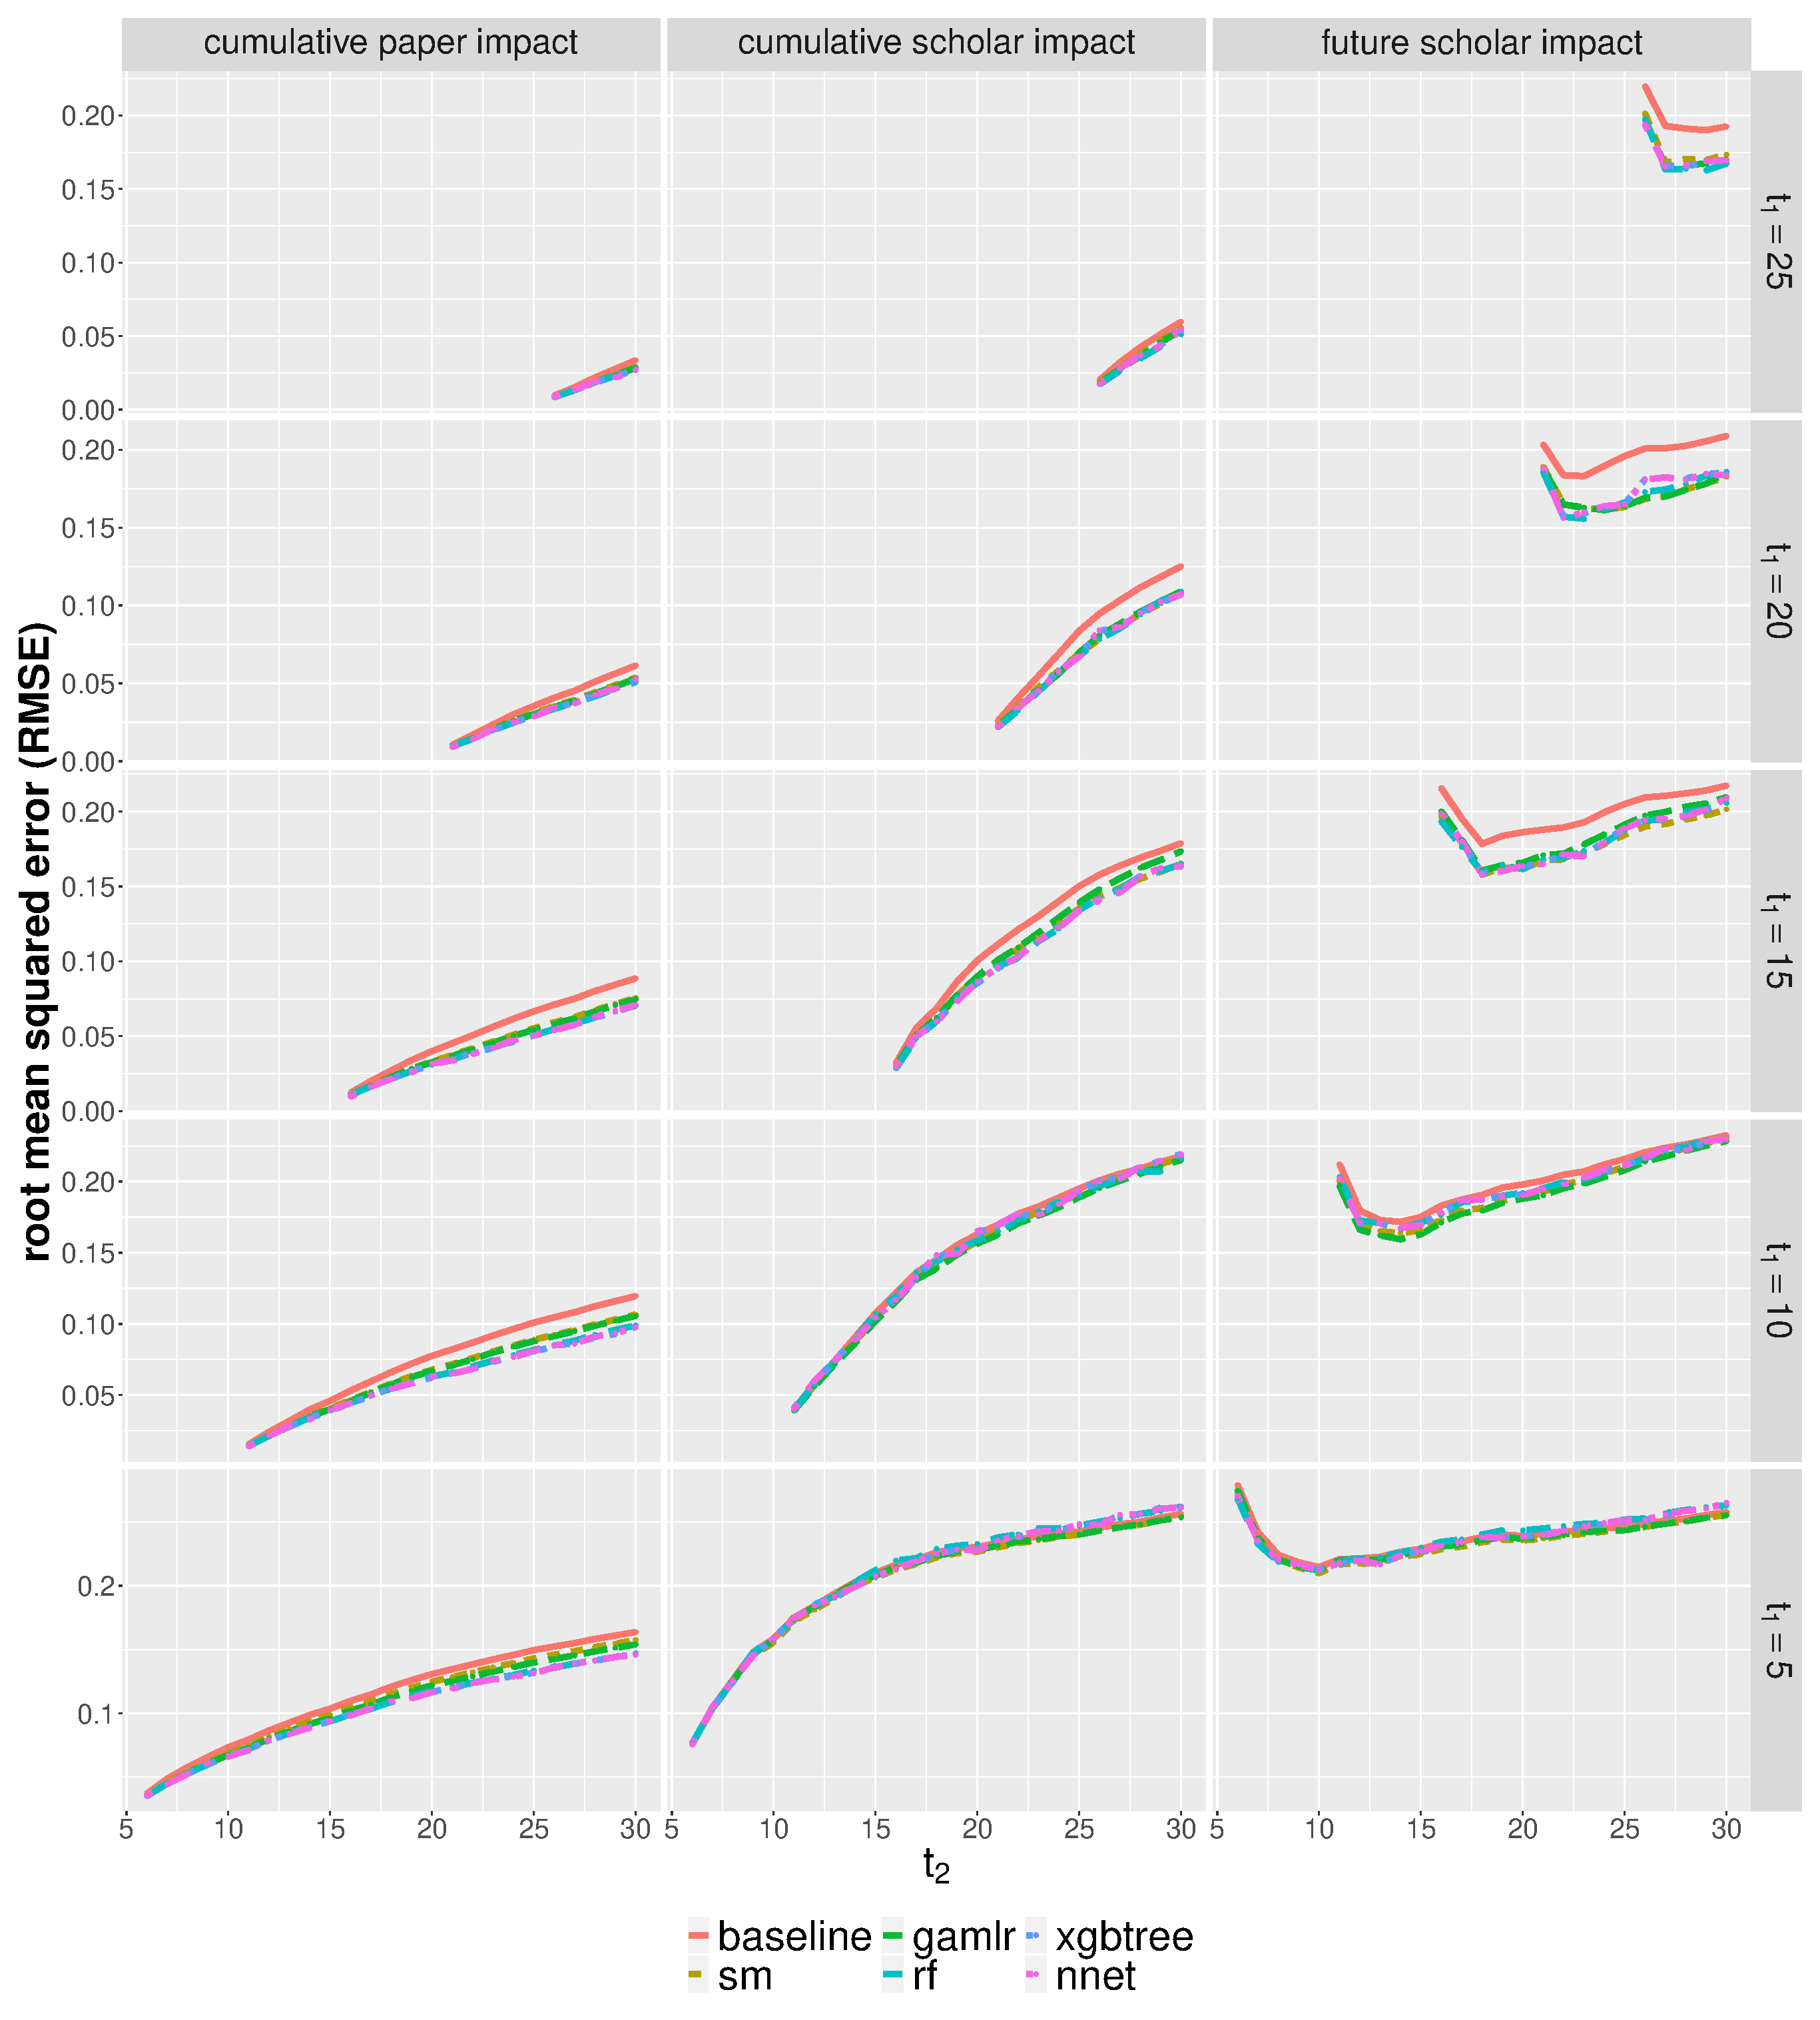
\includegraphics[width=\textwidth]{figures/pred_model/rmse.eps}
    \caption[RMSE of the predictive models]{Root mean squared error of the predictive models. The lasso, ridge and elastic net are outperformed by Gamma lasso, and hence are ignored for a better visualization.}
    \label{fig:pred_rmse}
\end{figure}

\begin{figure}[ht!]
    \centering
    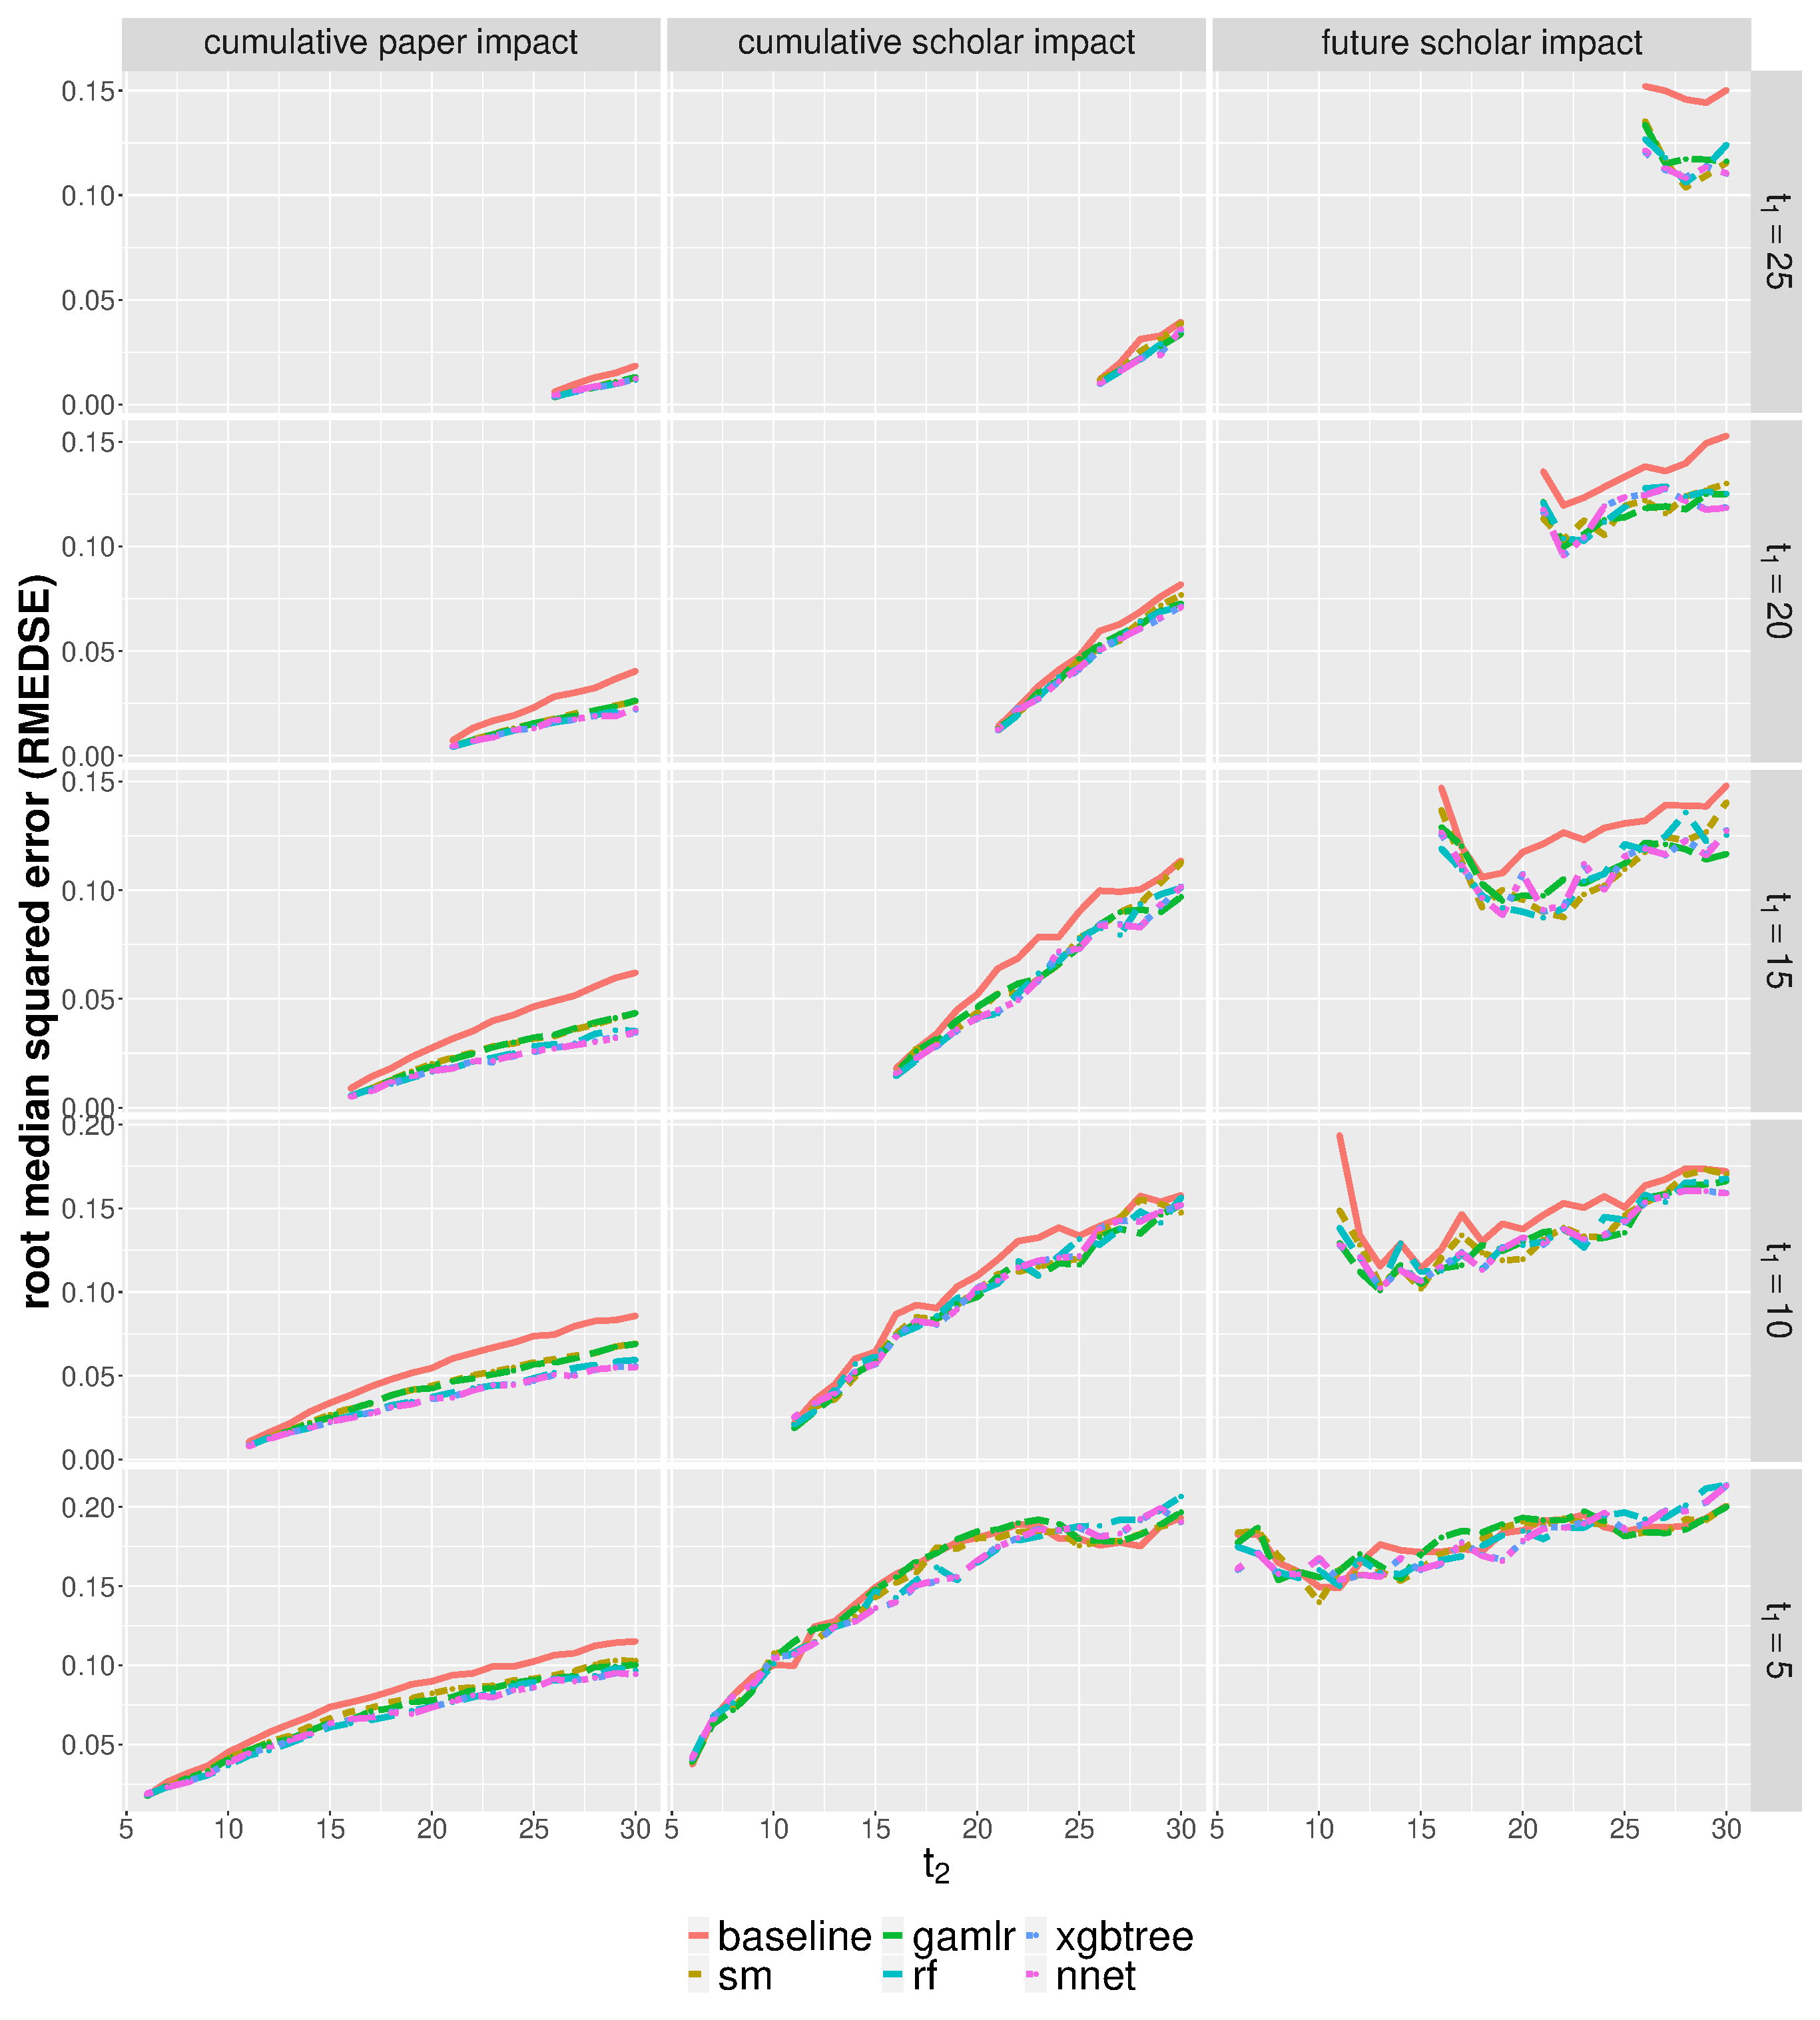
\includegraphics[width=\textwidth]{figures/pred_model/medse.eps}
    \caption[RMESE of the predictive models]{Root median squared error of the predictive models.}
    \label{fig:pred_medse}
\end{figure}

\begin{figure}[ht!]
    \centering
    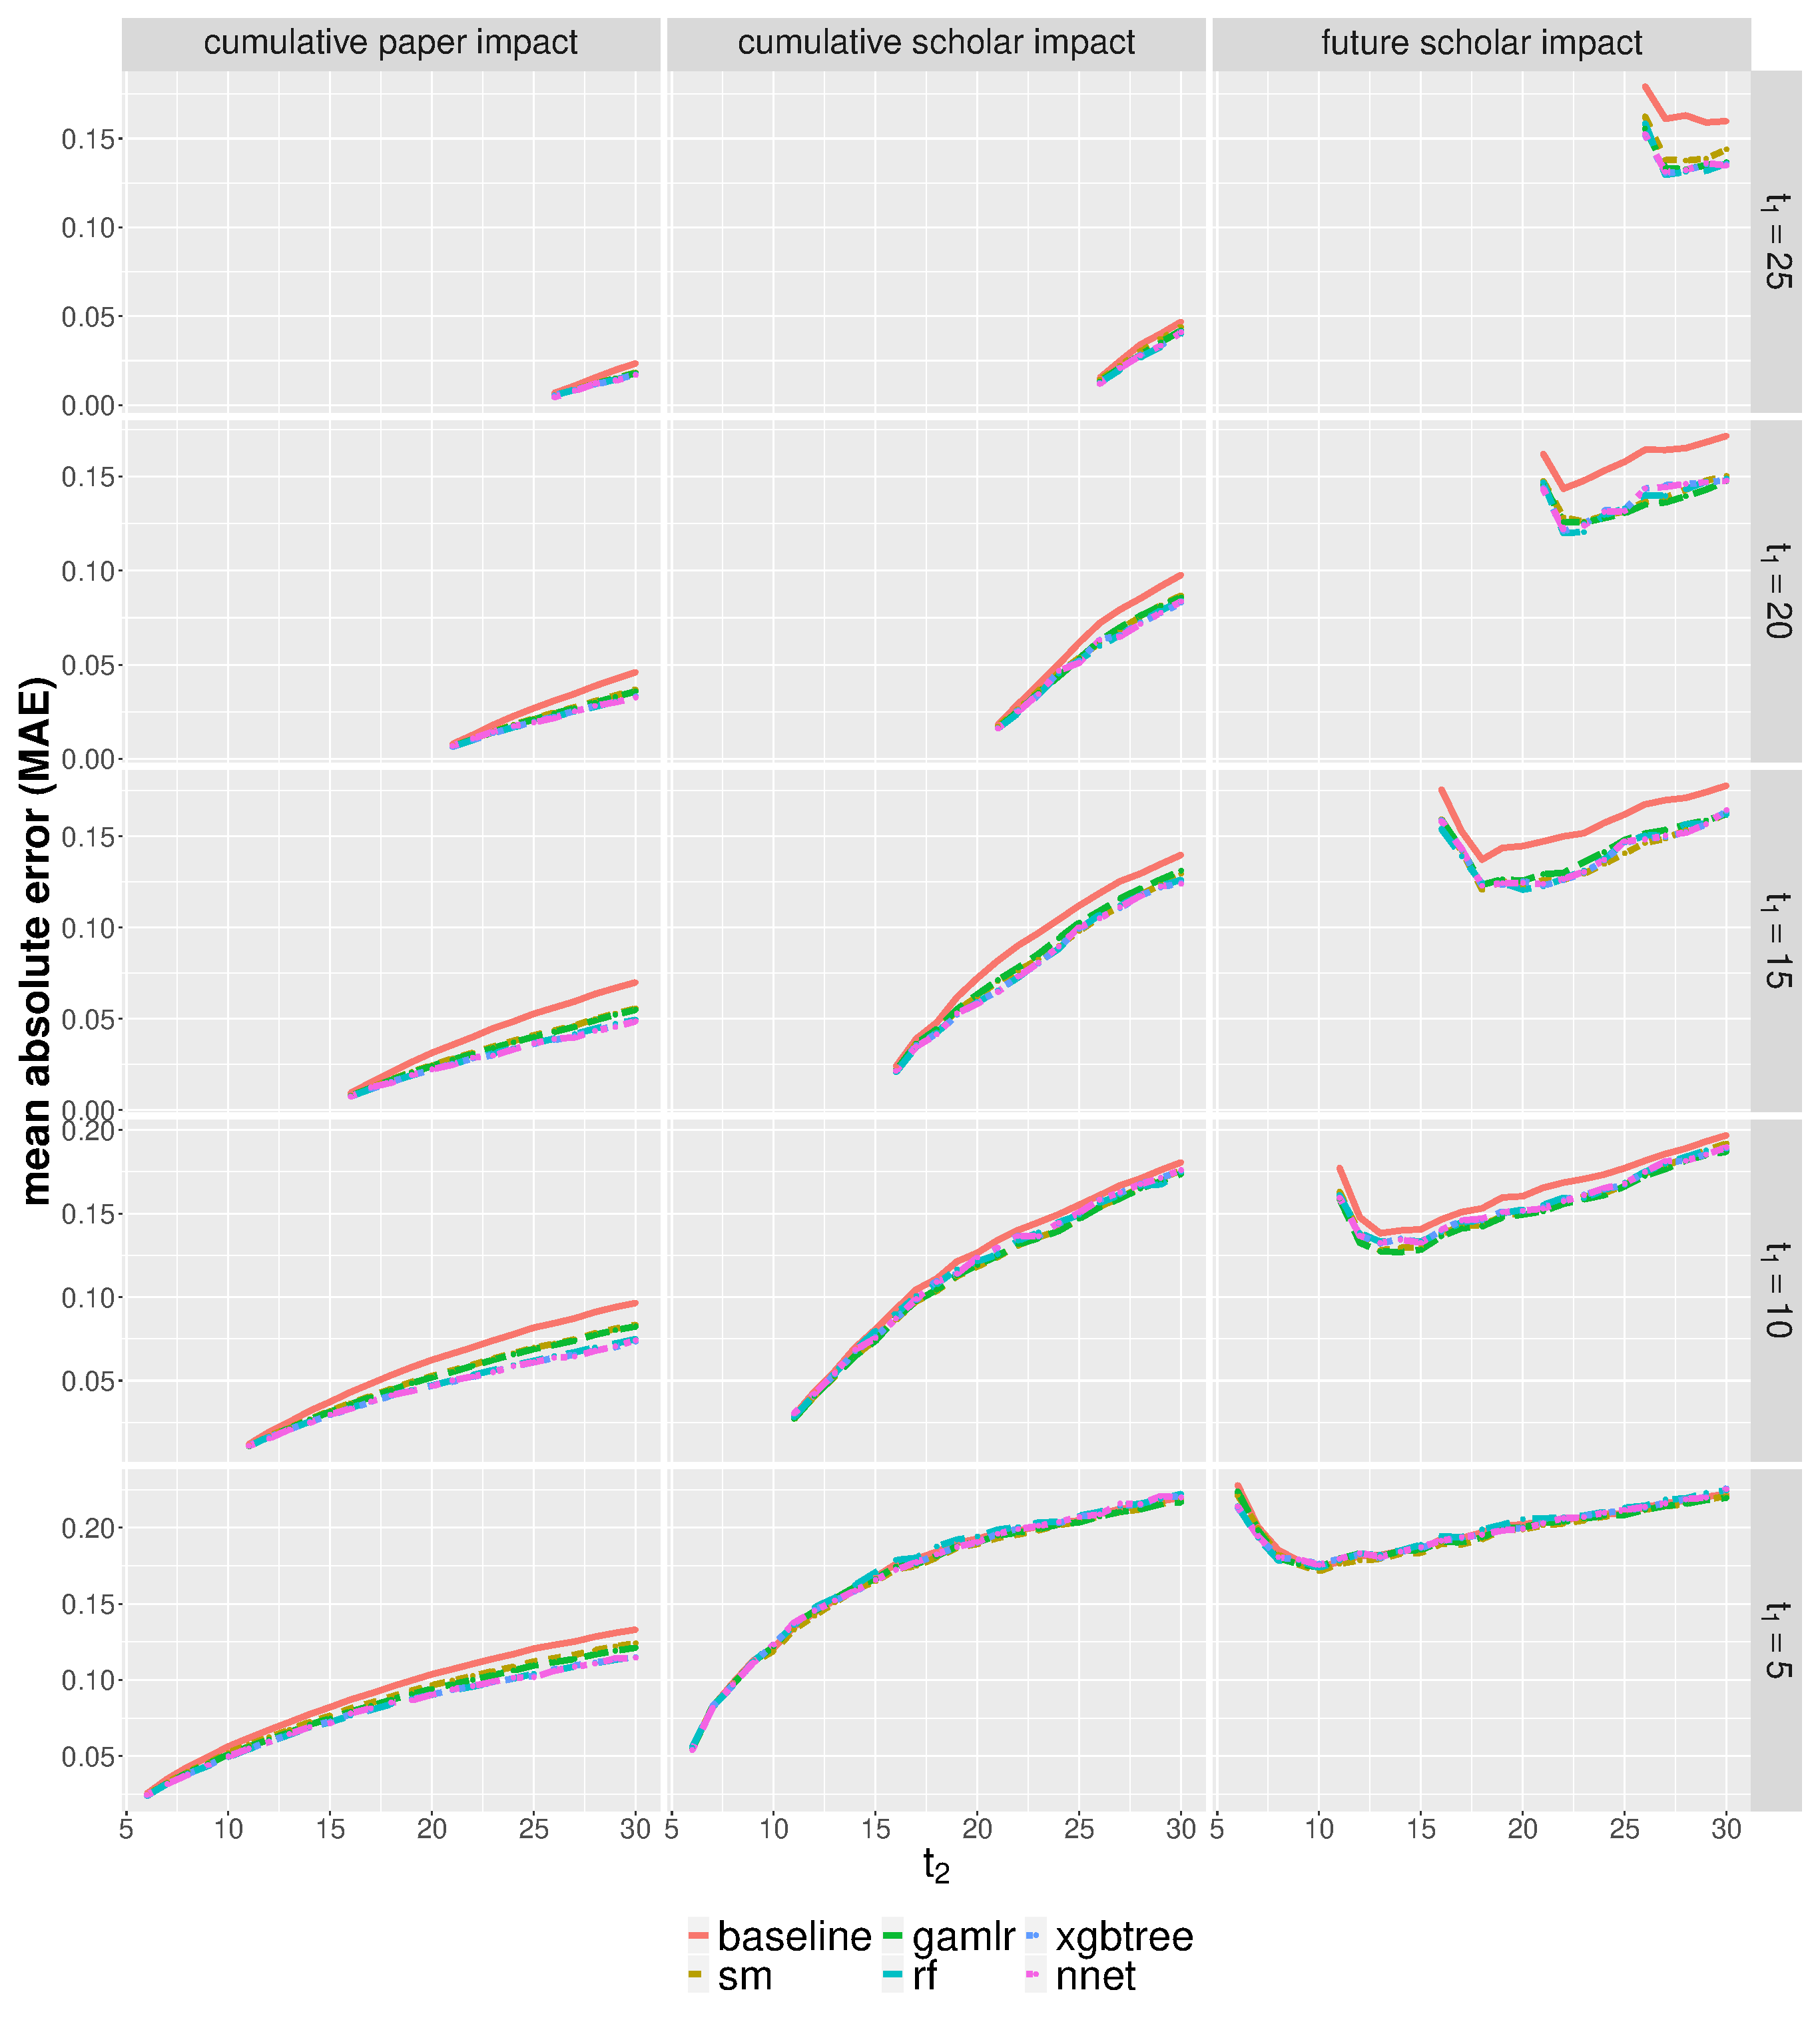
\includegraphics[width=\textwidth]{figures/pred_model/mae.eps}
    \caption[MAE of the predictive models]{Mean absolute error of the predictive models.}
    \label{fig:pred_mae}
\end{figure}

\iffalse
\clearpage
Three effects may lead to the non-stationarity of rank percentile for scholars are:
\begin{itemize}
  \item Seniority effect of scholars: senior scholars can attract more citations than junior scholars. In figure \ref{fig:seniority}, we see that senior authors (e.g. those starting their careers in 1980s) do not have an advantage over junior authors (e.g. those starting their careers in 2000s). 
  \item Time effect: papers published more recently attract more citations than papers published $20$ years ago. This maybe due to the fact that the entire scientific community is growing, and we have much more scholars now than $20$ years ago, which makes the paper visible to a larger audience and potentially attracts more citations. Meanwhile, as Internet and especially social media becomes vital, papers now have much better visibility than those $20$ years ago. Figure \ref{fig:environment} shows that for the scholars starting their careers in $1980$, more recent papers attract more citations than old papers. Since we've already filtered out the seniority effect of the scholars, this is result from external effects. 
  \item Number of publications: scholars now tend to produce more publications than scholars say $20$ years ago. Evidence is shown in figure \ref{fig:npub}. 
\end{itemize}
We now fix the bias from the time effect and number of publications, in order to get stationary rank percentile indicators for scholars. Let's say we have a scholar $i$ who starts his/her career in physical year $Y_i$. For a paper $j$ that the scholar publishes in physical year $Y_j$, we calculate its rank percentile rp.c$_{j5}$ where the benchmark contains all the papers that are published in year $Y_j$. By restricting the benchmark in such way, we potentially remove the time effect. We repeat the process for all the papers of scholar $i$ that are published by age $t$ and obtain the metric $\sum_{j=1}^{N_t^{(i)}} \text{rp.c}_{j5}$. Furthermore, we calculate a rank percentile indicator rp.p$_{it}$ based on the number of publications by age $t$, and the benchmark is all the scholars who start their careers in physical year $Y_i$. Finally, we have the evaluation metric m$_{it} = \text{rp.p}_{it} \cdot \sum_{j=1}^{N_t^{(i)}} \text{rp.c}_{j5}$. The rank percentile indicator, denoted as rp.rp5, can be then computed based on m$_{it}$ and the benchmark is all or biology. 

Figure \ref{fig:compare_autrp} shows various types of scholar rank percentile indicators. Both rp.c and rp.h, that are based on total citations and h-index, show advantages for junior scholars due to the reasons explained above. However, rp.rp5 seems to be stationary. 


\begin{figure}[h!]
     \centering
     \begin{subfigure}[b]{0.48\textwidth}
         \centering
         \includegraphics[width=\textwidth]{figures/exploratory/seniority_age5.eps}
         \caption{Total citations by age $5$ for papers published in $2012$}
     \end{subfigure}
     \hfill
     \begin{subfigure}[b]{0.5\textwidth}
         \centering
         \includegraphics[width=\textwidth]{figures/exploratory/seniority_age10.eps}
         \caption{Total citations by age $10$ for papers published in $2007$}
     \end{subfigure}
    \caption{Seniority effect of scholars. The x-axis indicates starting years of careers of the corresponding authors. There's no evidence that senior scholars can attract more citations than junior scholars.}
    \label{fig:seniority}
\end{figure}

\begin{figure}[h!]
     \centering
     \begin{subfigure}[b]{0.48\textwidth}
         \centering
         \includegraphics[width=\textwidth]{figures/exploratory/environment_age5.eps}
         \caption{Total citations by age $5$}
     \end{subfigure}
     \hfill
     \begin{subfigure}[b]{0.48\textwidth}
         \centering
         \includegraphics[width=\textwidth]{figures/exploratory/environment_age10.eps}
         \caption{Total citations by age $10$}
     \end{subfigure}
    \caption{Time effect. We consider the citations of the papers published by scholars who start their careers in year $1980$. The x-axis indicates the years of publication for their papers. We observe that more recent papers attract more citations than old papers.}
    \label{fig:environment}
\end{figure}

\begin{figure}[h!]
     \centering
     \begin{subfigure}[b]{0.48\textwidth}
         \centering
         \includegraphics[width=\textwidth]{figures/exploratory/npub_age5.eps}
         \caption{Number of publications by age $5$}
     \end{subfigure}
     \hfill
     \begin{subfigure}[b]{0.48\textwidth}
         \centering
         \includegraphics[width=\textwidth]{figures/exploratory/npub_age10.eps}
         \caption{Number of publications by age $10$}
     \end{subfigure}
    \caption{Number of publications. The x-axis indicates the starting years of careers of scholars. }
    \label{fig:npub}
\end{figure}


\begin{figure}[h!]
     \centering
     \begin{subfigure}[b]{0.48\textwidth}
         \centering
         \includegraphics[width=\textwidth]{figures/exploratory/rpc_age5.eps}
         \caption{rp.c$_{i5}$}
     \end{subfigure}
     \hfill
     \begin{subfigure}[b]{0.48\textwidth}
         \centering
         \includegraphics[width=\textwidth]{figures/exploratory/rpc_age10.eps}
         \caption{rp.c$_{i10}$}
     \end{subfigure}
     \hfill
      \begin{subfigure}[b]{0.48\textwidth}
         \centering
         \includegraphics[width=\textwidth]{figures/exploratory/rph_age5.eps}
         \caption{rp.h$_{i5}$}
     \end{subfigure}
     \hfill
     \begin{subfigure}[b]{0.48\textwidth}
         \centering
         \includegraphics[width=\textwidth]{figures/exploratory/rph_age10.eps}
         \caption{rp.h$_{i10}$}
     \end{subfigure}
      \hfill
      \begin{subfigure}[b]{0.48\textwidth}
         \centering
         \includegraphics[width=\textwidth]{figures/exploratory/rprp5new_age5.eps}
         \caption{rp.rp5$_{i5}$}
     \end{subfigure}
     \hfill
     \begin{subfigure}[b]{0.48\textwidth}
         \centering
         \includegraphics[width=\textwidth]{figures/exploratory/rprp5new_age10.eps}
         \caption{rp.rp5$_{i10}$}
     \end{subfigure}
    \caption{Different types of rank percentile indicators for scholars. rp.rp5 is stationary, while the other two are not.}
    \label{fig:compare_autrp}
\end{figure}

\fi

\end{refsection}



\end{document}
